\documentclass[12pt, a4]{book}
\usepackage[utf8]{inputenc}
\usepackage{amsmath,amsthm,amsfonts,amssymb,amscd}
\usepackage[table]{xcolor}
\usepackage[margin=2.5cm]{geometry}
\usepackage{ragged2e}
\usepackage{graphicx}
\usepackage{multicol}
\usepackage[brazil]{babel}
\usepackage{float}
\usepackage{hyperref}
\usepackage{lettrine}
\usepackage{emptypage}
\usepackage[sfdefault]{FiraSans} 
\usepackage{FiraMono}
\usepackage[T1]{fontenc}
\renewcommand*\oldstylenums[1]{{\firaoldstyle #1}}
\usepackage[cm]{sfmath}  

\begin{document}
	
	% Análise Municipal
	\chapter{Análise Municipal}
\label{cap:sp}

\lettrine{A}{} análise do atendimento das creches da cidade de São Paulo foi baseada na junção dos dados de todos os distritos. A seguir, é mostrado um panorama das matrículas e da demanda ao longo dos 12 anos analisado.

A \autoref{fig:saopaulo} mostra um gráfico com a evolução do atendimento no município.

\begin{figure}[H]
	\centering
	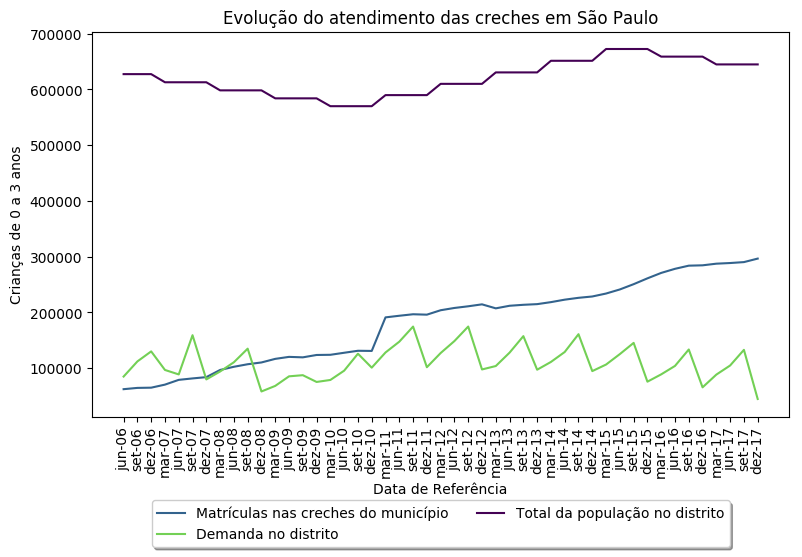
\includegraphics[width=0.7\linewidth]{../Analises/graficos/sao_paulo}
	\caption{Evolução das matrículas, da demanda, e da população de 0 a 3 anos no município de São Paulo.}
	\label{fig:saopaulo}
\end{figure}

É possível notar que existe uma sazonalidade na fila. Ela aumenta durante o ano e cai em dezembro. Nesse mês, parte dos alunos deixa as creches. Com isso, crianças deixam a fila e tornam-se matriculados.

Observa-se também que as matrículas possuem um crescimento constante, menos ao redor de 2010, quando a rede conveniada passou a ser contada e isso causou um aumento notável. 

Além disso, somando as matrículas com a demanda, percebe-se esse número não chega a 100\% da população de 0 a 3 anos. Isso ocorre porque parte dessa população fica na própria casa com os pais ou com outros familiares, já que a matrícula em creches não é obrigatória. Outras crianças são matriculadas na rede privada de ensino.

Para evidenciar que o atendimento melhorou no município como um todo, podem ser analisados o primeiro dado, de junho de 2006 e o último dado, de dezembro de 2017, na \autoref{tab:saopaulo}.

Pode-se observar que o número absoluto de matrículas no fim de 2017 é em torno de 5 vezes maior do que era no meio de 2006. O atendimento chegou a 45.93\% da população nessa faixa etária. Além disso, nota-se no gráfico que o número de matrículas tende a crescer.

\begin{table}[H]
	\begin{tabular}{l|l|l|l}
		\textbf{}                                 & \textbf{junho de 2006} & \textbf{dezembro de 2017} & \textbf{Variação} \\ \hline
		\textbf{Número de matrículas}             & 61729                  & 296260                    & +379.94\%       \\ \hline
		\textbf{Crianças na fila}                 & 84408                  & 44092                     & -47.76\%        \\ \hline
		\textbf{População de 0 a 3 anos estimada} & 627552                 & 644996                    & +2.78\%         \\ \hline
		\textbf{Matrículas relativas à população} & 9.84\%              & 45.93\%               & +366.77\%       \\ \hline
		\textbf{Fila relativa à população}        & 13.45\%             & 6.84\%                 & -49.14\%        \\
	\end{tabular}
	\caption{Comparação do primeiro período com o último analisado.}
	\label{tab:saopaulo}
\end{table}

O dado referente à fila induz a um erro de interpretação. Embora o objetivo dessa parte da análise seja comparar a primeira coleta de dados com a última, é injusto comparar a demanda em diferentes épocas do ano, por causa da sazonalidade associada a ela.

O ideal é comparar a demanda amostrada no mesmo mês do ano. A \autoref{tab:demanda} exibe a informação que permite uma análise melhor.

\begin{table}[H]
	\begin{tabular}{l|l|l|l}
		\textbf{}                                 & \textbf{dezembro de 2006} & \textbf{dezembro de 2017} & \textbf{Variação} \\ \hline
		\textbf{Crianças na fila}                 & 129594                    & 44092                     & -65.98\%       \\ \hline
		\textbf{População de 0 a 3 anos estimada} & 627552                    & 644996                    & +2.78\%        \\ \hline
		\textbf{Fila relativa à população}        & 20.65\%               & 6.84\%                  & -66.88\%        \\ 
	\end{tabular}
	\caption{Comparação da demanda no mês de dezembro, em 2006 e 2017.}
	\label{tab:demanda}
\end{table}

Algo ainda a ser observado em relação à fila é que há uma tendência de queda. A sazonalidade atrapalha nessa visualização, mas é possível ver que os vales são cada vez menores. Tal tendência é confirmada pelas análises preditivas, exibidas pelo \autoref{cap:tendencias}.
	
	% Análises Distritais
	\chapter{Análise Distrital}
\label{cap:dist}

\lettrine{P}{ara} cada um dos 96 distritos da cidade, foi feita uma análise como a municipal. Essas análises são um pouco menos verborrágicas, já que os distritos são muitos. Tal decisão foi tomada levando em conta que a maioria esmagadora dos distritos tem um comportamento muito semelhante ao município. As análises podem ser encontradas no \autoref{cap:apendDist}.

Em todos os distritos, foi observada uma sazonalidade na fila. Mesmo tendo seus picos, a demanda segue uma trajetória descendente. Comparando apenas os meses de dezembro, por causa desse efeito de temporada, quase todos os distritos diminuíram a fila, entre 2006 e 2017. Os únicos que tiveram um aumento na fila foram Marsilac, Pedreira e Vila Andrade.

As matrículas apresentaram um crescimento mais linear, sem grandes surpresas na trajetória. Olhando o primeiro dado, de junho de 2006, e o último dado, de dezembro de 2017, apenas a República teve uma redução no número de alunos matriculados. Todos os outros apresentaram aumento.

Ter uma demanda maior do que a capacidade de matrículas pode ser considerado um problema. Em 63 distritos, em junho de 2006, havia mais crianças na fila do que matriculadas em creches. Já em dezembro de 2017, apenas um distrito, a Sé, possuía essa condição, o menor número já registrado. A evolução do número de distritos nessa conjuntura pode ser vista na \autoref{graf:dem}.

\begin{figure}
	\centering
	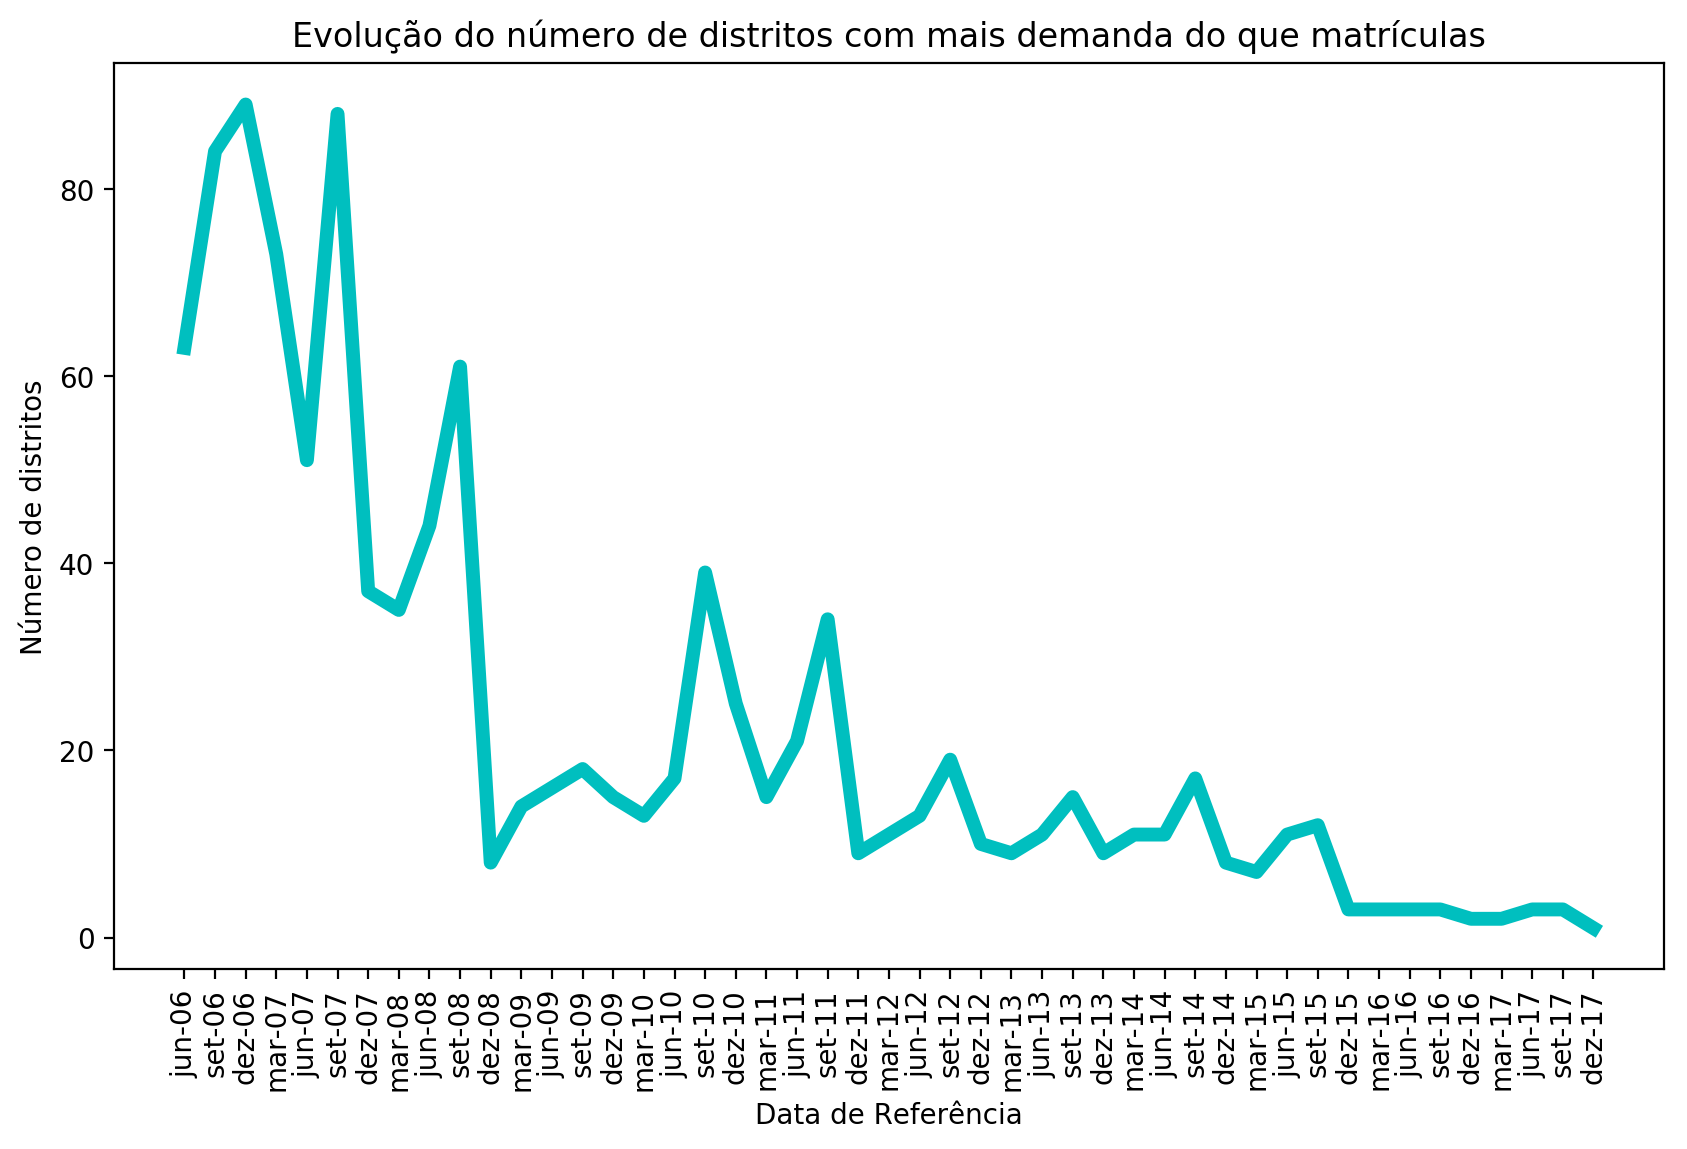
\includegraphics[width=.8\linewidth]{grafdem}
	\caption{Evolução do número de distritos com mais fila que matrículas.}
	\label{graf:dem}
\end{figure}

É curioso observar que esse número nunca chega a zero, nos períodos observados. O seu pico máximo foi atingido em dezembro de 2006, com 89 distritos nessa situação. 

Finalmente, destaque para alguns distritos. Para Marsilac, Jaguara e Lajeado, que atendem mais de 80\% da população estimada de 0 a 3 anos. Desses três, Lajeado tem o maior número de matrículas. No entanto, Marsilac pode ser considerado um \textit{outlier}, pois mesmo atendendo mais de 100\% da população considerada, ele tem a maior fila proporcional à população entre todos os distritos (26.6\%).


	
	% Rankings de 2006 e 2017
	\chapter{\textit{Rankings}}
	\label{cap:rankings}
	
	% Análises Preditivas
	\chapter{Análises Preditivas}
	\label{cap:preditivas}
	
	\appendix
	\chapter{Dados da Análise Distrital}
\label{cap:apendDist}

\lettrine{A}{s} análises apresentadas a seguir seguem um padrão, com os dados sendo apresentados de maneira muito parecida com a Análise Municipal. São divididas em três partes, sendo uma figura e duas tabelas.

A figura mostra duas informações: a primeira é um gráfico que mostra a evolução do atendimento e da população no distrito; a segunda é a localização do distrito no município.

A primeira tabela exibe as informações do primeiro período analisado e do último, junho de 2006 e dezembro de 2017, respectivamente. Assim como na análise do município, ela mostra o número de matrículas, o número de crianças na fila, a população de 0 a 3 anos estimada e as matrículas e fila relativas à população do distrito.

Além disso, essa tabela apresenta informações comparativas do distrito com o município. Cinco novas linhas foram adicionadas. As três primeiras exibem qual a proporção que as matrículas, a demanda e a população do distrito representam em relação aos dados municipais. As últimas duas mostram a localização do distrito em dois \textit{rankings}: um referente ao número de matrículas e o outro, ao tamanho da demanda. Tais listagens são exibidas na íntegra no \autoref{cap:rankings}.

Como essa informação pode levar a erros de interpretação, sobre a demanda, como escrito no \autoref{cap:sp}, foi colocado também uma tabela que faz uma comparação entre a demanda nos meses de dezembro de 2006 e dezembro de 2017, assim como na Análise Municipal.
	\section{Água Rasa}
\begin{figure}[H]
\centering
\includegraphics[width=0.66\linewidth]{../Analises/graficos/tempo/tempo_AGUA_RASA}
\includegraphics[width=0.33\linewidth]{../Analises/mapas/mapas/distrito_ARA}
\caption{Evolução das matrículas, da demanda, e da população de 0 a 3 anos no distrito Água Rasa e a sua localização no município, em azul-claro, respectivamente.}
\end{figure}
\begin{table}[H]
\begin{tabular}{l|l|l|l}
\textbf{}                                      & \textbf{junho de 2006}       & \textbf{dezembro de 2017}    & \textbf{Variação} \\ \hline
\textbf{Número de matrículas}                  & 573 & 1045 & 82.37\% \\ \hline
\textbf{Crianças na fila}                      & 505 & 102 & -79.8\% \\ \hline
\textbf{População de 0 a 3 anos estimada}      & 3468 & 3772 & 8.77\% \\ \hline
\textbf{Matrículas relativas à população}      & 16.52\% & 27.7\% & 67.68\% \\ \hline
\textbf{Fila relativa à população}             & 14.56\% & 2.7\% & -81.43\% \\ \hline
\textbf{Proporção das matrículas no município} & 0.93\% & 0.35\% & -62.0\% \\ \hline
\textbf{Proporção da demanda no município}     & 0.6\% & 0.23\% & -61.33\% \\ \hline
\textbf{Proporção da população de 0 a 3 anos}  & 0.55\% & 0.59\% & 5.97\% \\ \hline
\textbf{Posição no \textit{ranking} das matrículas}     & 41 & 69 & -28 \\ \hline
\textbf{Posição no \textit{ranking} da demanda}         & 56 & 81 & -25 \\ 
\end{tabular}
\caption{Comparação entre o primeiro e o último período da amostra}
\end{table}
\begin{table}[H]
\begin{tabular}{l|l|l|l}
\textbf{}                                 & \textbf{dezembro de 2006} & \textbf{dezembro de 2017} & \textbf{Variação} \\ \hline
\textbf{Crianças na fila}                      & 683 & 102 & -85.07\% \\ \hline
\textbf{População de 0 a 3 anos estimada}      & 3468 & 3772 & 8.77\% \\ \hline
\textbf{Fila relativa à população}             & 18.28\% & 2.7\% & -85.21\% \\
\end{tabular}
\caption{Comparação da demanda no mês de dezembro, em 2006 e 2017.}
\end{table}
\section{Alto de Pinheiros}
\begin{figure}[H]
\centering
\includegraphics[width=0.66\linewidth]{../Analises/graficos/tempo/tempo_ALTO_DE_PINHEIROS}
\includegraphics[width=0.33\linewidth]{../Analises/mapas/mapas/distrito_API}
\caption{Evolução das matrículas, da demanda, e da população de 0 a 3 anos no distrito Alto de Pinheiros e a sua localização no município, em azul-claro, respectivamente.}
\end{figure}
\begin{table}[H]
\begin{tabular}{l|l|l|l}
\textbf{}                                      & \textbf{junho de 2006}       & \textbf{dezembro de 2017}    & \textbf{Variação} \\ \hline
\textbf{Número de matrículas}                  & 236 & 404 & 71.19\% \\ \hline
\textbf{Crianças na fila}                      & 64 & 43 & -32.81\% \\ \hline
\textbf{População de 0 a 3 anos estimada}      & 1454 & 1340 & -7.84\% \\ \hline
\textbf{Matrículas relativas à população}      & 16.23\% & 30.15\% & 85.75\% \\ \hline
\textbf{Fila relativa à população}             & 4.4\% & 3.21\% & -27.1\% \\ \hline
\textbf{Proporção das matrículas no município} & 0.38\% & 0.14\% & -64.33\% \\ \hline
\textbf{Proporção da demanda no município}     & 0.08\% & 0.1\% & 28.62\% \\ \hline
\textbf{Proporção da população de 0 a 3 anos}  & 0.23\% & 0.21\% & -10.21\% \\ \hline
\textbf{Posição no \textit{ranking} das matrículas}     & 72 & 87 & -15 \\ \hline
\textbf{Posição no \textit{ranking} da demanda}         & 94 & 91 & 3 \\ 
\end{tabular}
\caption{Comparação entre o primeiro e o último período da amostra}
\end{table}
\begin{table}[H]
\begin{tabular}{l|l|l|l}
\textbf{}                                 & \textbf{dezembro de 2006} & \textbf{dezembro de 2017} & \textbf{Variação} \\ \hline
\textbf{Crianças na fila}                      & 170 & 43 & -74.71\% \\ \hline
\textbf{População de 0 a 3 anos estimada}      & 1454 & 1340 & -7.84\% \\ \hline
\textbf{Fila relativa à população}             & 17.06\% & 3.21\% & -81.19\% \\
\end{tabular}
\caption{Comparação da demanda no mês de dezembro, em 2006 e 2017.}
\end{table}
\section{Anhanguera}
\begin{figure}[H]
\centering
\includegraphics[width=0.66\linewidth]{../Analises/graficos/tempo/tempo_ANHANGUERA}
\includegraphics[width=0.33\linewidth]{../Analises/mapas/mapas/distrito_ANH}
\caption{Evolução das matrículas, da demanda, e da população de 0 a 3 anos no distrito Anhanguera e a sua localização no município, em azul-claro, respectivamente.}
\end{figure}
\begin{table}[H]
\begin{tabular}{l|l|l|l}
\textbf{}                                      & \textbf{junho de 2006}       & \textbf{dezembro de 2017}    & \textbf{Variação} \\ \hline
\textbf{Número de matrículas}                  & 207 & 2668 & 1188.89\% \\ \hline
\textbf{Crianças na fila}                      & 138 & 382 & 176.81\% \\ \hline
\textbf{População de 0 a 3 anos estimada}      & 4023 & 4660 & 15.83\% \\ \hline
\textbf{Matrículas relativas à população}      & 5.15\% & 57.25\% & 1012.7\% \\ \hline
\textbf{Fila relativa à população}             & 3.43\% & 8.2\% & 138.97\% \\ \hline
\textbf{Proporção das matrículas no município} & 0.34\% & 0.9\% & 168.55\% \\ \hline
\textbf{Proporção da demanda no município}     & 0.16\% & 0.87\% & 429.92\% \\ \hline
\textbf{Proporção da população de 0 a 3 anos}  & 0.64\% & 0.72\% & 12.86\% \\ \hline
\textbf{Posição no \textit{ranking} das matrículas}     & 79 & 41 & 38 \\ \hline
\textbf{Posição no \textit{ranking} da demanda}         & 89 & 29 & 60 \\ 
\end{tabular}
\caption{Comparação entre o primeiro e o último período da amostra}
\end{table}
\begin{table}[H]
\begin{tabular}{l|l|l|l}
\textbf{}                                 & \textbf{dezembro de 2006} & \textbf{dezembro de 2017} & \textbf{Variação} \\ \hline
\textbf{Crianças na fila}                      & 424 & 382 & -9.91\% \\ \hline
\textbf{População de 0 a 3 anos estimada}      & 4023 & 4660 & 15.83\% \\ \hline
\textbf{Fila relativa à população}             & 6.14\% & 8.2\% & 33.51\% \\
\end{tabular}
\caption{Comparação da demanda no mês de dezembro, em 2006 e 2017.}
\end{table}
\section{Aricanduva}
\begin{figure}[H]
\centering
\includegraphics[width=0.66\linewidth]{../Analises/graficos/tempo/tempo_ARICANDUVA}
\includegraphics[width=0.33\linewidth]{../Analises/mapas/mapas/distrito_ARI}
\caption{Evolução das matrículas, da demanda, e da população de 0 a 3 anos no distrito Aricanduva e a sua localização no município, em azul-claro, respectivamente.}
\end{figure}
\begin{table}[H]
\begin{tabular}{l|l|l|l}
\textbf{}                                      & \textbf{junho de 2006}       & \textbf{dezembro de 2017}    & \textbf{Variação} \\ \hline
\textbf{Número de matrículas}                  & 435 & 1583 & 263.91\% \\ \hline
\textbf{Crianças na fila}                      & 523 & 364 & -30.4\% \\ \hline
\textbf{População de 0 a 3 anos estimada}      & 4737 & 4156 & -12.27\% \\ \hline
\textbf{Matrículas relativas à população}      & 9.18\% & 38.09\% & 314.78\% \\ \hline
\textbf{Fila relativa à população}             & 11.04\% & 8.76\% & -20.67\% \\ \hline
\textbf{Proporção das matrículas no município} & 0.7\% & 0.53\% & -24.18\% \\ \hline
\textbf{Proporção da demanda no município}     & 0.62\% & 0.83\% & 33.24\% \\ \hline
\textbf{Proporção da população de 0 a 3 anos}  & 0.75\% & 0.65\% & -14.52\% \\ \hline
\textbf{Posição no \textit{ranking} das matrículas}     & 54 & 55 & -1 \\ \hline
\textbf{Posição no \textit{ranking} da demanda}         & 54 & 31 & 23 \\ 
\end{tabular}
\caption{Comparação entre o primeiro e o último período da amostra}
\end{table}
\begin{table}[H]
\begin{tabular}{l|l|l|l}
\textbf{}                                 & \textbf{dezembro de 2006} & \textbf{dezembro de 2017} & \textbf{Variação} \\ \hline
\textbf{Crianças na fila}                      & 717 & 364 & -49.23\% \\ \hline
\textbf{População de 0 a 3 anos estimada}      & 4737 & 4156 & -12.27\% \\ \hline
\textbf{Fila relativa à população}             & 9.71\% & 8.76\% & -9.8\% \\
\end{tabular}
\caption{Comparação da demanda no mês de dezembro, em 2006 e 2017.}
\end{table}
\section{Artur Alvim}
\begin{figure}[H]
\centering
\includegraphics[width=0.66\linewidth]{../Analises/graficos/tempo/tempo_ARTUR_ALVIM}
\includegraphics[width=0.33\linewidth]{../Analises/mapas/mapas/distrito_AAL}
\caption{Evolução das matrículas, da demanda, e da população de 0 a 3 anos no distrito Artur Alvim e a sua localização no município, em azul-claro, respectivamente.}
\end{figure}
\begin{table}[H]
\begin{tabular}{l|l|l|l}
\textbf{}                                      & \textbf{junho de 2006}       & \textbf{dezembro de 2017}    & \textbf{Variação} \\ \hline
\textbf{Número de matrículas}                  & 901 & 2620 & 190.79\% \\ \hline
\textbf{Crianças na fila}                      & 670 & 153 & -77.16\% \\ \hline
\textbf{População de 0 a 3 anos estimada}      & 5689 & 4910 & -13.69\% \\ \hline
\textbf{Matrículas relativas à população}      & 15.84\% & 53.36\% & 236.92\% \\ \hline
\textbf{Fila relativa à população}             & 11.78\% & 3.12\% & -73.54\% \\ \hline
\textbf{Proporção das matrículas no município} & 1.46\% & 0.88\% & -39.41\% \\ \hline
\textbf{Proporção da demanda no município}     & 0.79\% & 0.35\% & -56.28\% \\ \hline
\textbf{Proporção da população de 0 a 3 anos}  & 0.91\% & 0.76\% & -15.91\% \\ \hline
\textbf{Posição no \textit{ranking} das matrículas}     & 25 & 43 & -18 \\ \hline
\textbf{Posição no \textit{ranking} da demanda}         & 41 & 63 & -22 \\ 
\end{tabular}
\caption{Comparação entre o primeiro e o último período da amostra}
\end{table}
\begin{table}[H]
\begin{tabular}{l|l|l|l}
\textbf{}                                 & \textbf{dezembro de 2006} & \textbf{dezembro de 2017} & \textbf{Variação} \\ \hline
\textbf{Crianças na fila}                      & 1368 & 153 & -88.82\% \\ \hline
\textbf{População de 0 a 3 anos estimada}      & 5689 & 4910 & -13.69\% \\ \hline
\textbf{Fila relativa à população}             & 15.01\% & 3.12\% & -79.24\% \\
\end{tabular}
\caption{Comparação da demanda no mês de dezembro, em 2006 e 2017.}
\end{table}
\section{Barra Funda}
\begin{figure}[H]
\centering
\includegraphics[width=0.66\linewidth]{../Analises/graficos/tempo/tempo_BARRA_FUNDA}
\includegraphics[width=0.33\linewidth]{../Analises/mapas/mapas/distrito_BFU}
\caption{Evolução das matrículas, da demanda, e da população de 0 a 3 anos no distrito Barra Funda e a sua localização no município, em azul-claro, respectivamente.}
\end{figure}
\begin{table}[H]
\begin{tabular}{l|l|l|l}
\textbf{}                                      & \textbf{junho de 2006}       & \textbf{dezembro de 2017}    & \textbf{Variação} \\ \hline
\textbf{Número de matrículas}                  & 220 & 337 & 53.18\% \\ \hline
\textbf{Crianças na fila}                      & 196 & 26 & -86.73\% \\ \hline
\textbf{População de 0 a 3 anos estimada}      & 574 & 813 & 41.64\% \\ \hline
\textbf{Matrículas relativas à população}      & 38.33\% & 41.45\% & 8.15\% \\ \hline
\textbf{Fila relativa à população}             & 34.15\% & 3.2\% & -90.63\% \\ \hline
\textbf{Proporção das matrículas no município} & 0.36\% & 0.11\% & -68.08\% \\ \hline
\textbf{Proporção da demanda no município}     & 0.23\% & 0.06\% & -74.61\% \\ \hline
\textbf{Proporção da população de 0 a 3 anos}  & 0.09\% & 0.13\% & 38.0\% \\ \hline
\textbf{Posição no \textit{ranking} das matrículas}     & 75 & 92 & -17 \\ \hline
\textbf{Posição no \textit{ranking} da demanda}         & 82 & 93 & -11 \\ 
\end{tabular}
\caption{Comparação entre o primeiro e o último período da amostra}
\end{table}
\begin{table}[H]
\begin{tabular}{l|l|l|l}
\textbf{}                                 & \textbf{dezembro de 2006} & \textbf{dezembro de 2017} & \textbf{Variação} \\ \hline
\textbf{Crianças na fila}                      & 266 & 26 & -90.23\% \\ \hline
\textbf{População de 0 a 3 anos estimada}      & 574 & 813 & 41.64\% \\ \hline
\textbf{Fila relativa à população}             & 45.12\% & 3.2\% & -92.91\% \\
\end{tabular}
\caption{Comparação da demanda no mês de dezembro, em 2006 e 2017.}
\end{table}
\section{Bela Vista}
\begin{figure}[H]
\centering
\includegraphics[width=0.66\linewidth]{../Analises/graficos/tempo/tempo_BELA_VISTA}
\includegraphics[width=0.33\linewidth]{../Analises/mapas/mapas/distrito_BVI}
\caption{Evolução das matrículas, da demanda, e da população de 0 a 3 anos no distrito Bela Vista e a sua localização no município, em azul-claro, respectivamente.}
\end{figure}
\begin{table}[H]
\begin{tabular}{l|l|l|l}
\textbf{}                                      & \textbf{junho de 2006}       & \textbf{dezembro de 2017}    & \textbf{Variação} \\ \hline
\textbf{Número de matrículas}                  & 493 & 1509 & 206.09\% \\ \hline
\textbf{Crianças na fila}                      & 738 & 387 & -47.56\% \\ \hline
\textbf{População de 0 a 3 anos estimada}      & 2342 & 3350 & 43.04\% \\ \hline
\textbf{Matrículas relativas à população}      & 21.05\% & 45.04\% & 113.99\% \\ \hline
\textbf{Fila relativa à população}             & 31.51\% & 11.55\% & -63.34\% \\ \hline
\textbf{Proporção das matrículas no município} & 0.8\% & 0.51\% & -36.22\% \\ \hline
\textbf{Proporção da demanda no município}     & 0.87\% & 0.88\% & 0.39\% \\ \hline
\textbf{Proporção da população de 0 a 3 anos}  & 0.37\% & 0.52\% & 39.37\% \\ \hline
\textbf{Posição no \textit{ranking} das matrículas}     & 46 & 60 & -14 \\ \hline
\textbf{Posição no \textit{ranking} da demanda}         & 38 & 28 & 10 \\ 
\end{tabular}
\caption{Comparação entre o primeiro e o último período da amostra}
\end{table}
\begin{table}[H]
\begin{tabular}{l|l|l|l}
\textbf{}                                 & \textbf{dezembro de 2006} & \textbf{dezembro de 2017} & \textbf{Variação} \\ \hline
\textbf{Crianças na fila}                      & 808 & 387 & -52.1\% \\ \hline
\textbf{População de 0 a 3 anos estimada}      & 2342 & 3350 & 43.04\% \\ \hline
\textbf{Fila relativa à população}             & 25.83\% & 11.55\% & -55.28\% \\
\end{tabular}
\caption{Comparação da demanda no mês de dezembro, em 2006 e 2017.}
\end{table}
\section{Belém}
\begin{figure}[H]
\centering
\includegraphics[width=0.66\linewidth]{../Analises/graficos/tempo/tempo_BELEM}
\includegraphics[width=0.33\linewidth]{../Analises/mapas/mapas/distrito_BEL}
\caption{Evolução das matrículas, da demanda, e da população de 0 a 3 anos no distrito Belém e a sua localização no município, em azul-claro, respectivamente.}
\end{figure}
\begin{table}[H]
\begin{tabular}{l|l|l|l}
\textbf{}                                      & \textbf{junho de 2006}       & \textbf{dezembro de 2017}    & \textbf{Variação} \\ \hline
\textbf{Número de matrículas}                  & 154 & 1145 & 643.51\% \\ \hline
\textbf{Crianças na fila}                      & 285 & 198 & -30.53\% \\ \hline
\textbf{População de 0 a 3 anos estimada}      & 2058 & 3318 & 61.22\% \\ \hline
\textbf{Matrículas relativas à população}      & 7.48\% & 34.51\% & 361.16\% \\ \hline
\textbf{Fila relativa à população}             & 13.85\% & 5.97\% & -56.91\% \\ \hline
\textbf{Proporção das matrículas no município} & 0.25\% & 0.39\% & 54.92\% \\ \hline
\textbf{Proporção da demanda no município}     & 0.34\% & 0.45\% & 33.0\% \\ \hline
\textbf{Proporção da população de 0 a 3 anos}  & 0.33\% & 0.52\% & 57.08\% \\ \hline
\textbf{Posição no \textit{ranking} das matrículas}     & 84 & 67 & 17 \\ \hline
\textbf{Posição no \textit{ranking} da demanda}         & 75 & 51 & 24 \\ 
\end{tabular}
\caption{Comparação entre o primeiro e o último período da amostra}
\end{table}
\begin{table}[H]
\begin{tabular}{l|l|l|l}
\textbf{}                                 & \textbf{dezembro de 2006} & \textbf{dezembro de 2017} & \textbf{Variação} \\ \hline
\textbf{Crianças na fila}                      & 532 & 198 & -62.78\% \\ \hline
\textbf{População de 0 a 3 anos estimada}      & 2058 & 3318 & 61.22\% \\ \hline
\textbf{Fila relativa à população}             & 9.77\% & 5.97\% & -38.92\% \\
\end{tabular}
\caption{Comparação da demanda no mês de dezembro, em 2006 e 2017.}
\end{table}
\section{Bom Retiro}
\begin{figure}[H]
\centering
\includegraphics[width=0.66\linewidth]{../Analises/graficos/tempo/tempo_BOM_RETIRO}
\includegraphics[width=0.33\linewidth]{../Analises/mapas/mapas/distrito_BRE}
\caption{Evolução das matrículas, da demanda, e da população de 0 a 3 anos no distrito Bom Retiro e a sua localização no município, em azul-claro, respectivamente.}
\end{figure}
\begin{table}[H]
\begin{tabular}{l|l|l|l}
\textbf{}                                      & \textbf{junho de 2006}       & \textbf{dezembro de 2017}    & \textbf{Variação} \\ \hline
\textbf{Número de matrículas}                  & 452 & 910 & 101.33\% \\ \hline
\textbf{Crianças na fila}                      & 640 & 319 & -50.16\% \\ \hline
\textbf{População de 0 a 3 anos estimada}      & 1651 & 2392 & 44.88\% \\ \hline
\textbf{Matrículas relativas à população}      & 27.38\% & 38.04\% & 38.96\% \\ \hline
\textbf{Fila relativa à população}             & 38.76\% & 13.34\% & -65.6\% \\ \hline
\textbf{Proporção das matrículas no município} & 0.73\% & 0.31\% & -58.05\% \\ \hline
\textbf{Proporção da demanda no município}     & 0.76\% & 0.72\% & -4.58\% \\ \hline
\textbf{Proporção da população de 0 a 3 anos}  & 0.26\% & 0.37\% & 41.16\% \\ \hline
\textbf{Posição no \textit{ranking} das matrículas}     & 51 & 73 & -22 \\ \hline
\textbf{Posição no \textit{ranking} da demanda}         & 43 & 36 & 7 \\ 
\end{tabular}
\caption{Comparação entre o primeiro e o último período da amostra}
\end{table}
\begin{table}[H]
\begin{tabular}{l|l|l|l}
\textbf{}                                 & \textbf{dezembro de 2006} & \textbf{dezembro de 2017} & \textbf{Variação} \\ \hline
\textbf{Crianças na fila}                      & 711 & 319 & -55.13\% \\ \hline
\textbf{População de 0 a 3 anos estimada}      & 1651 & 2392 & 44.88\% \\ \hline
\textbf{Fila relativa à população}             & 28.59\% & 13.34\% & -53.35\% \\
\end{tabular}
\caption{Comparação da demanda no mês de dezembro, em 2006 e 2017.}
\end{table}
\section{Brás}
\begin{figure}[H]
\centering
\includegraphics[width=0.66\linewidth]{../Analises/graficos/tempo/tempo_BRAS}
\includegraphics[width=0.33\linewidth]{../Analises/mapas/mapas/distrito_BRS}
\caption{Evolução das matrículas, da demanda, e da população de 0 a 3 anos no distrito Brás e a sua localização no município, em azul-claro, respectivamente.}
\end{figure}
\begin{table}[H]
\begin{tabular}{l|l|l|l}
\textbf{}                                      & \textbf{junho de 2006}       & \textbf{dezembro de 2017}    & \textbf{Variação} \\ \hline
\textbf{Número de matrículas}                  & 199 & 511 & 156.78\% \\ \hline
\textbf{Crianças na fila}                      & 253 & 304 & 20.16\% \\ \hline
\textbf{População de 0 a 3 anos estimada}      & 1473 & 2304 & 56.42\% \\ \hline
\textbf{Matrículas relativas à população}      & 13.51\% & 22.18\% & 64.17\% \\ \hline
\textbf{Fila relativa à população}             & 17.18\% & 13.19\% & -23.18\% \\ \hline
\textbf{Proporção das matrículas no município} & 0.32\% & 0.17\% & -46.5\% \\ \hline
\textbf{Proporção da demanda no município}     & 0.3\% & 0.69\% & 130.03\% \\ \hline
\textbf{Proporção da população de 0 a 3 anos}  & 0.23\% & 0.36\% & 52.4\% \\ \hline
\textbf{Posição no \textit{ranking} das matrículas}     & 80 & 83 & -3 \\ \hline
\textbf{Posição no \textit{ranking} da demanda}         & 76 & 39 & 37 \\ 
\end{tabular}
\caption{Comparação entre o primeiro e o último período da amostra}
\end{table}
\begin{table}[H]
\begin{tabular}{l|l|l|l}
\textbf{}                                 & \textbf{dezembro de 2006} & \textbf{dezembro de 2017} & \textbf{Variação} \\ \hline
\textbf{Crianças na fila}                      & 617 & 304 & -50.73\% \\ \hline
\textbf{População de 0 a 3 anos estimada}      & 1473 & 2304 & 56.42\% \\ \hline
\textbf{Fila relativa à população}             & 20.84\% & 13.19\% & -36.69\% \\
\end{tabular}
\caption{Comparação da demanda no mês de dezembro, em 2006 e 2017.}
\end{table}
\section{Brasilândia}
\begin{figure}[H]
\centering
\includegraphics[width=0.66\linewidth]{../Analises/graficos/tempo/tempo_BRASILANDIA}
\includegraphics[width=0.33\linewidth]{../Analises/mapas/mapas/distrito_BRL}
\caption{Evolução das matrículas, da demanda, e da população de 0 a 3 anos no distrito Brasilândia e a sua localização no município, em azul-claro, respectivamente.}
\end{figure}
\begin{table}[H]
\begin{tabular}{l|l|l|l}
\textbf{}                                      & \textbf{junho de 2006}       & \textbf{dezembro de 2017}    & \textbf{Variação} \\ \hline
\textbf{Número de matrículas}                  & 2121 & 11488 & 441.63\% \\ \hline
\textbf{Crianças na fila}                      & 2392 & 914 & -61.79\% \\ \hline
\textbf{População de 0 a 3 anos estimada}      & 18269 & 19242 & 5.33\% \\ \hline
\textbf{Matrículas relativas à população}      & 11.61\% & 59.7\% & 414.24\% \\ \hline
\textbf{Fila relativa à população}             & 13.09\% & 4.75\% & -63.72\% \\ \hline
\textbf{Proporção das matrículas no município} & 3.44\% & 3.88\% & 12.85\% \\ \hline
\textbf{Proporção da demanda no município}     & 2.83\% & 2.07\% & -26.85\% \\ \hline
\textbf{Proporção da população de 0 a 3 anos}  & 2.91\% & 2.99\% & 2.62\% \\ \hline
\textbf{Posição no \textit{ranking} das matrículas}     & 4 & 2 & 2 \\ \hline
\textbf{Posição no \textit{ranking} da demanda}         & 8 & 13 & -5 \\ 
\end{tabular}
\caption{Comparação entre o primeiro e o último período da amostra}
\end{table}
\begin{table}[H]
\begin{tabular}{l|l|l|l}
\textbf{}                                 & \textbf{dezembro de 2006} & \textbf{dezembro de 2017} & \textbf{Variação} \\ \hline
\textbf{Crianças na fila}                      & 3361 & 914 & -72.81\% \\ \hline
\textbf{População de 0 a 3 anos estimada}      & 18269 & 19242 & 5.33\% \\ \hline
\textbf{Fila relativa à população}             & 9.73\% & 4.75\% & -51.18\% \\
\end{tabular}
\caption{Comparação da demanda no mês de dezembro, em 2006 e 2017.}
\end{table}
\section{Butantã}
\begin{figure}[H]
\centering
\includegraphics[width=0.66\linewidth]{../Analises/graficos/tempo/tempo_BUTANTA}
\includegraphics[width=0.33\linewidth]{../Analises/mapas/mapas/distrito_BUT}
\caption{Evolução das matrículas, da demanda, e da população de 0 a 3 anos no distrito Butantã e a sua localização no município, em azul-claro, respectivamente.}
\end{figure}
\begin{table}[H]
\begin{tabular}{l|l|l|l}
\textbf{}                                      & \textbf{junho de 2006}       & \textbf{dezembro de 2017}    & \textbf{Variação} \\ \hline
\textbf{Número de matrículas}                  & 231 & 654 & 183.12\% \\ \hline
\textbf{Crianças na fila}                      & 479 & 25 & -94.78\% \\ \hline
\textbf{População de 0 a 3 anos estimada}      & 2014 & 2220 & 10.23\% \\ \hline
\textbf{Matrículas relativas à população}      & 11.47\% & 29.46\% & 156.85\% \\ \hline
\textbf{Fila relativa à população}             & 23.78\% & 1.13\% & -95.27\% \\ \hline
\textbf{Proporção das matrículas no município} & 0.37\% & 0.22\% & -41.01\% \\ \hline
\textbf{Proporção da demanda no município}     & 0.57\% & 0.06\% & -90.01\% \\ \hline
\textbf{Proporção da população de 0 a 3 anos}  & 0.32\% & 0.34\% & 7.4\% \\ \hline
\textbf{Posição no \textit{ranking} das matrículas}     & 73 & 77 & -4 \\ \hline
\textbf{Posição no \textit{ranking} da demanda}         & 57 & 94 & -37 \\ 
\end{tabular}
\caption{Comparação entre o primeiro e o último período da amostra}
\end{table}
\begin{table}[H]
\begin{tabular}{l|l|l|l}
\textbf{}                                 & \textbf{dezembro de 2006} & \textbf{dezembro de 2017} & \textbf{Variação} \\ \hline
\textbf{Crianças na fila}                      & 660 & 25 & -96.21\% \\ \hline
\textbf{População de 0 a 3 anos estimada}      & 2014 & 2220 & 10.23\% \\ \hline
\textbf{Fila relativa à população}             & 11.97\% & 1.13\% & -90.59\% \\
\end{tabular}
\caption{Comparação da demanda no mês de dezembro, em 2006 e 2017.}
\end{table}
\section{Cachoeirinha}
\begin{figure}[H]
\centering
\includegraphics[width=0.66\linewidth]{../Analises/graficos/tempo/tempo_CACHOEIRINHA}
\includegraphics[width=0.33\linewidth]{../Analises/mapas/mapas/distrito_CAC}
\caption{Evolução das matrículas, da demanda, e da população de 0 a 3 anos no distrito Cachoeirinha e a sua localização no município, em azul-claro, respectivamente.}
\end{figure}
\begin{table}[H]
\begin{tabular}{l|l|l|l}
\textbf{}                                      & \textbf{junho de 2006}       & \textbf{dezembro de 2017}    & \textbf{Variação} \\ \hline
\textbf{Número de matrículas}                  & 909 & 4798 & 427.83\% \\ \hline
\textbf{Crianças na fila}                      & 1167 & 345 & -70.44\% \\ \hline
\textbf{População de 0 a 3 anos estimada}      & 9522 & 9223 & -3.14\% \\ \hline
\textbf{Matrículas relativas à população}      & 9.55\% & 52.02\% & 444.94\% \\ \hline
\textbf{Fila relativa à população}             & 12.26\% & 3.74\% & -69.48\% \\ \hline
\textbf{Proporção das matrículas no município} & 1.47\% & 1.62\% & 9.98\% \\ \hline
\textbf{Proporção da demanda no município}     & 1.38\% & 0.78\% & -43.41\% \\ \hline
\textbf{Proporção da população de 0 a 3 anos}  & 1.52\% & 1.43\% & -5.63\% \\ \hline
\textbf{Posição no \textit{ranking} das matrículas}     & 23 & 21 & 2 \\ \hline
\textbf{Posição no \textit{ranking} da demanda}         & 23 & 34 & -11 \\ 
\end{tabular}
\caption{Comparação entre o primeiro e o último período da amostra}
\end{table}
\begin{table}[H]
\begin{tabular}{l|l|l|l}
\textbf{}                                 & \textbf{dezembro de 2006} & \textbf{dezembro de 2017} & \textbf{Variação} \\ \hline
\textbf{Crianças na fila}                      & 1228 & 345 & -71.91\% \\ \hline
\textbf{População de 0 a 3 anos estimada}      & 9522 & 9223 & -3.14\% \\ \hline
\textbf{Fila relativa à população}             & 7.75\% & 3.74\% & -51.73\% \\
\end{tabular}
\caption{Comparação da demanda no mês de dezembro, em 2006 e 2017.}
\end{table}
\section{Cambuci}
\begin{figure}[H]
\centering
\includegraphics[width=0.66\linewidth]{../Analises/graficos/tempo/tempo_CAMBUCI}
\includegraphics[width=0.33\linewidth]{../Analises/mapas/mapas/distrito_CMB}
\caption{Evolução das matrículas, da demanda, e da população de 0 a 3 anos no distrito Cambuci e a sua localização no município, em azul-claro, respectivamente.}
\end{figure}
\begin{table}[H]
\begin{tabular}{l|l|l|l}
\textbf{}                                      & \textbf{junho de 2006}       & \textbf{dezembro de 2017}    & \textbf{Variação} \\ \hline
\textbf{Número de matrículas}                  & 131 & 475 & 262.6\% \\ \hline
\textbf{Crianças na fila}                      & 234 & 62 & -73.5\% \\ \hline
\textbf{População de 0 a 3 anos estimada}      & 1600 & 2020 & 26.25\% \\ \hline
\textbf{Matrículas relativas à população}      & 8.19\% & 23.51\% & 187.2\% \\ \hline
\textbf{Fila relativa à população}             & 14.62\% & 3.07\% & -79.01\% \\ \hline
\textbf{Proporção das matrículas no município} & 0.21\% & 0.16\% & -24.45\% \\ \hline
\textbf{Proporção da demanda no município}     & 0.28\% & 0.14\% & -49.28\% \\ \hline
\textbf{Proporção da população de 0 a 3 anos}  & 0.25\% & 0.31\% & 23.01\% \\ \hline
\textbf{Posição no \textit{ranking} das matrículas}     & 89 & 84 & 5 \\ \hline
\textbf{Posição no \textit{ranking} da demanda}         & 78 & 88 & -10 \\ 
\end{tabular}
\caption{Comparação entre o primeiro e o último período da amostra}
\end{table}
\begin{table}[H]
\begin{tabular}{l|l|l|l}
\textbf{}                                 & \textbf{dezembro de 2006} & \textbf{dezembro de 2017} & \textbf{Variação} \\ \hline
\textbf{Crianças na fila}                      & 287 & 62 & -78.4\% \\ \hline
\textbf{População de 0 a 3 anos estimada}      & 1600 & 2020 & 26.25\% \\ \hline
\textbf{Fila relativa à população}             & 8.25\% & 3.07\% & -62.8\% \\
\end{tabular}
\caption{Comparação da demanda no mês de dezembro, em 2006 e 2017.}
\end{table}
\section{Campo Belo}
\begin{figure}[H]
\centering
\includegraphics[width=0.66\linewidth]{../Analises/graficos/tempo/tempo_CAMPO_BELO}
\includegraphics[width=0.33\linewidth]{../Analises/mapas/mapas/distrito_CBE}
\caption{Evolução das matrículas, da demanda, e da população de 0 a 3 anos no distrito Campo Belo e a sua localização no município, em azul-claro, respectivamente.}
\end{figure}
\begin{table}[H]
\begin{tabular}{l|l|l|l}
\textbf{}                                      & \textbf{junho de 2006}       & \textbf{dezembro de 2017}    & \textbf{Variação} \\ \hline
\textbf{Número de matrículas}                  & 336 & 1084 & 222.62\% \\ \hline
\textbf{Crianças na fila}                      & 529 & 166 & -68.62\% \\ \hline
\textbf{População de 0 a 3 anos estimada}      & 2704 & 2732 & 1.04\% \\ \hline
\textbf{Matrículas relativas à população}      & 12.43\% & 39.68\% & 219.31\% \\ \hline
\textbf{Fila relativa à população}             & 19.56\% & 6.08\% & -68.94\% \\ \hline
\textbf{Proporção das matrículas no município} & 0.54\% & 0.37\% & -32.78\% \\ \hline
\textbf{Proporção da demanda no município}     & 0.63\% & 0.38\% & -39.93\% \\ \hline
\textbf{Proporção da população de 0 a 3 anos}  & 0.43\% & 0.42\% & -1.56\% \\ \hline
\textbf{Posição no \textit{ranking} das matrículas}     & 60 & 68 & -8 \\ \hline
\textbf{Posição no \textit{ranking} da demanda}         & 52 & 59 & -7 \\ 
\end{tabular}
\caption{Comparação entre o primeiro e o último período da amostra}
\end{table}
\begin{table}[H]
\begin{tabular}{l|l|l|l}
\textbf{}                                 & \textbf{dezembro de 2006} & \textbf{dezembro de 2017} & \textbf{Variação} \\ \hline
\textbf{Crianças na fila}                      & 630 & 166 & -73.65\% \\ \hline
\textbf{População de 0 a 3 anos estimada}      & 2704 & 2732 & 1.04\% \\ \hline
\textbf{Fila relativa à população}             & 15.38\% & 6.08\% & -60.49\% \\
\end{tabular}
\caption{Comparação da demanda no mês de dezembro, em 2006 e 2017.}
\end{table}
\section{Campo Grande}
\begin{figure}[H]
\centering
\includegraphics[width=0.66\linewidth]{../Analises/graficos/tempo/tempo_CAMPO_GRANDE}
\includegraphics[width=0.33\linewidth]{../Analises/mapas/mapas/distrito_CGR}
\caption{Evolução das matrículas, da demanda, e da população de 0 a 3 anos no distrito Campo Grande e a sua localização no município, em azul-claro, respectivamente.}
\end{figure}
\begin{table}[H]
\begin{tabular}{l|l|l|l}
\textbf{}                                      & \textbf{junho de 2006}       & \textbf{dezembro de 2017}    & \textbf{Variação} \\ \hline
\textbf{Número de matrículas}                  & 218 & 1441 & 561.01\% \\ \hline
\textbf{Crianças na fila}                      & 431 & 321 & -25.52\% \\ \hline
\textbf{População de 0 a 3 anos estimada}      & 4756 & 4681 & -1.58\% \\ \hline
\textbf{Matrículas relativas à população}      & 4.58\% & 30.78\% & 571.6\% \\ \hline
\textbf{Fila relativa à população}             & 9.06\% & 6.86\% & -24.33\% \\ \hline
\textbf{Proporção das matrículas no município} & 0.35\% & 0.49\% & 37.73\% \\ \hline
\textbf{Proporção da demanda no município}     & 0.51\% & 0.73\% & 42.58\% \\ \hline
\textbf{Proporção da população de 0 a 3 anos}  & 0.76\% & 0.73\% & -4.11\% \\ \hline
\textbf{Posição no \textit{ranking} das matrículas}     & 76 & 62 & 14 \\ \hline
\textbf{Posição no \textit{ranking} da demanda}         & 63 & 35 & 28 \\ 
\end{tabular}
\caption{Comparação entre o primeiro e o último período da amostra}
\end{table}
\begin{table}[H]
\begin{tabular}{l|l|l|l}
\textbf{}                                 & \textbf{dezembro de 2006} & \textbf{dezembro de 2017} & \textbf{Variação} \\ \hline
\textbf{Crianças na fila}                      & 543 & 321 & -40.88\% \\ \hline
\textbf{População de 0 a 3 anos estimada}      & 4756 & 4681 & -1.58\% \\ \hline
\textbf{Fila relativa à população}             & 6.22\% & 6.86\% & 10.25\% \\
\end{tabular}
\caption{Comparação da demanda no mês de dezembro, em 2006 e 2017.}
\end{table}
\section{Campo Limpo}
\begin{figure}[H]
\centering
\includegraphics[width=0.66\linewidth]{../Analises/graficos/tempo/tempo_CAMPO_LIMPO}
\includegraphics[width=0.33\linewidth]{../Analises/mapas/mapas/distrito_CLM}
\caption{Evolução das matrículas, da demanda, e da população de 0 a 3 anos no distrito Campo Limpo e a sua localização no município, em azul-claro, respectivamente.}
\end{figure}
\begin{table}[H]
\begin{tabular}{l|l|l|l}
\textbf{}                                      & \textbf{junho de 2006}       & \textbf{dezembro de 2017}    & \textbf{Variação} \\ \hline
\textbf{Número de matrículas}                  & 1286 & 6963 & 441.45\% \\ \hline
\textbf{Crianças na fila}                      & 3051 & 1750 & -42.64\% \\ \hline
\textbf{População de 0 a 3 anos estimada}      & 13652 & 13223 & -3.14\% \\ \hline
\textbf{Matrículas relativas à população}      & 9.42\% & 52.66\% & 459.01\% \\ \hline
\textbf{Fila relativa à população}             & 22.35\% & 13.23\% & -40.78\% \\ \hline
\textbf{Proporção das matrículas no município} & 2.08\% & 2.35\% & 12.82\% \\ \hline
\textbf{Proporção da demanda no município}     & 3.61\% & 3.97\% & 9.8\% \\ \hline
\textbf{Proporção da população de 0 a 3 anos}  & 2.18\% & 2.05\% & -5.63\% \\ \hline
\textbf{Posição no \textit{ranking} das matrículas}     & 11 & 12 & -1 \\ \hline
\textbf{Posição no \textit{ranking} da demanda}         & 5 & 8 & -3 \\ 
\end{tabular}
\caption{Comparação entre o primeiro e o último período da amostra}
\end{table}
\begin{table}[H]
\begin{tabular}{l|l|l|l}
\textbf{}                                 & \textbf{dezembro de 2006} & \textbf{dezembro de 2017} & \textbf{Variação} \\ \hline
\textbf{Crianças na fila}                      & 5254 & 1750 & -66.69\% \\ \hline
\textbf{População de 0 a 3 anos estimada}      & 13652 & 13223 & -3.14\% \\ \hline
\textbf{Fila relativa à população}             & 9.21\% & 13.23\% & 43.7\% \\
\end{tabular}
\caption{Comparação da demanda no mês de dezembro, em 2006 e 2017.}
\end{table}
\section{Cangaiba}
\begin{figure}[H]
\centering
\includegraphics[width=0.66\linewidth]{../Analises/graficos/tempo/tempo_CANGAIBA}
\includegraphics[width=0.33\linewidth]{../Analises/mapas/mapas/distrito_CNG}
\caption{Evolução das matrículas, da demanda, e da população de 0 a 3 anos no distrito Cangaiba e a sua localização no município, em azul-claro, respectivamente.}
\end{figure}
\begin{table}[H]
\begin{tabular}{l|l|l|l}
\textbf{}                                      & \textbf{junho de 2006}       & \textbf{dezembro de 2017}    & \textbf{Variação} \\ \hline
\textbf{Número de matrículas}                  & 750 & 4145 & 452.67\% \\ \hline
\textbf{Crianças na fila}                      & 1225 & 230 & -81.22\% \\ \hline
\textbf{População de 0 a 3 anos estimada}      & 7773 & 7807 & 0.44\% \\ \hline
\textbf{Matrículas relativas à população}      & 9.65\% & 53.09\% & 450.26\% \\ \hline
\textbf{Fila relativa à população}             & 15.76\% & 2.95\% & -81.31\% \\ \hline
\textbf{Proporção das matrículas no município} & 1.21\% & 1.4\% & 15.15\% \\ \hline
\textbf{Proporção da demanda no município}     & 1.45\% & 0.52\% & -64.06\% \\ \hline
\textbf{Proporção da população de 0 a 3 anos}  & 1.24\% & 1.21\% & -2.14\% \\ \hline
\textbf{Posição no \textit{ranking} das matrículas}     & 32 & 25 & 7 \\ \hline
\textbf{Posição no \textit{ranking} da demanda}         & 20 & 44 & -24 \\ 
\end{tabular}
\caption{Comparação entre o primeiro e o último período da amostra}
\end{table}
\begin{table}[H]
\begin{tabular}{l|l|l|l}
\textbf{}                                 & \textbf{dezembro de 2006} & \textbf{dezembro de 2017} & \textbf{Variação} \\ \hline
\textbf{Crianças na fila}                      & 2103 & 230 & -89.06\% \\ \hline
\textbf{População de 0 a 3 anos estimada}      & 7773 & 7807 & 0.44\% \\ \hline
\textbf{Fila relativa à população}             & 9.88\% & 2.95\% & -70.18\% \\
\end{tabular}
\caption{Comparação da demanda no mês de dezembro, em 2006 e 2017.}
\end{table}
\section{Capão Redondo}
\begin{figure}[H]
\centering
\includegraphics[width=0.66\linewidth]{../Analises/graficos/tempo/tempo_CAPAO_REDONDO}
\includegraphics[width=0.33\linewidth]{../Analises/mapas/mapas/distrito_CRE}
\caption{Evolução das matrículas, da demanda, e da população de 0 a 3 anos no distrito Capão Redondo e a sua localização no município, em azul-claro, respectivamente.}
\end{figure}
\begin{table}[H]
\begin{tabular}{l|l|l|l}
\textbf{}                                      & \textbf{junho de 2006}       & \textbf{dezembro de 2017}    & \textbf{Variação} \\ \hline
\textbf{Número de matrículas}                  & 902 & 8456 & 837.47\% \\ \hline
\textbf{Crianças na fila}                      & 2345 & 2776 & 18.38\% \\ \hline
\textbf{População de 0 a 3 anos estimada}      & 17395 & 18271 & 5.04\% \\ \hline
\textbf{Matrículas relativas à população}      & 5.19\% & 46.28\% & 792.53\% \\ \hline
\textbf{Fila relativa à população}             & 13.48\% & 15.19\% & 12.7\% \\ \hline
\textbf{Proporção das matrículas no município} & 1.46\% & 2.85\% & 95.33\% \\ \hline
\textbf{Proporção da demanda no município}     & 2.78\% & 6.3\% & 126.62\% \\ \hline
\textbf{Proporção da população de 0 a 3 anos}  & 2.77\% & 2.84\% & 2.34\% \\ \hline
\textbf{Posição no \textit{ranking} das matrículas}     & 24 & 8 & 16 \\ \hline
\textbf{Posição no \textit{ranking} da demanda}         & 9 & 1 & 8 \\ 
\end{tabular}
\caption{Comparação entre o primeiro e o último período da amostra}
\end{table}
\begin{table}[H]
\begin{tabular}{l|l|l|l}
\textbf{}                                 & \textbf{dezembro de 2006} & \textbf{dezembro de 2017} & \textbf{Variação} \\ \hline
\textbf{Crianças na fila}                      & 4117 & 2776 & -32.57\% \\ \hline
\textbf{População de 0 a 3 anos estimada}      & 17395 & 18271 & 5.04\% \\ \hline
\textbf{Fila relativa à população}             & 5.54\% & 15.19\% & 174.25\% \\
\end{tabular}
\caption{Comparação da demanda no mês de dezembro, em 2006 e 2017.}
\end{table}
\section{Carrão}
\begin{figure}[H]
\centering
\includegraphics[width=0.66\linewidth]{../Analises/graficos/tempo/tempo_CARRAO}
\includegraphics[width=0.33\linewidth]{../Analises/mapas/mapas/distrito_CAR}
\caption{Evolução das matrículas, da demanda, e da população de 0 a 3 anos no distrito Carrão e a sua localização no município, em azul-claro, respectivamente.}
\end{figure}
\begin{table}[H]
\begin{tabular}{l|l|l|l}
\textbf{}                                      & \textbf{junho de 2006}       & \textbf{dezembro de 2017}    & \textbf{Variação} \\ \hline
\textbf{Número de matrículas}                  & 506 & 1757 & 247.23\% \\ \hline
\textbf{Crianças na fila}                      & 470 & 118 & -74.89\% \\ \hline
\textbf{População de 0 a 3 anos estimada}      & 3487 & 3525 & 1.09\% \\ \hline
\textbf{Matrículas relativas à população}      & 14.51\% & 49.84\% & 243.49\% \\ \hline
\textbf{Fila relativa à população}             & 13.48\% & 3.35\% & -75.16\% \\ \hline
\textbf{Proporção das matrículas no município} & 0.82\% & 0.59\% & -27.65\% \\ \hline
\textbf{Proporção da demanda no município}     & 0.56\% & 0.27\% & -51.94\% \\ \hline
\textbf{Proporção da população de 0 a 3 anos}  & 0.56\% & 0.55\% & -1.51\% \\ \hline
\textbf{Posição no \textit{ranking} das matrículas}     & 44 & 51 & -7 \\ \hline
\textbf{Posição no \textit{ranking} da demanda}         & 59 & 75 & -16 \\ 
\end{tabular}
\caption{Comparação entre o primeiro e o último período da amostra}
\end{table}
\begin{table}[H]
\begin{tabular}{l|l|l|l}
\textbf{}                                 & \textbf{dezembro de 2006} & \textbf{dezembro de 2017} & \textbf{Variação} \\ \hline
\textbf{Crianças na fila}                      & 817 & 118 & -85.56\% \\ \hline
\textbf{População de 0 a 3 anos estimada}      & 3487 & 3525 & 1.09\% \\ \hline
\textbf{Fila relativa à população}             & 15.54\% & 3.35\% & -78.46\% \\
\end{tabular}
\caption{Comparação da demanda no mês de dezembro, em 2006 e 2017.}
\end{table}
\section{Casa Verde}
\begin{figure}[H]
\centering
\includegraphics[width=0.66\linewidth]{../Analises/graficos/tempo/tempo_CASA_VERDE}
\includegraphics[width=0.33\linewidth]{../Analises/mapas/mapas/distrito_CVE}
\caption{Evolução das matrículas, da demanda, e da população de 0 a 3 anos no distrito Casa Verde e a sua localização no município, em azul-claro, respectivamente.}
\end{figure}
\begin{table}[H]
\begin{tabular}{l|l|l|l}
\textbf{}                                      & \textbf{junho de 2006}       & \textbf{dezembro de 2017}    & \textbf{Variação} \\ \hline
\textbf{Número de matrículas}                  & 403 & 1523 & 277.92\% \\ \hline
\textbf{Crianças na fila}                      & 667 & 191 & -71.36\% \\ \hline
\textbf{População de 0 a 3 anos estimada}      & 4101 & 4551 & 10.97\% \\ \hline
\textbf{Matrículas relativas à população}      & 9.83\% & 33.47\% & 240.55\% \\ \hline
\textbf{Fila relativa à população}             & 16.26\% & 4.2\% & -74.2\% \\ \hline
\textbf{Proporção das matrículas no município} & 0.65\% & 0.51\% & -21.26\% \\ \hline
\textbf{Proporção da demanda no município}     & 0.79\% & 0.43\% & -45.18\% \\ \hline
\textbf{Proporção da população de 0 a 3 anos}  & 0.65\% & 0.71\% & 8.12\% \\ \hline
\textbf{Posição no \textit{ranking} das matrículas}     & 56 & 59 & -3 \\ \hline
\textbf{Posição no \textit{ranking} da demanda}         & 42 & 52 & -10 \\ 
\end{tabular}
\caption{Comparação entre o primeiro e o último período da amostra}
\end{table}
\begin{table}[H]
\begin{tabular}{l|l|l|l}
\textbf{}                                 & \textbf{dezembro de 2006} & \textbf{dezembro de 2017} & \textbf{Variação} \\ \hline
\textbf{Crianças na fila}                      & 736 & 191 & -74.05\% \\ \hline
\textbf{População de 0 a 3 anos estimada}      & 4101 & 4551 & 10.97\% \\ \hline
\textbf{Fila relativa à população}             & 9.63\% & 4.2\% & -56.42\% \\
\end{tabular}
\caption{Comparação da demanda no mês de dezembro, em 2006 e 2017.}
\end{table}
\section{Cidade Ademar}
\begin{figure}[H]
\centering
\includegraphics[width=0.66\linewidth]{../Analises/graficos/tempo/tempo_CIDADE_ADEMAR}
\includegraphics[width=0.33\linewidth]{../Analises/mapas/mapas/distrito_CAD}
\caption{Evolução das matrículas, da demanda, e da população de 0 a 3 anos no distrito Cidade Ademar e a sua localização no município, em azul-claro, respectivamente.}
\end{figure}
\begin{table}[H]
\begin{tabular}{l|l|l|l}
\textbf{}                                      & \textbf{junho de 2006}       & \textbf{dezembro de 2017}    & \textbf{Variação} \\ \hline
\textbf{Número de matrículas}                  & 981 & 6211 & 533.13\% \\ \hline
\textbf{Crianças na fila}                      & 3214 & 2009 & -37.49\% \\ \hline
\textbf{População de 0 a 3 anos estimada}      & 16368 & 17354 & 6.02\% \\ \hline
\textbf{Matrículas relativas à população}      & 5.99\% & 35.79\% & 497.16\% \\ \hline
\textbf{Fila relativa à população}             & 19.64\% & 11.58\% & -41.04\% \\ \hline
\textbf{Proporção das matrículas no município} & 1.59\% & 2.1\% & 31.92\% \\ \hline
\textbf{Proporção da demanda no município}     & 3.81\% & 4.56\% & 19.66\% \\ \hline
\textbf{Proporção da população de 0 a 3 anos}  & 2.61\% & 2.69\% & 3.3\% \\ \hline
\textbf{Posição no \textit{ranking} das matrículas}     & 18 & 15 & 3 \\ \hline
\textbf{Posição no \textit{ranking} da demanda}         & 4 & 5 & -1 \\ 
\end{tabular}
\caption{Comparação entre o primeiro e o último período da amostra}
\end{table}
\begin{table}[H]
\begin{tabular}{l|l|l|l}
\textbf{}                                 & \textbf{dezembro de 2006} & \textbf{dezembro de 2017} & \textbf{Variação} \\ \hline
\textbf{Crianças na fila}                      & 4183 & 2009 & -51.97\% \\ \hline
\textbf{População de 0 a 3 anos estimada}      & 16368 & 17354 & 6.02\% \\ \hline
\textbf{Fila relativa à população}             & 6.68\% & 11.58\% & 73.3\% \\
\end{tabular}
\caption{Comparação da demanda no mês de dezembro, em 2006 e 2017.}
\end{table}
\section{Cidade Dutra}
\begin{figure}[H]
\centering
\includegraphics[width=0.66\linewidth]{../Analises/graficos/tempo/tempo_CIDADE_DUTRA}
\includegraphics[width=0.33\linewidth]{../Analises/mapas/mapas/distrito_CDU}
\caption{Evolução das matrículas, da demanda, e da população de 0 a 3 anos no distrito Cidade Dutra e a sua localização no município, em azul-claro, respectivamente.}
\end{figure}
\begin{table}[H]
\begin{tabular}{l|l|l|l}
\textbf{}                                      & \textbf{junho de 2006}       & \textbf{dezembro de 2017}    & \textbf{Variação} \\ \hline
\textbf{Número de matrículas}                  & 2421 & 6763 & 179.35\% \\ \hline
\textbf{Crianças na fila}                      & 1934 & 865 & -55.27\% \\ \hline
\textbf{População de 0 a 3 anos estimada}      & 11789 & 11462 & -2.77\% \\ \hline
\textbf{Matrículas relativas à população}      & 20.54\% & 59.0\% & 187.32\% \\ \hline
\textbf{Fila relativa à população}             & 16.41\% & 7.55\% & -54.0\% \\ \hline
\textbf{Proporção das matrículas no município} & 3.92\% & 2.28\% & -41.79\% \\ \hline
\textbf{Proporção da demanda no município}     & 2.29\% & 1.96\% & -14.38\% \\ \hline
\textbf{Proporção da população de 0 a 3 anos}  & 1.88\% & 1.78\% & -5.27\% \\ \hline
\textbf{Posição no \textit{ranking} das matrículas}     & 2 & 14 & -12 \\ \hline
\textbf{Posição no \textit{ranking} da demanda}         & 13 & 14 & -1 \\ 
\end{tabular}
\caption{Comparação entre o primeiro e o último período da amostra}
\end{table}
\begin{table}[H]
\begin{tabular}{l|l|l|l}
\textbf{}                                 & \textbf{dezembro de 2006} & \textbf{dezembro de 2017} & \textbf{Variação} \\ \hline
\textbf{Crianças na fila}                      & 2045 & 865 & -57.7\% \\ \hline
\textbf{População de 0 a 3 anos estimada}      & 11789 & 11462 & -2.77\% \\ \hline
\textbf{Fila relativa à população}             & 25.2\% & 7.55\% & -70.05\% \\
\end{tabular}
\caption{Comparação da demanda no mês de dezembro, em 2006 e 2017.}
\end{table}
\section{Cidade Lider}
\begin{figure}[H]
\centering
\includegraphics[width=0.66\linewidth]{../Analises/graficos/tempo/tempo_CIDADE_LIDER}
\includegraphics[width=0.33\linewidth]{../Analises/mapas/mapas/distrito_CLD}
\caption{Evolução das matrículas, da demanda, e da população de 0 a 3 anos no distrito Cidade Lider e a sua localização no município, em azul-claro, respectivamente.}
\end{figure}
\begin{table}[H]
\begin{tabular}{l|l|l|l}
\textbf{}                                      & \textbf{junho de 2006}       & \textbf{dezembro de 2017}    & \textbf{Variação} \\ \hline
\textbf{Número de matrículas}                  & 822 & 3795 & 361.68\% \\ \hline
\textbf{Crianças na fila}                      & 1356 & 505 & -62.76\% \\ \hline
\textbf{População de 0 a 3 anos estimada}      & 7379 & 7408 & 0.39\% \\ \hline
\textbf{Matrículas relativas à população}      & 11.14\% & 51.23\% & 359.87\% \\ \hline
\textbf{Fila relativa à população}             & 18.38\% & 6.82\% & -62.9\% \\ \hline
\textbf{Proporção das matrículas no município} & 1.33\% & 1.28\% & -3.8\% \\ \hline
\textbf{Proporção da demanda no município}     & 1.61\% & 1.15\% & -28.71\% \\ \hline
\textbf{Proporção da população de 0 a 3 anos}  & 1.18\% & 1.15\% & -2.19\% \\ \hline
\textbf{Posição no \textit{ranking} das matrículas}     & 28 & 28 & 0 \\ \hline
\textbf{Posição no \textit{ranking} da demanda}         & 18 & 24 & -6 \\ 
\end{tabular}
\caption{Comparação entre o primeiro e o último período da amostra}
\end{table}
\begin{table}[H]
\begin{tabular}{l|l|l|l}
\textbf{}                                 & \textbf{dezembro de 2006} & \textbf{dezembro de 2017} & \textbf{Variação} \\ \hline
\textbf{Crianças na fila}                      & 1821 & 505 & -72.27\% \\ \hline
\textbf{População de 0 a 3 anos estimada}      & 7379 & 7408 & 0.39\% \\ \hline
\textbf{Fila relativa à população}             & 12.35\% & 6.82\% & -44.8\% \\
\end{tabular}
\caption{Comparação da demanda no mês de dezembro, em 2006 e 2017.}
\end{table}
\section{Cidade Tiradentes}
\begin{figure}[H]
\centering
\includegraphics[width=0.66\linewidth]{../Analises/graficos/tempo/tempo_CIDADE_TIRADENTES}
\includegraphics[width=0.33\linewidth]{../Analises/mapas/mapas/distrito_CTI}
\caption{Evolução das matrículas, da demanda, e da população de 0 a 3 anos no distrito Cidade Tiradentes e a sua localização no município, em azul-claro, respectivamente.}
\end{figure}
\begin{table}[H]
\begin{tabular}{l|l|l|l}
\textbf{}                                      & \textbf{junho de 2006}       & \textbf{dezembro de 2017}    & \textbf{Variação} \\ \hline
\textbf{Número de matrículas}                  & 1676 & 11423 & 581.56\% \\ \hline
\textbf{Crianças na fila}                      & 1559 & 178 & -88.58\% \\ \hline
\textbf{População de 0 a 3 anos estimada}      & 15277 & 14531 & -4.88\% \\ \hline
\textbf{Matrículas relativas à população}      & 10.97\% & 78.61\% & 616.55\% \\ \hline
\textbf{Fila relativa à população}             & 10.2\% & 1.22\% & -88.0\% \\ \hline
\textbf{Proporção das matrículas no município} & 2.72\% & 3.86\% & 42.01\% \\ \hline
\textbf{Proporção da demanda no município}     & 1.85\% & 0.4\% & -78.14\% \\ \hline
\textbf{Proporção da população de 0 a 3 anos}  & 2.43\% & 2.26\% & -7.33\% \\ \hline
\textbf{Posição no \textit{ranking} das matrículas}     & 8 & 3 & 5 \\ \hline
\textbf{Posição no \textit{ranking} da demanda}         & 17 & 54 & -37 \\ 
\end{tabular}
\caption{Comparação entre o primeiro e o último período da amostra}
\end{table}
\begin{table}[H]
\begin{tabular}{l|l|l|l}
\textbf{}                                 & \textbf{dezembro de 2006} & \textbf{dezembro de 2017} & \textbf{Variação} \\ \hline
\textbf{Crianças na fila}                      & 3309 & 178 & -94.62\% \\ \hline
\textbf{População de 0 a 3 anos estimada}      & 15277 & 14531 & -4.88\% \\ \hline
\textbf{Fila relativa à população}             & 12.04\% & 1.22\% & -89.83\% \\
\end{tabular}
\caption{Comparação da demanda no mês de dezembro, em 2006 e 2017.}
\end{table}
\section{Consolação}
\begin{figure}[H]
\centering
\includegraphics[width=0.66\linewidth]{../Analises/graficos/tempo/tempo_CONSOLACAO}
\includegraphics[width=0.33\linewidth]{../Analises/mapas/mapas/distrito_CON}
\caption{Evolução das matrículas, da demanda, e da população de 0 a 3 anos no distrito Consolação e a sua localização no município, em azul-claro, respectivamente.}
\end{figure}
\begin{table}[H]
\begin{tabular}{l|l|l|l}
\textbf{}                                      & \textbf{junho de 2006}       & \textbf{dezembro de 2017}    & \textbf{Variação} \\ \hline
\textbf{Número de matrículas}                  & 135 & 210 & 55.56\% \\ \hline
\textbf{Crianças na fila}                      & 122 & 75 & -38.52\% \\ \hline
\textbf{População de 0 a 3 anos estimada}      & 1422 & 1875 & 31.86\% \\ \hline
\textbf{Matrículas relativas à população}      & 9.49\% & 11.2\% & 17.97\% \\ \hline
\textbf{Fila relativa à população}             & 8.58\% & 4.0\% & -53.38\% \\ \hline
\textbf{Proporção das matrículas no município} & 0.22\% & 0.07\% & -67.59\% \\ \hline
\textbf{Proporção da demanda no município}     & 0.14\% & 0.17\% & 17.69\% \\ \hline
\textbf{Proporção da população de 0 a 3 anos}  & 0.23\% & 0.29\% & 28.47\% \\ \hline
\textbf{Posição no \textit{ranking} das matrículas}     & 88 & 93 & -5 \\ \hline
\textbf{Posição no \textit{ranking} da demanda}         & 92 & 87 & 5 \\ 
\end{tabular}
\caption{Comparação entre o primeiro e o último período da amostra}
\end{table}
\begin{table}[H]
\begin{tabular}{l|l|l|l}
\textbf{}                                 & \textbf{dezembro de 2006} & \textbf{dezembro de 2017} & \textbf{Variação} \\ \hline
\textbf{Crianças na fila}                      & 382 & 75 & -80.37\% \\ \hline
\textbf{População de 0 a 3 anos estimada}      & 1422 & 1875 & 31.86\% \\ \hline
\textbf{Fila relativa à população}             & 19.13\% & 4.0\% & -79.09\% \\
\end{tabular}
\caption{Comparação da demanda no mês de dezembro, em 2006 e 2017.}
\end{table}
\section{Cursino}
\begin{figure}[H]
\centering
\includegraphics[width=0.66\linewidth]{../Analises/graficos/tempo/tempo_CURSINO}
\includegraphics[width=0.33\linewidth]{../Analises/mapas/mapas/distrito_CUR}
\caption{Evolução das matrículas, da demanda, e da população de 0 a 3 anos no distrito Cursino e a sua localização no município, em azul-claro, respectivamente.}
\end{figure}
\begin{table}[H]
\begin{tabular}{l|l|l|l}
\textbf{}                                      & \textbf{junho de 2006}       & \textbf{dezembro de 2017}    & \textbf{Variação} \\ \hline
\textbf{Número de matrículas}                  & 252 & 1359 & 439.29\% \\ \hline
\textbf{Crianças na fila}                      & 571 & 126 & -77.93\% \\ \hline
\textbf{População de 0 a 3 anos estimada}      & 4940 & 5304 & 7.37\% \\ \hline
\textbf{Matrículas relativas à população}      & 5.1\% & 25.62\% & 402.28\% \\ \hline
\textbf{Fila relativa à população}             & 11.56\% & 2.38\% & -79.45\% \\ \hline
\textbf{Proporção das matrículas no município} & 0.41\% & 0.46\% & 12.37\% \\ \hline
\textbf{Proporção da demanda no município}     & 0.68\% & 0.29\% & -57.76\% \\ \hline
\textbf{Proporção da população de 0 a 3 anos}  & 0.79\% & 0.82\% & 4.61\% \\ \hline
\textbf{Posição no \textit{ranking} das matrículas}     & 70 & 63 & 7 \\ \hline
\textbf{Posição no \textit{ranking} da demanda}         & 50 & 71 & -21 \\ 
\end{tabular}
\caption{Comparação entre o primeiro e o último período da amostra}
\end{table}
\begin{table}[H]
\begin{tabular}{l|l|l|l}
\textbf{}                                 & \textbf{dezembro de 2006} & \textbf{dezembro de 2017} & \textbf{Variação} \\ \hline
\textbf{Crianças na fila}                      & 700 & 126 & -82.0\% \\ \hline
\textbf{População de 0 a 3 anos estimada}      & 4940 & 5304 & 7.37\% \\ \hline
\textbf{Fila relativa à população}             & 5.16\% & 2.38\% & -53.96\% \\
\end{tabular}
\caption{Comparação da demanda no mês de dezembro, em 2006 e 2017.}
\end{table}
\section{Ermelino Matarazzo}
\begin{figure}[H]
\centering
\includegraphics[width=0.66\linewidth]{../Analises/graficos/tempo/tempo_ERMELINO_MATARAZZO}
\includegraphics[width=0.33\linewidth]{../Analises/mapas/mapas/distrito_ERM}
\caption{Evolução das matrículas, da demanda, e da população de 0 a 3 anos no distrito Ermelino Matarazzo e a sua localização no município, em azul-claro, respectivamente.}
\end{figure}
\begin{table}[H]
\begin{tabular}{l|l|l|l}
\textbf{}                                      & \textbf{junho de 2006}       & \textbf{dezembro de 2017}    & \textbf{Variação} \\ \hline
\textbf{Número de matrículas}                  & 422 & 3631 & 760.43\% \\ \hline
\textbf{Crianças na fila}                      & 901 & 166 & -81.58\% \\ \hline
\textbf{População de 0 a 3 anos estimada}      & 6993 & 6717 & -3.95\% \\ \hline
\textbf{Matrículas relativas à população}      & 6.03\% & 54.06\% & 795.78\% \\ \hline
\textbf{Fila relativa à população}             & 12.88\% & 2.47\% & -80.82\% \\ \hline
\textbf{Proporção das matrículas no município} & 0.68\% & 1.23\% & 79.28\% \\ \hline
\textbf{Proporção da demanda no município}     & 1.07\% & 0.38\% & -64.73\% \\ \hline
\textbf{Proporção da população de 0 a 3 anos}  & 1.11\% & 1.04\% & -6.41\% \\ \hline
\textbf{Posição no \textit{ranking} das matrículas}     & 55 & 30 & 25 \\ \hline
\textbf{Posição no \textit{ranking} da demanda}         & 31 & 60 & -29 \\ 
\end{tabular}
\caption{Comparação entre o primeiro e o último período da amostra}
\end{table}
\begin{table}[H]
\begin{tabular}{l|l|l|l}
\textbf{}                                 & \textbf{dezembro de 2006} & \textbf{dezembro de 2017} & \textbf{Variação} \\ \hline
\textbf{Crianças na fila}                      & 1578 & 166 & -89.48\% \\ \hline
\textbf{População de 0 a 3 anos estimada}      & 6993 & 6717 & -3.95\% \\ \hline
\textbf{Fila relativa à população}             & 6.88\% & 2.47\% & -64.08\% \\
\end{tabular}
\caption{Comparação da demanda no mês de dezembro, em 2006 e 2017.}
\end{table}
\section{Freguesia do Ó}
\begin{figure}[H]
\centering
\includegraphics[width=0.66\linewidth]{../Analises/graficos/tempo/tempo_FREGUESIA_DO_O}
\includegraphics[width=0.33\linewidth]{../Analises/mapas/mapas/distrito_FRE}
\caption{Evolução das matrículas, da demanda, e da população de 0 a 3 anos no distrito Freguesia do Ó e a sua localização no município, em azul-claro, respectivamente.}
\end{figure}
\begin{table}[H]
\begin{tabular}{l|l|l|l}
\textbf{}                                      & \textbf{junho de 2006}       & \textbf{dezembro de 2017}    & \textbf{Variação} \\ \hline
\textbf{Número de matrículas}                  & 673 & 3206 & 376.37\% \\ \hline
\textbf{Crianças na fila}                      & 599 & 245 & -59.1\% \\ \hline
\textbf{População de 0 a 3 anos estimada}      & 7168 & 7248 & 1.12\% \\ \hline
\textbf{Matrículas relativas à população}      & 9.39\% & 44.23\% & 371.12\% \\ \hline
\textbf{Fila relativa à população}             & 8.36\% & 3.38\% & -59.55\% \\ \hline
\textbf{Proporção das matrículas no município} & 1.09\% & 1.08\% & -0.74\% \\ \hline
\textbf{Proporção da demanda no município}     & 0.71\% & 0.56\% & -21.7\% \\ \hline
\textbf{Proporção da população de 0 a 3 anos}  & 1.14\% & 1.13\% & -1.48\% \\ \hline
\textbf{Posição no \textit{ranking} das matrículas}     & 36 & 35 & 1 \\ \hline
\textbf{Posição no \textit{ranking} da demanda}         & 47 & 43 & 4 \\ 
\end{tabular}
\caption{Comparação entre o primeiro e o último período da amostra}
\end{table}
\begin{table}[H]
\begin{tabular}{l|l|l|l}
\textbf{}                                 & \textbf{dezembro de 2006} & \textbf{dezembro de 2017} & \textbf{Variação} \\ \hline
\textbf{Crianças na fila}                      & 843 & 245 & -70.94\% \\ \hline
\textbf{População de 0 a 3 anos estimada}      & 7168 & 7248 & 1.12\% \\ \hline
\textbf{Fila relativa à população}             & 10.16\% & 3.38\% & -66.73\% \\
\end{tabular}
\caption{Comparação da demanda no mês de dezembro, em 2006 e 2017.}
\end{table}
\section{Grajaú}
\begin{figure}[H]
\centering
\includegraphics[width=0.66\linewidth]{../Analises/graficos/tempo/tempo_GRAJAU}
\includegraphics[width=0.33\linewidth]{../Analises/mapas/mapas/distrito_GRA}
\caption{Evolução das matrículas, da demanda, e da população de 0 a 3 anos no distrito Grajaú e a sua localização no município, em azul-claro, respectivamente.}
\end{figure}
\begin{table}[H]
\begin{tabular}{l|l|l|l}
\textbf{}                                      & \textbf{junho de 2006}       & \textbf{dezembro de 2017}    & \textbf{Variação} \\ \hline
\textbf{Número de matrículas}                  & 2555 & 12486 & 388.69\% \\ \hline
\textbf{Crianças na fila}                      & 3914 & 2269 & -42.03\% \\ \hline
\textbf{População de 0 a 3 anos estimada}      & 25304 & 25332 & 0.11\% \\ \hline
\textbf{Matrículas relativas à população}      & 10.1\% & 49.29\% & 388.15\% \\ \hline
\textbf{Fila relativa à população}             & 15.47\% & 8.96\% & -42.09\% \\ \hline
\textbf{Proporção das matrículas no município} & 4.14\% & 4.21\% & 1.82\% \\ \hline
\textbf{Proporção da demanda no município}     & 4.64\% & 5.15\% & 10.98\% \\ \hline
\textbf{Proporção da população de 0 a 3 anos}  & 4.03\% & 3.93\% & -2.46\% \\ \hline
\textbf{Posição no \textit{ranking} das matrículas}     & 1 & 1 & 0 \\ \hline
\textbf{Posição no \textit{ranking} da demanda}         & 1 & 4 & -3 \\ 
\end{tabular}
\caption{Comparação entre o primeiro e o último período da amostra}
\end{table}
\begin{table}[H]
\begin{tabular}{l|l|l|l}
\textbf{}                                 & \textbf{dezembro de 2006} & \textbf{dezembro de 2017} & \textbf{Variação} \\ \hline
\textbf{Crianças na fila}                      & 4385 & 2269 & -48.26\% \\ \hline
\textbf{População de 0 a 3 anos estimada}      & 25304 & 25332 & 0.11\% \\ \hline
\textbf{Fila relativa à população}             & 9.93\% & 8.96\% & -9.8\% \\
\end{tabular}
\caption{Comparação da demanda no mês de dezembro, em 2006 e 2017.}
\end{table}
\section{Guaianases}
\begin{figure}[H]
\centering
\includegraphics[width=0.66\linewidth]{../Analises/graficos/tempo/tempo_GUAIANASES}
\includegraphics[width=0.33\linewidth]{../Analises/mapas/mapas/distrito_GUA}
\caption{Evolução das matrículas, da demanda, e da população de 0 a 3 anos no distrito Guaianases e a sua localização no município, em azul-claro, respectivamente.}
\end{figure}
\begin{table}[H]
\begin{tabular}{l|l|l|l}
\textbf{}                                      & \textbf{junho de 2006}       & \textbf{dezembro de 2017}    & \textbf{Variação} \\ \hline
\textbf{Número de matrículas}                  & 750 & 5438 & 625.07\% \\ \hline
\textbf{Crianças na fila}                      & 509 & 59 & -88.41\% \\ \hline
\textbf{População de 0 a 3 anos estimada}      & 7129 & 7037 & -1.29\% \\ \hline
\textbf{Matrículas relativas à população}      & 10.52\% & 77.28\% & 634.55\% \\ \hline
\textbf{Fila relativa à população}             & 7.14\% & 0.84\% & -88.26\% \\ \hline
\textbf{Proporção das matrículas no município} & 1.21\% & 1.84\% & 51.08\% \\ \hline
\textbf{Proporção da demanda no município}     & 0.6\% & 0.13\% & -77.81\% \\ \hline
\textbf{Proporção da população de 0 a 3 anos}  & 1.14\% & 1.09\% & -3.83\% \\ \hline
\textbf{Posição no \textit{ranking} das matrículas}     & 31 & 18 & 13 \\ \hline
\textbf{Posição no \textit{ranking} da demanda}         & 55 & 89 & -34 \\ 
\end{tabular}
\caption{Comparação entre o primeiro e o último período da amostra}
\end{table}
\begin{table}[H]
\begin{tabular}{l|l|l|l}
\textbf{}                                 & \textbf{dezembro de 2006} & \textbf{dezembro de 2017} & \textbf{Variação} \\ \hline
\textbf{Crianças na fila}                      & 1365 & 59 & -95.68\% \\ \hline
\textbf{População de 0 a 3 anos estimada}      & 7129 & 7037 & -1.29\% \\ \hline
\textbf{Fila relativa à população}             & 13.58\% & 0.84\% & -93.83\% \\
\end{tabular}
\caption{Comparação da demanda no mês de dezembro, em 2006 e 2017.}
\end{table}
\section{Iguatemi}
\begin{figure}[H]
\centering
\includegraphics[width=0.66\linewidth]{../Analises/graficos/tempo/tempo_IGUATEMI}
\includegraphics[width=0.33\linewidth]{../Analises/mapas/mapas/distrito_IGU}
\caption{Evolução das matrículas, da demanda, e da população de 0 a 3 anos no distrito Iguatemi e a sua localização no município, em azul-claro, respectivamente.}
\end{figure}
\begin{table}[H]
\begin{tabular}{l|l|l|l}
\textbf{}                                      & \textbf{junho de 2006}       & \textbf{dezembro de 2017}    & \textbf{Variação} \\ \hline
\textbf{Número de matrículas}                  & 704 & 5240 & 644.32\% \\ \hline
\textbf{Crianças na fila}                      & 1296 & 1035 & -20.14\% \\ \hline
\textbf{População de 0 a 3 anos estimada}      & 8361 & 9634 & 15.23\% \\ \hline
\textbf{Matrículas relativas à população}      & 8.42\% & 54.39\% & 545.97\% \\ \hline
\textbf{Fila relativa à população}             & 15.5\% & 10.74\% & -30.69\% \\ \hline
\textbf{Proporção das matrículas no município} & 1.14\% & 1.77\% & 55.09\% \\ \hline
\textbf{Proporção da demanda no município}     & 1.54\% & 2.35\% & 52.88\% \\ \hline
\textbf{Proporção da população de 0 a 3 anos}  & 1.33\% & 1.5\% & 12.27\% \\ \hline
\textbf{Posição no \textit{ranking} das matrículas}     & 35 & 20 & 15 \\ \hline
\textbf{Posição no \textit{ranking} da demanda}         & 19 & 12 & 7 \\ 
\end{tabular}
\caption{Comparação entre o primeiro e o último período da amostra}
\end{table}
\begin{table}[H]
\begin{tabular}{l|l|l|l}
\textbf{}                                 & \textbf{dezembro de 2006} & \textbf{dezembro de 2017} & \textbf{Variação} \\ \hline
\textbf{Crianças na fila}                      & 2274 & 1035 & -54.49\% \\ \hline
\textbf{População de 0 a 3 anos estimada}      & 8361 & 9634 & 15.23\% \\ \hline
\textbf{Fila relativa à população}             & 9.75\% & 10.74\% & 10.19\% \\
\end{tabular}
\caption{Comparação da demanda no mês de dezembro, em 2006 e 2017.}
\end{table}
\section{Ipiranga}
\begin{figure}[H]
\centering
\includegraphics[width=0.66\linewidth]{../Analises/graficos/tempo/tempo_IPIRANGA}
\includegraphics[width=0.33\linewidth]{../Analises/mapas/mapas/distrito_IPI}
\caption{Evolução das matrículas, da demanda, e da população de 0 a 3 anos no distrito Ipiranga e a sua localização no município, em azul-claro, respectivamente.}
\end{figure}
\begin{table}[H]
\begin{tabular}{l|l|l|l}
\textbf{}                                      & \textbf{junho de 2006}       & \textbf{dezembro de 2017}    & \textbf{Variação} \\ \hline
\textbf{Número de matrículas}                  & 728 & 2465 & 238.6\% \\ \hline
\textbf{Crianças na fila}                      & 605 & 100 & -83.47\% \\ \hline
\textbf{População de 0 a 3 anos estimada}      & 4800 & 5232 & 9.0\% \\ \hline
\textbf{Matrículas relativas à população}      & 15.17\% & 47.11\% & 210.64\% \\ \hline
\textbf{Fila relativa à população}             & 12.6\% & 1.91\% & -84.84\% \\ \hline
\textbf{Proporção das matrículas no município} & 1.18\% & 0.83\% & -29.45\% \\ \hline
\textbf{Proporção da demanda no município}     & 0.72\% & 0.23\% & -68.36\% \\ \hline
\textbf{Proporção da população de 0 a 3 anos}  & 0.76\% & 0.81\% & 6.2\% \\ \hline
\textbf{Posição no \textit{ranking} das matrículas}     & 33 & 45 & -12 \\ \hline
\textbf{Posição no \textit{ranking} da demanda}         & 45 & 83 & -38 \\ 
\end{tabular}
\caption{Comparação entre o primeiro e o último período da amostra}
\end{table}
\begin{table}[H]
\begin{tabular}{l|l|l|l}
\textbf{}                                 & \textbf{dezembro de 2006} & \textbf{dezembro de 2017} & \textbf{Variação} \\ \hline
\textbf{Crianças na fila}                      & 1025 & 100 & -90.24\% \\ \hline
\textbf{População de 0 a 3 anos estimada}      & 4800 & 5232 & 9.0\% \\ \hline
\textbf{Fila relativa à população}             & 16.06\% & 1.91\% & -88.1\% \\
\end{tabular}
\caption{Comparação da demanda no mês de dezembro, em 2006 e 2017.}
\end{table}
\section{Itaim Bibi}
\begin{figure}[H]
\centering
\includegraphics[width=0.66\linewidth]{../Analises/graficos/tempo/tempo_ITAIM_BIBI}
\includegraphics[width=0.33\linewidth]{../Analises/mapas/mapas/distrito_IBI}
\caption{Evolução das matrículas, da demanda, e da população de 0 a 3 anos no distrito Itaim Bibi e a sua localização no município, em azul-claro, respectivamente.}
\end{figure}
\begin{table}[H]
\begin{tabular}{l|l|l|l}
\textbf{}                                      & \textbf{junho de 2006}       & \textbf{dezembro de 2017}    & \textbf{Variação} \\ \hline
\textbf{Número de matrículas}                  & 95 & 392 & 312.63\% \\ \hline
\textbf{Crianças na fila}                      & 124 & 180 & 45.16\% \\ \hline
\textbf{População de 0 a 3 anos estimada}      & 3217 & 3998 & 24.28\% \\ \hline
\textbf{Matrículas relativas à população}      & 2.95\% & 9.8\% & 232.02\% \\ \hline
\textbf{Fila relativa à população}             & 3.85\% & 4.5\% & 16.8\% \\ \hline
\textbf{Proporção das matrículas no município} & 0.15\% & 0.13\% & -14.02\% \\ \hline
\textbf{Proporção da demanda no município}     & 0.15\% & 0.41\% & 177.89\% \\ \hline
\textbf{Proporção da população de 0 a 3 anos}  & 0.51\% & 0.62\% & 21.09\% \\ \hline
\textbf{Posição no \textit{ranking} das matrículas}     & 91 & 89 & 2 \\ \hline
\textbf{Posição no \textit{ranking} da demanda}         & 91 & 53 & 38 \\ 
\end{tabular}
\caption{Comparação entre o primeiro e o último período da amostra}
\end{table}
\begin{table}[H]
\begin{tabular}{l|l|l|l}
\textbf{}                                 & \textbf{dezembro de 2006} & \textbf{dezembro de 2017} & \textbf{Variação} \\ \hline
\textbf{Crianças na fila}                      & 234 & 180 & -23.08\% \\ \hline
\textbf{População de 0 a 3 anos estimada}      & 3217 & 3998 & 24.28\% \\ \hline
\textbf{Fila relativa à população}             & 4.63\% & 4.5\% & -2.76\% \\
\end{tabular}
\caption{Comparação da demanda no mês de dezembro, em 2006 e 2017.}
\end{table}
\section{Itaim Paulista}
\begin{figure}[H]
\centering
\includegraphics[width=0.66\linewidth]{../Analises/graficos/tempo/tempo_ITAIM_PAULISTA}
\includegraphics[width=0.33\linewidth]{../Analises/mapas/mapas/distrito_IPA}
\caption{Evolução das matrículas, da demanda, e da população de 0 a 3 anos no distrito Itaim Paulista e a sua localização no município, em azul-claro, respectivamente.}
\end{figure}
\begin{table}[H]
\begin{tabular}{l|l|l|l}
\textbf{}                                      & \textbf{junho de 2006}       & \textbf{dezembro de 2017}    & \textbf{Variação} \\ \hline
\textbf{Número de matrículas}                  & 1284 & 9897 & 670.79\% \\ \hline
\textbf{Crianças na fila}                      & 1963 & 512 & -73.92\% \\ \hline
\textbf{População de 0 a 3 anos estimada}      & 15318 & 14390 & -6.06\% \\ \hline
\textbf{Matrículas relativas à população}      & 8.38\% & 68.78\% & 720.5\% \\ \hline
\textbf{Fila relativa à população}             & 12.81\% & 3.56\% & -72.24\% \\ \hline
\textbf{Proporção das matrículas no município} & 2.08\% & 3.34\% & 60.6\% \\ \hline
\textbf{Proporção da demanda no município}     & 2.33\% & 1.16\% & -50.07\% \\ \hline
\textbf{Proporção da população de 0 a 3 anos}  & 2.44\% & 2.23\% & -8.47\% \\ \hline
\textbf{Posição no \textit{ranking} das matrículas}     & 12 & 4 & 8 \\ \hline
\textbf{Posição no \textit{ranking} da demanda}         & 12 & 23 & -11 \\ 
\end{tabular}
\caption{Comparação entre o primeiro e o último período da amostra}
\end{table}
\begin{table}[H]
\begin{tabular}{l|l|l|l}
\textbf{}                                 & \textbf{dezembro de 2006} & \textbf{dezembro de 2017} & \textbf{Variação} \\ \hline
\textbf{Crianças na fila}                      & 3374 & 512 & -84.83\% \\ \hline
\textbf{População de 0 a 3 anos estimada}      & 15318 & 14390 & -6.06\% \\ \hline
\textbf{Fila relativa à população}             & 8.73\% & 3.56\% & -59.24\% \\
\end{tabular}
\caption{Comparação da demanda no mês de dezembro, em 2006 e 2017.}
\end{table}
\section{Itaquera}
\begin{figure}[H]
\centering
\includegraphics[width=0.66\linewidth]{../Analises/graficos/tempo/tempo_ITAQUERA}
\includegraphics[width=0.33\linewidth]{../Analises/mapas/mapas/distrito_ITQ}
\caption{Evolução das matrículas, da demanda, e da população de 0 a 3 anos no distrito Itaquera e a sua localização no município, em azul-claro, respectivamente.}
\end{figure}
\begin{table}[H]
\begin{tabular}{l|l|l|l}
\textbf{}                                      & \textbf{junho de 2006}       & \textbf{dezembro de 2017}    & \textbf{Variação} \\ \hline
\textbf{Número de matrículas}                  & 843 & 7211 & 755.4\% \\ \hline
\textbf{Crianças na fila}                      & 1120 & 260 & -76.79\% \\ \hline
\textbf{População de 0 a 3 anos estimada}      & 13114 & 12238 & -6.68\% \\ \hline
\textbf{Matrículas relativas à população}      & 6.43\% & 58.92\% & 816.63\% \\ \hline
\textbf{Fila relativa à população}             & 8.54\% & 2.12\% & -75.12\% \\ \hline
\textbf{Proporção das matrículas no município} & 1.37\% & 2.43\% & 78.23\% \\ \hline
\textbf{Proporção da demanda no município}     & 1.33\% & 0.59\% & -55.56\% \\ \hline
\textbf{Proporção da população de 0 a 3 anos}  & 2.09\% & 1.9\% & -9.08\% \\ \hline
\textbf{Posição no \textit{ranking} das matrículas}     & 27 & 10 & 17 \\ \hline
\textbf{Posição no \textit{ranking} da demanda}         & 26 & 41 & -15 \\ 
\end{tabular}
\caption{Comparação entre o primeiro e o último período da amostra}
\end{table}
\begin{table}[H]
\begin{tabular}{l|l|l|l}
\textbf{}                                 & \textbf{dezembro de 2006} & \textbf{dezembro de 2017} & \textbf{Variação} \\ \hline
\textbf{Crianças na fila}                      & 2069 & 260 & -87.43\% \\ \hline
\textbf{População de 0 a 3 anos estimada}      & 13114 & 12238 & -6.68\% \\ \hline
\textbf{Fila relativa à população}             & 6.52\% & 2.12\% & -67.42\% \\
\end{tabular}
\caption{Comparação da demanda no mês de dezembro, em 2006 e 2017.}
\end{table}
\section{Jabaquara}
\begin{figure}[H]
\centering
\includegraphics[width=0.66\linewidth]{../Analises/graficos/tempo/tempo_JABAQUARA}
\includegraphics[width=0.33\linewidth]{../Analises/mapas/mapas/distrito_JAB}
\caption{Evolução das matrículas, da demanda, e da população de 0 a 3 anos no distrito Jabaquara e a sua localização no município, em azul-claro, respectivamente.}
\end{figure}
\begin{table}[H]
\begin{tabular}{l|l|l|l}
\textbf{}                                      & \textbf{junho de 2006}       & \textbf{dezembro de 2017}    & \textbf{Variação} \\ \hline
\textbf{Número de matrículas}                  & 1004 & 4746 & 372.71\% \\ \hline
\textbf{Crianças na fila}                      & 2279 & 708 & -68.93\% \\ \hline
\textbf{População de 0 a 3 anos estimada}      & 11995 & 11844 & -1.26\% \\ \hline
\textbf{Matrículas relativas à população}      & 8.37\% & 40.07\% & 378.74\% \\ \hline
\textbf{Fila relativa à população}             & 19.0\% & 5.98\% & -68.54\% \\ \hline
\textbf{Proporção das matrículas no município} & 1.63\% & 1.6\% & -1.51\% \\ \hline
\textbf{Proporção da demanda no município}     & 2.7\% & 1.61\% & -40.53\% \\ \hline
\textbf{Proporção da população de 0 a 3 anos}  & 1.91\% & 1.84\% & -3.8\% \\ \hline
\textbf{Posição no \textit{ranking} das matrículas}     & 16 & 22 & -6 \\ \hline
\textbf{Posição no \textit{ranking} da demanda}         & 10 & 17 & -7 \\ 
\end{tabular}
\caption{Comparação entre o primeiro e o último período da amostra}
\end{table}
\begin{table}[H]
\begin{tabular}{l|l|l|l}
\textbf{}                                 & \textbf{dezembro de 2006} & \textbf{dezembro de 2017} & \textbf{Variação} \\ \hline
\textbf{Crianças na fila}                      & 2961 & 708 & -76.09\% \\ \hline
\textbf{População de 0 a 3 anos estimada}      & 11995 & 11844 & -1.26\% \\ \hline
\textbf{Fila relativa à população}             & 8.67\% & 5.98\% & -31.05\% \\
\end{tabular}
\caption{Comparação da demanda no mês de dezembro, em 2006 e 2017.}
\end{table}
\section{Jaçanã}
\begin{figure}[H]
\centering
\includegraphics[width=0.66\linewidth]{../Analises/graficos/tempo/tempo_JACANA}
\includegraphics[width=0.33\linewidth]{../Analises/mapas/mapas/distrito_JAC}
\caption{Evolução das matrículas, da demanda, e da população de 0 a 3 anos no distrito Jaçanã e a sua localização no município, em azul-claro, respectivamente.}
\end{figure}
\begin{table}[H]
\begin{tabular}{l|l|l|l}
\textbf{}                                      & \textbf{junho de 2006}       & \textbf{dezembro de 2017}    & \textbf{Variação} \\ \hline
\textbf{Número de matrículas}                  & 600 & 2894 & 382.33\% \\ \hline
\textbf{Crianças na fila}                      & 830 & 755 & -9.04\% \\ \hline
\textbf{População de 0 a 3 anos estimada}      & 5505 & 4858 & -11.75\% \\ \hline
\textbf{Matrículas relativas à população}      & 10.9\% & 59.57\% & 446.57\% \\ \hline
\textbf{Fila relativa à população}             & 15.08\% & 15.54\% & 3.08\% \\ \hline
\textbf{Proporção das matrículas no município} & 0.97\% & 0.98\% & 0.5\% \\ \hline
\textbf{Proporção da demanda no município}     & 0.98\% & 1.71\% & 74.14\% \\ \hline
\textbf{Proporção da população de 0 a 3 anos}  & 0.88\% & 0.75\% & -14.02\% \\ \hline
\textbf{Posição no \textit{ranking} das matrículas}     & 39 & 40 & -1 \\ \hline
\textbf{Posição no \textit{ranking} da demanda}         & 33 & 16 & 17 \\ 
\end{tabular}
\caption{Comparação entre o primeiro e o último período da amostra}
\end{table}
\begin{table}[H]
\begin{tabular}{l|l|l|l}
\textbf{}                                 & \textbf{dezembro de 2006} & \textbf{dezembro de 2017} & \textbf{Variação} \\ \hline
\textbf{Crianças na fila}                      & 1416 & 755 & -46.68\% \\ \hline
\textbf{População de 0 a 3 anos estimada}      & 5505 & 4858 & -11.75\% \\ \hline
\textbf{Fila relativa à população}             & 10.88\% & 15.54\% & 42.84\% \\
\end{tabular}
\caption{Comparação da demanda no mês de dezembro, em 2006 e 2017.}
\end{table}
\section{Jaguara}
\begin{figure}[H]
\centering
\includegraphics[width=0.66\linewidth]{../Analises/graficos/tempo/tempo_JAGUARA}
\includegraphics[width=0.33\linewidth]{../Analises/mapas/mapas/distrito_JAG}
\caption{Evolução das matrículas, da demanda, e da população de 0 a 3 anos no distrito Jaguara e a sua localização no município, em azul-claro, respectivamente.}
\end{figure}
\begin{table}[H]
\begin{tabular}{l|l|l|l}
\textbf{}                                      & \textbf{junho de 2006}       & \textbf{dezembro de 2017}    & \textbf{Variação} \\ \hline
\textbf{Número de matrículas}                  & 324 & 1019 & 214.51\% \\ \hline
\textbf{Crianças na fila}                      & 330 & 171 & -48.18\% \\ \hline
\textbf{População de 0 a 3 anos estimada}      & 1133 & 1140 & 0.62\% \\ \hline
\textbf{Matrículas relativas à população}      & 28.6\% & 89.39\% & 212.57\% \\ \hline
\textbf{Fila relativa à população}             & 29.13\% & 15.0\% & -48.5\% \\ \hline
\textbf{Proporção das matrículas no município} & 0.52\% & 0.34\% & -34.47\% \\ \hline
\textbf{Proporção da demanda no município}     & 0.39\% & 0.39\% & -0.8\% \\ \hline
\textbf{Proporção da população de 0 a 3 anos}  & 0.18\% & 0.18\% & -1.97\% \\ \hline
\textbf{Posição no \textit{ranking} das matrículas}     & 63 & 70 & -7 \\ \hline
\textbf{Posição no \textit{ranking} da demanda}         & 71 & 57 & 14 \\ 
\end{tabular}
\caption{Comparação entre o primeiro e o último período da amostra}
\end{table}
\begin{table}[H]
\begin{tabular}{l|l|l|l}
\textbf{}                                 & \textbf{dezembro de 2006} & \textbf{dezembro de 2017} & \textbf{Variação} \\ \hline
\textbf{Crianças na fila}                      & 563 & 171 & -69.63\% \\ \hline
\textbf{População de 0 a 3 anos estimada}      & 1133 & 1140 & 0.62\% \\ \hline
\textbf{Fila relativa à população}             & 28.68\% & 15.0\% & -47.7\% \\
\end{tabular}
\caption{Comparação da demanda no mês de dezembro, em 2006 e 2017.}
\end{table}
\section{Jaguaré}
\begin{figure}[H]
\centering
\includegraphics[width=0.66\linewidth]{../Analises/graficos/tempo/tempo_JAGUARE}
\includegraphics[width=0.33\linewidth]{../Analises/mapas/mapas/distrito_JRE}
\caption{Evolução das matrículas, da demanda, e da população de 0 a 3 anos no distrito Jaguaré e a sua localização no município, em azul-claro, respectivamente.}
\end{figure}
\begin{table}[H]
\begin{tabular}{l|l|l|l}
\textbf{}                                      & \textbf{junho de 2006}       & \textbf{dezembro de 2017}    & \textbf{Variação} \\ \hline
\textbf{Número de matrículas}                  & 230 & 1675 & 628.26\% \\ \hline
\textbf{Crianças na fila}                      & 448 & 313 & -30.13\% \\ \hline
\textbf{População de 0 a 3 anos estimada}      & 2729 & 2886 & 5.75\% \\ \hline
\textbf{Matrículas relativas à população}      & 8.43\% & 58.04\% & 588.64\% \\ \hline
\textbf{Fila relativa à população}             & 16.42\% & 10.85\% & -33.93\% \\ \hline
\textbf{Proporção das matrículas no município} & 0.37\% & 0.57\% & 51.74\% \\ \hline
\textbf{Proporção da demanda no município}     & 0.53\% & 0.71\% & 33.75\% \\ \hline
\textbf{Proporção da população de 0 a 3 anos}  & 0.43\% & 0.45\% & 3.04\% \\ \hline
\textbf{Posição no \textit{ranking} das matrículas}     & 74 & 53 & 21 \\ \hline
\textbf{Posição no \textit{ranking} da demanda}         & 60 & 37 & 23 \\ 
\end{tabular}
\caption{Comparação entre o primeiro e o último período da amostra}
\end{table}
\begin{table}[H]
\begin{tabular}{l|l|l|l}
\textbf{}                                 & \textbf{dezembro de 2006} & \textbf{dezembro de 2017} & \textbf{Variação} \\ \hline
\textbf{Crianças na fila}                      & 548 & 313 & -42.88\% \\ \hline
\textbf{População de 0 a 3 anos estimada}      & 2729 & 2886 & 5.75\% \\ \hline
\textbf{Fila relativa à população}             & 8.65\% & 10.85\% & 25.38\% \\
\end{tabular}
\caption{Comparação da demanda no mês de dezembro, em 2006 e 2017.}
\end{table}
\section{Jaraguá}
\begin{figure}[H]
\centering
\includegraphics[width=0.66\linewidth]{../Analises/graficos/tempo/tempo_JARAGUA}
\includegraphics[width=0.33\linewidth]{../Analises/mapas/mapas/distrito_JAR}
\caption{Evolução das matrículas, da demanda, e da população de 0 a 3 anos no distrito Jaraguá e a sua localização no município, em azul-claro, respectivamente.}
\end{figure}
\begin{table}[H]
\begin{tabular}{l|l|l|l}
\textbf{}                                      & \textbf{junho de 2006}       & \textbf{dezembro de 2017}    & \textbf{Variação} \\ \hline
\textbf{Número de matrículas}                  & 2008 & 7870 & 291.93\% \\ \hline
\textbf{Crianças na fila}                      & 1609 & 626 & -61.09\% \\ \hline
\textbf{População de 0 a 3 anos estimada}      & 11207 & 12705 & 13.37\% \\ \hline
\textbf{Matrículas relativas à população}      & 17.92\% & 61.94\% & 245.72\% \\ \hline
\textbf{Fila relativa à população}             & 14.36\% & 4.93\% & -65.68\% \\ \hline
\textbf{Proporção das matrículas no município} & 3.25\% & 2.66\% & -18.34\% \\ \hline
\textbf{Proporção da demanda no município}     & 1.91\% & 1.42\% & -25.52\% \\ \hline
\textbf{Proporção da população de 0 a 3 anos}  & 1.79\% & 1.97\% & 10.45\% \\ \hline
\textbf{Posição no \textit{ranking} das matrículas}     & 5 & 9 & -4 \\ \hline
\textbf{Posição no \textit{ranking} da demanda}         & 15 & 18 & -3 \\ 
\end{tabular}
\caption{Comparação entre o primeiro e o último período da amostra}
\end{table}
\begin{table}[H]
\begin{tabular}{l|l|l|l}
\textbf{}                                 & \textbf{dezembro de 2006} & \textbf{dezembro de 2017} & \textbf{Variação} \\ \hline
\textbf{Crianças na fila}                      & 3062 & 626 & -79.56\% \\ \hline
\textbf{População de 0 a 3 anos estimada}      & 11207 & 12705 & 13.37\% \\ \hline
\textbf{Fila relativa à população}             & 18.53\% & 4.93\% & -73.41\% \\
\end{tabular}
\caption{Comparação da demanda no mês de dezembro, em 2006 e 2017.}
\end{table}
\section{Jardim Ângela}
\begin{figure}[H]
\centering
\includegraphics[width=0.66\linewidth]{../Analises/graficos/tempo/tempo_JARDIM_ANGELA}
\includegraphics[width=0.33\linewidth]{../Analises/mapas/mapas/distrito_JDA}
\caption{Evolução das matrículas, da demanda, e da população de 0 a 3 anos no distrito Jardim Ângela e a sua localização no município, em azul-claro, respectivamente.}
\end{figure}
\begin{table}[H]
\begin{tabular}{l|l|l|l}
\textbf{}                                      & \textbf{junho de 2006}       & \textbf{dezembro de 2017}    & \textbf{Variação} \\ \hline
\textbf{Número de matrículas}                  & 1683 & 9408 & 459.0\% \\ \hline
\textbf{Crianças na fila}                      & 3539 & 2683 & -24.19\% \\ \hline
\textbf{População de 0 a 3 anos estimada}      & 20961 & 21567 & 2.89\% \\ \hline
\textbf{Matrículas relativas à população}      & 8.03\% & 43.62\% & 443.29\% \\ \hline
\textbf{Fila relativa à população}             & 16.88\% & 12.44\% & -26.32\% \\ \hline
\textbf{Proporção das matrículas no município} & 2.73\% & 3.18\% & 16.47\% \\ \hline
\textbf{Proporção da demanda no município}     & 4.19\% & 6.09\% & 45.13\% \\ \hline
\textbf{Proporção da população de 0 a 3 anos}  & 3.34\% & 3.35\% & 0.25\% \\ \hline
\textbf{Posição no \textit{ranking} das matrículas}     & 7 & 5 & 2 \\ \hline
\textbf{Posição no \textit{ranking} da demanda}         & 3 & 2 & 1 \\ 
\end{tabular}
\caption{Comparação entre o primeiro e o último período da amostra}
\end{table}
\begin{table}[H]
\begin{tabular}{l|l|l|l}
\textbf{}                                 & \textbf{dezembro de 2006} & \textbf{dezembro de 2017} & \textbf{Variação} \\ \hline
\textbf{Crianças na fila}                      & 5404 & 2683 & -50.35\% \\ \hline
\textbf{População de 0 a 3 anos estimada}      & 20961 & 21567 & 2.89\% \\ \hline
\textbf{Fila relativa à população}             & 7.61\% & 12.44\% & 63.47\% \\
\end{tabular}
\caption{Comparação da demanda no mês de dezembro, em 2006 e 2017.}
\end{table}
\section{Jardim Helena}
\begin{figure}[H]
\centering
\includegraphics[width=0.66\linewidth]{../Analises/graficos/tempo/tempo_JARDIM_HELENA}
\includegraphics[width=0.33\linewidth]{../Analises/mapas/mapas/distrito_JDH}
\caption{Evolução das matrículas, da demanda, e da população de 0 a 3 anos no distrito Jardim Helena e a sua localização no município, em azul-claro, respectivamente.}
\end{figure}
\begin{table}[H]
\begin{tabular}{l|l|l|l}
\textbf{}                                      & \textbf{junho de 2006}       & \textbf{dezembro de 2017}    & \textbf{Variação} \\ \hline
\textbf{Número de matrículas}                  & 792 & 5452 & 588.38\% \\ \hline
\textbf{Crianças na fila}                      & 851 & 481 & -43.48\% \\ \hline
\textbf{População de 0 a 3 anos estimada}      & 9715 & 9261 & -4.67\% \\ \hline
\textbf{Matrículas relativas à população}      & 8.15\% & 58.87\% & 622.13\% \\ \hline
\textbf{Fila relativa à população}             & 8.76\% & 5.19\% & -40.71\% \\ \hline
\textbf{Proporção das matrículas no município} & 1.28\% & 1.84\% & 43.43\% \\ \hline
\textbf{Proporção da demanda no município}     & 1.01\% & 1.09\% & 8.2\% \\ \hline
\textbf{Proporção da população de 0 a 3 anos}  & 1.55\% & 1.44\% & -7.12\% \\ \hline
\textbf{Posição no \textit{ranking} das matrículas}     & 29 & 17 & 12 \\ \hline
\textbf{Posição no \textit{ranking} da demanda}         & 32 & 25 & 7 \\ 
\end{tabular}
\caption{Comparação entre o primeiro e o último período da amostra}
\end{table}
\begin{table}[H]
\begin{tabular}{l|l|l|l}
\textbf{}                                 & \textbf{dezembro de 2006} & \textbf{dezembro de 2017} & \textbf{Variação} \\ \hline
\textbf{Crianças na fila}                      & 2159 & 481 & -77.72\% \\ \hline
\textbf{População de 0 a 3 anos estimada}      & 9715 & 9261 & -4.67\% \\ \hline
\textbf{Fila relativa à população}             & 9.77\% & 5.19\% & -46.84\% \\
\end{tabular}
\caption{Comparação da demanda no mês de dezembro, em 2006 e 2017.}
\end{table}
\section{Jardim Paulista}
\begin{figure}[H]
\centering
\includegraphics[width=0.66\linewidth]{../Analises/graficos/tempo/tempo_JARDIM_PAULISTA}
\includegraphics[width=0.33\linewidth]{../Analises/mapas/mapas/distrito_JDP}
\caption{Evolução das matrículas, da demanda, e da população de 0 a 3 anos no distrito Jardim Paulista e a sua localização no município, em azul-claro, respectivamente.}
\end{figure}
\begin{table}[H]
\begin{tabular}{l|l|l|l}
\textbf{}                                      & \textbf{junho de 2006}       & \textbf{dezembro de 2017}    & \textbf{Variação} \\ \hline
\textbf{Número de matrículas}                  & 24 & 106 & 341.67\% \\ \hline
\textbf{Crianças na fila}                      & 3 & 18 & 500.0\% \\ \hline
\textbf{População de 0 a 3 anos estimada}      & 2566 & 3424 & 33.44\% \\ \hline
\textbf{Matrículas relativas à população}      & 0.94\% & 3.1\% & 230.99\% \\ \hline
\textbf{Fila relativa à população}             & 0.12\% & 0.53\% & 349.65\% \\ \hline
\textbf{Proporção das matrículas no município} & 0.04\% & 0.04\% & -7.97\% \\ \hline
\textbf{Proporção da demanda no município}     & 0.0\% & 0.04\% & 1048.62\% \\ \hline
\textbf{Proporção da população de 0 a 3 anos}  & 0.41\% & 0.53\% & 30.01\% \\ \hline
\textbf{Posição no \textit{ranking} das matrículas}     & 96 & 94 & 2 \\ \hline
\textbf{Posição no \textit{ranking} da demanda}         & 95 & 95 & 0 \\ 
\end{tabular}
\caption{Comparação entre o primeiro e o último período da amostra}
\end{table}
\begin{table}[H]
\begin{tabular}{l|l|l|l}
\textbf{}                                 & \textbf{dezembro de 2006} & \textbf{dezembro de 2017} & \textbf{Variação} \\ \hline
\textbf{Crianças na fila}                      & 42 & 18 & -57.14\% \\ \hline
\textbf{População de 0 a 3 anos estimada}      & 2566 & 3424 & 33.44\% \\ \hline
\textbf{Fila relativa à população}             & 0.94\% & 0.53\% & -44.07\% \\
\end{tabular}
\caption{Comparação da demanda no mês de dezembro, em 2006 e 2017.}
\end{table}
\section{Jardim São Luís}
\begin{figure}[H]
\centering
\includegraphics[width=0.66\linewidth]{../Analises/graficos/tempo/tempo_JARDIM_SAO_LUIS}
\includegraphics[width=0.33\linewidth]{../Analises/mapas/mapas/distrito_JDS}
\caption{Evolução das matrículas, da demanda, e da população de 0 a 3 anos no distrito Jardim São Luís e a sua localização no município, em azul-claro, respectivamente.}
\end{figure}
\begin{table}[H]
\begin{tabular}{l|l|l|l}
\textbf{}                                      & \textbf{junho de 2006}       & \textbf{dezembro de 2017}    & \textbf{Variação} \\ \hline
\textbf{Número de matrículas}                  & 1847 & 9257 & 401.19\% \\ \hline
\textbf{Crianças na fila}                      & 3674 & 2370 & -35.49\% \\ \hline
\textbf{População de 0 a 3 anos estimada}      & 16691 & 17445 & 4.52\% \\ \hline
\textbf{Matrículas relativas à população}      & 11.07\% & 53.06\% & 379.53\% \\ \hline
\textbf{Fila relativa à população}             & 22.01\% & 13.59\% & -38.28\% \\ \hline
\textbf{Proporção das matrículas no município} & 2.99\% & 3.12\% & 4.43\% \\ \hline
\textbf{Proporção da demanda no município}     & 4.35\% & 5.38\% & 23.49\% \\ \hline
\textbf{Proporção da população de 0 a 3 anos}  & 2.66\% & 2.71\% & 1.83\% \\ \hline
\textbf{Posição no \textit{ranking} das matrículas}     & 6 & 7 & -1 \\ \hline
\textbf{Posição no \textit{ranking} da demanda}         & 2 & 3 & -1 \\ 
\end{tabular}
\caption{Comparação entre o primeiro e o último período da amostra}
\end{table}
\begin{table}[H]
\begin{tabular}{l|l|l|l}
\textbf{}                                 & \textbf{dezembro de 2006} & \textbf{dezembro de 2017} & \textbf{Variação} \\ \hline
\textbf{Crianças na fila}                      & 5671 & 2370 & -58.21\% \\ \hline
\textbf{População de 0 a 3 anos estimada}      & 16691 & 17445 & 4.52\% \\ \hline
\textbf{Fila relativa à população}             & 11.81\% & 13.59\% & 15.03\% \\
\end{tabular}
\caption{Comparação da demanda no mês de dezembro, em 2006 e 2017.}
\end{table}
\section{José Bonifácio}
\begin{figure}[H]
\centering
\includegraphics[width=0.66\linewidth]{../Analises/graficos/tempo/tempo_JOSE_BONIFACIO}
\includegraphics[width=0.33\linewidth]{../Analises/mapas/mapas/distrito_JBO}
\caption{Evolução das matrículas, da demanda, e da população de 0 a 3 anos no distrito José Bonifácio e a sua localização no município, em azul-claro, respectivamente.}
\end{figure}
\begin{table}[H]
\begin{tabular}{l|l|l|l}
\textbf{}                                      & \textbf{junho de 2006}       & \textbf{dezembro de 2017}    & \textbf{Variação} \\ \hline
\textbf{Número de matrículas}                  & 473 & 3569 & 654.55\% \\ \hline
\textbf{Crianças na fila}                      & 789 & 83 & -89.48\% \\ \hline
\textbf{População de 0 a 3 anos estimada}      & 7160 & 6716 & -6.2\% \\ \hline
\textbf{Matrículas relativas à população}      & 6.61\% & 53.14\% & 704.43\% \\ \hline
\textbf{Fila relativa à população}             & 11.02\% & 1.24\% & -88.78\% \\ \hline
\textbf{Proporção das matrículas no município} & 0.77\% & 1.2\% & 57.22\% \\ \hline
\textbf{Proporção da demanda no município}     & 0.93\% & 0.19\% & -79.86\% \\ \hline
\textbf{Proporção da população de 0 a 3 anos}  & 1.14\% & 1.04\% & -8.61\% \\ \hline
\textbf{Posição no \textit{ranking} das matrículas}     & 49 & 31 & 18 \\ \hline
\textbf{Posição no \textit{ranking} da demanda}         & 35 & 85 & -50 \\ 
\end{tabular}
\caption{Comparação entre o primeiro e o último período da amostra}
\end{table}
\begin{table}[H]
\begin{tabular}{l|l|l|l}
\textbf{}                                 & \textbf{dezembro de 2006} & \textbf{dezembro de 2017} & \textbf{Variação} \\ \hline
\textbf{Crianças na fila}                      & 1103 & 83 & -92.48\% \\ \hline
\textbf{População de 0 a 3 anos estimada}      & 7160 & 6716 & -6.2\% \\ \hline
\textbf{Fila relativa à população}             & 7.4\% & 1.24\% & -83.3\% \\
\end{tabular}
\caption{Comparação da demanda no mês de dezembro, em 2006 e 2017.}
\end{table}
\section{Lajeado}
\begin{figure}[H]
\centering
\includegraphics[width=0.66\linewidth]{../Analises/graficos/tempo/tempo_LAJEADO}
\includegraphics[width=0.33\linewidth]{../Analises/mapas/mapas/distrito_LAJ}
\caption{Evolução das matrículas, da demanda, e da população de 0 a 3 anos no distrito Lajeado e a sua localização no município, em azul-claro, respectivamente.}
\end{figure}
\begin{table}[H]
\begin{tabular}{l|l|l|l}
\textbf{}                                      & \textbf{junho de 2006}       & \textbf{dezembro de 2017}    & \textbf{Variação} \\ \hline
\textbf{Número de matrículas}                  & 947 & 9361 & 888.49\% \\ \hline
\textbf{Crianças na fila}                      & 1611 & 101 & -93.73\% \\ \hline
\textbf{População de 0 a 3 anos estimada}      & 11968 & 11308 & -5.51\% \\ \hline
\textbf{Matrículas relativas à população}      & 7.91\% & 82.78\% & 946.18\% \\ \hline
\textbf{Fila relativa à população}             & 13.46\% & 0.89\% & -93.36\% \\ \hline
\textbf{Proporção das matrículas no município} & 1.53\% & 3.16\% & 105.96\% \\ \hline
\textbf{Proporção da demanda no município}     & 1.91\% & 0.23\% & -88.0\% \\ \hline
\textbf{Proporção da população de 0 a 3 anos}  & 1.91\% & 1.76\% & -7.94\% \\ \hline
\textbf{Posição no \textit{ranking} das matrículas}     & 20 & 6 & 14 \\ \hline
\textbf{Posição no \textit{ranking} da demanda}         & 14 & 82 & -68 \\ 
\end{tabular}
\caption{Comparação entre o primeiro e o último período da amostra}
\end{table}
\begin{table}[H]
\begin{tabular}{l|l|l|l}
\textbf{}                                 & \textbf{dezembro de 2006} & \textbf{dezembro de 2017} & \textbf{Variação} \\ \hline
\textbf{Crianças na fila}                      & 2479 & 101 & -95.93\% \\ \hline
\textbf{População de 0 a 3 anos estimada}      & 11968 & 11308 & -5.51\% \\ \hline
\textbf{Fila relativa à população}             & 9.26\% & 0.89\% & -90.35\% \\
\end{tabular}
\caption{Comparação da demanda no mês de dezembro, em 2006 e 2017.}
\end{table}
\section{Lapa}
\begin{figure}[H]
\centering
\includegraphics[width=0.66\linewidth]{../Analises/graficos/tempo/tempo_LAPA}
\includegraphics[width=0.33\linewidth]{../Analises/mapas/mapas/distrito_LAP}
\caption{Evolução das matrículas, da demanda, e da população de 0 a 3 anos no distrito Lapa e a sua localização no município, em azul-claro, respectivamente.}
\end{figure}
\begin{table}[H]
\begin{tabular}{l|l|l|l}
\textbf{}                                      & \textbf{junho de 2006}       & \textbf{dezembro de 2017}    & \textbf{Variação} \\ \hline
\textbf{Número de matrículas}                  & 185 & 515 & 178.38\% \\ \hline
\textbf{Crianças na fila}                      & 132 & 142 & 7.58\% \\ \hline
\textbf{População de 0 a 3 anos estimada}      & 2330 & 2686 & 15.28\% \\ \hline
\textbf{Matrículas relativas à população}      & 7.94\% & 19.17\% & 141.48\% \\ \hline
\textbf{Fila relativa à população}             & 5.67\% & 5.29\% & -6.68\% \\ \hline
\textbf{Proporção das matrículas no município} & 0.3\% & 0.17\% & -42.0\% \\ \hline
\textbf{Proporção da demanda no município}     & 0.16\% & 0.32\% & 105.94\% \\ \hline
\textbf{Proporção da população de 0 a 3 anos}  & 0.37\% & 0.42\% & 12.32\% \\ \hline
\textbf{Posição no \textit{ranking} das matrículas}     & 82 & 82 & 0 \\ \hline
\textbf{Posição no \textit{ranking} da demanda}         & 90 & 67 & 23 \\ 
\end{tabular}
\caption{Comparação entre o primeiro e o último período da amostra}
\end{table}
\begin{table}[H]
\begin{tabular}{l|l|l|l}
\textbf{}                                 & \textbf{dezembro de 2006} & \textbf{dezembro de 2017} & \textbf{Variação} \\ \hline
\textbf{Crianças na fila}                      & 386 & 142 & -63.21\% \\ \hline
\textbf{População de 0 a 3 anos estimada}      & 2330 & 2686 & 15.28\% \\ \hline
\textbf{Fila relativa à população}             & 8.11\% & 5.29\% & -34.81\% \\
\end{tabular}
\caption{Comparação da demanda no mês de dezembro, em 2006 e 2017.}
\end{table}
\section{Liberdade}
\begin{figure}[H]
\centering
\includegraphics[width=0.66\linewidth]{../Analises/graficos/tempo/tempo_LIBERDADE}
\includegraphics[width=0.33\linewidth]{../Analises/mapas/mapas/distrito_LIB}
\caption{Evolução das matrículas, da demanda, e da população de 0 a 3 anos no distrito Liberdade e a sua localização no município, em azul-claro, respectivamente.}
\end{figure}
\begin{table}[H]
\begin{tabular}{l|l|l|l}
\textbf{}                                      & \textbf{junho de 2006}       & \textbf{dezembro de 2017}    & \textbf{Variação} \\ \hline
\textbf{Número de matrículas}                  & 391 & 646 & 65.22\% \\ \hline
\textbf{Crianças na fila}                      & 330 & 150 & -54.55\% \\ \hline
\textbf{População de 0 a 3 anos estimada}      & 2614 & 3292 & 25.94\% \\ \hline
\textbf{Matrículas relativas à população}      & 14.96\% & 19.62\% & 31.19\% \\ \hline
\textbf{Fila relativa à população}             & 12.62\% & 4.56\% & -63.91\% \\ \hline
\textbf{Proporção das matrículas no município} & 0.63\% & 0.22\% & -65.58\% \\ \hline
\textbf{Proporção da demanda no município}     & 0.39\% & 0.34\% & -12.98\% \\ \hline
\textbf{Proporção da população de 0 a 3 anos}  & 0.42\% & 0.51\% & 22.7\% \\ \hline
\textbf{Posição no \textit{ranking} das matrículas}     & 57 & 78 & -21 \\ \hline
\textbf{Posição no \textit{ranking} da demanda}         & 70 & 64 & 6 \\ 
\end{tabular}
\caption{Comparação entre o primeiro e o último período da amostra}
\end{table}
\begin{table}[H]
\begin{tabular}{l|l|l|l}
\textbf{}                                 & \textbf{dezembro de 2006} & \textbf{dezembro de 2017} & \textbf{Variação} \\ \hline
\textbf{Crianças na fila}                      & 507 & 150 & -70.41\% \\ \hline
\textbf{População de 0 a 3 anos estimada}      & 2614 & 3292 & 25.94\% \\ \hline
\textbf{Fila relativa à população}             & 16.56\% & 4.56\% & -72.48\% \\
\end{tabular}
\caption{Comparação da demanda no mês de dezembro, em 2006 e 2017.}
\end{table}
\section{Limão}
\begin{figure}[H]
\centering
\includegraphics[width=0.66\linewidth]{../Analises/graficos/tempo/tempo_LIMAO}
\includegraphics[width=0.33\linewidth]{../Analises/mapas/mapas/distrito_LIM}
\caption{Evolução das matrículas, da demanda, e da população de 0 a 3 anos no distrito Limão e a sua localização no município, em azul-claro, respectivamente.}
\end{figure}
\begin{table}[H]
\begin{tabular}{l|l|l|l}
\textbf{}                                      & \textbf{junho de 2006}       & \textbf{dezembro de 2017}    & \textbf{Variação} \\ \hline
\textbf{Número de matrículas}                  & 336 & 1573 & 368.15\% \\ \hline
\textbf{Crianças na fila}                      & 305 & 145 & -52.46\% \\ \hline
\textbf{População de 0 a 3 anos estimada}      & 4291 & 4652 & 8.41\% \\ \hline
\textbf{Matrículas relativas à população}      & 7.83\% & 33.81\% & 331.83\% \\ \hline
\textbf{Fila relativa à população}             & 7.11\% & 3.12\% & -56.15\% \\ \hline
\textbf{Proporção das matrículas no município} & 0.54\% & 0.53\% & -2.45\% \\ \hline
\textbf{Proporção da demanda no município}     & 0.36\% & 0.33\% & -8.99\% \\ \hline
\textbf{Proporção da população de 0 a 3 anos}  & 0.68\% & 0.72\% & 5.63\% \\ \hline
\textbf{Posição no \textit{ranking} das matrículas}     & 61 & 56 & 5 \\ \hline
\textbf{Posição no \textit{ranking} da demanda}         & 73 & 66 & 7 \\ 
\end{tabular}
\caption{Comparação entre o primeiro e o último período da amostra}
\end{table}
\begin{table}[H]
\begin{tabular}{l|l|l|l}
\textbf{}                                 & \textbf{dezembro de 2006} & \textbf{dezembro de 2017} & \textbf{Variação} \\ \hline
\textbf{Crianças na fila}                      & 353 & 145 & -58.92\% \\ \hline
\textbf{População de 0 a 3 anos estimada}      & 4291 & 4652 & 8.41\% \\ \hline
\textbf{Fila relativa à população}             & 7.43\% & 3.12\% & -58.05\% \\
\end{tabular}
\caption{Comparação da demanda no mês de dezembro, em 2006 e 2017.}
\end{table}
\section{Mandaqui}
\begin{figure}[H]
\centering
\includegraphics[width=0.66\linewidth]{../Analises/graficos/tempo/tempo_MANDAQUI}
\includegraphics[width=0.33\linewidth]{../Analises/mapas/mapas/distrito_MAN}
\caption{Evolução das matrículas, da demanda, e da população de 0 a 3 anos no distrito Mandaqui e a sua localização no município, em azul-claro, respectivamente.}
\end{figure}
\begin{table}[H]
\begin{tabular}{l|l|l|l}
\textbf{}                                      & \textbf{junho de 2006}       & \textbf{dezembro de 2017}    & \textbf{Variação} \\ \hline
\textbf{Número de matrículas}                  & 440 & 1785 & 305.68\% \\ \hline
\textbf{Crianças na fila}                      & 755 & 294 & -61.06\% \\ \hline
\textbf{População de 0 a 3 anos estimada}      & 5108 & 5057 & -1.0\% \\ \hline
\textbf{Matrículas relativas à população}      & 8.61\% & 35.3\% & 309.77\% \\ \hline
\textbf{Fila relativa à população}             & 14.78\% & 5.81\% & -60.67\% \\ \hline
\textbf{Proporção das matrículas no município} & 0.71\% & 0.6\% & -15.47\% \\ \hline
\textbf{Proporção da demanda no município}     & 0.89\% & 0.67\% & -25.45\% \\ \hline
\textbf{Proporção da população de 0 a 3 anos}  & 0.81\% & 0.79\% & -3.54\% \\ \hline
\textbf{Posição no \textit{ranking} das matrículas}     & 53 & 50 & 3 \\ \hline
\textbf{Posição no \textit{ranking} da demanda}         & 37 & 40 & -3 \\ 
\end{tabular}
\caption{Comparação entre o primeiro e o último período da amostra}
\end{table}
\begin{table}[H]
\begin{tabular}{l|l|l|l}
\textbf{}                                 & \textbf{dezembro de 2006} & \textbf{dezembro de 2017} & \textbf{Variação} \\ \hline
\textbf{Crianças na fila}                      & 991 & 294 & -70.33\% \\ \hline
\textbf{População de 0 a 3 anos estimada}      & 5108 & 5057 & -1.0\% \\ \hline
\textbf{Fila relativa à população}             & 9.59\% & 5.81\% & -39.38\% \\
\end{tabular}
\caption{Comparação da demanda no mês de dezembro, em 2006 e 2017.}
\end{table}
\section{Marsilac}
\begin{figure}[H]
\centering
\includegraphics[width=0.66\linewidth]{../Analises/graficos/tempo/tempo_MARSILAC}
\includegraphics[width=0.33\linewidth]{../Analises/mapas/mapas/distrito_MAR}
\caption{Evolução das matrículas, da demanda, e da população de 0 a 3 anos no distrito Marsilac e a sua localização no município, em azul-claro, respectivamente.}
\end{figure}
\begin{table}[H]
\begin{tabular}{l|l|l|l}
\textbf{}                                      & \textbf{junho de 2006}       & \textbf{dezembro de 2017}    & \textbf{Variação} \\ \hline
\textbf{Número de matrículas}                  & 63 & 421 & 568.25\% \\ \hline
\textbf{Crianças na fila}                      & 1 & 112 & 11100.0\% \\ \hline
\textbf{População de 0 a 3 anos estimada}      & 616 & 420 & -31.82\% \\ \hline
\textbf{Matrículas relativas à população}      & 10.23\% & 100.24\% & 880.11\% \\ \hline
\textbf{Fila relativa à população}             & 0.16\% & 26.67\% & 16326.67\% \\ \hline
\textbf{Proporção das matrículas no município} & 0.1\% & 0.14\% & 39.24\% \\ \hline
\textbf{Proporção da demanda no município}     & 0.0\% & 0.25\% & 21340.84\% \\ \hline
\textbf{Proporção da população de 0 a 3 anos}  & 0.1\% & 0.07\% & -33.57\% \\ \hline
\textbf{Posição no \textit{ranking} das matrículas}     & 93 & 86 & 7 \\ \hline
\textbf{Posição no \textit{ranking} da demanda}         & 96 & 78 & 18 \\ 
\end{tabular}
\caption{Comparação entre o primeiro e o último período da amostra}
\end{table}
\begin{table}[H]
\begin{tabular}{l|l|l|l}
\textbf{}                                 & \textbf{dezembro de 2006} & \textbf{dezembro de 2017} & \textbf{Variação} \\ \hline
\textbf{Crianças na fila}                      & 1 & 112 & 11100.0\% \\ \hline
\textbf{População de 0 a 3 anos estimada}      & 616 & 420 & -31.82\% \\ \hline
\textbf{Fila relativa à população}             & 10.88\% & 26.67\% & 145.1\% \\
\end{tabular}
\caption{Comparação da demanda no mês de dezembro, em 2006 e 2017.}
\end{table}
\section{Moema}
\begin{figure}[H]
\centering
\includegraphics[width=0.66\linewidth]{../Analises/graficos/tempo/tempo_MOEMA}
\includegraphics[width=0.33\linewidth]{../Analises/mapas/mapas/distrito_MOE}
\caption{Evolução das matrículas, da demanda, e da população de 0 a 3 anos no distrito Moema e a sua localização no município, em azul-claro, respectivamente.}
\end{figure}
\begin{table}[H]
\begin{tabular}{l|l|l|l}
\textbf{}                                      & \textbf{junho de 2006}       & \textbf{dezembro de 2017}    & \textbf{Variação} \\ \hline
\textbf{Número de matrículas}                  & 146 & 401 & 174.66\% \\ \hline
\textbf{Crianças na fila}                      & 113 & 81 & -28.32\% \\ \hline
\textbf{População de 0 a 3 anos estimada}      & 2901 & 3186 & 9.82\% \\ \hline
\textbf{Matrículas relativas à população}      & 5.03\% & 12.59\% & 150.09\% \\ \hline
\textbf{Fila relativa à população}             & 3.9\% & 2.54\% & -34.73\% \\ \hline
\textbf{Proporção das matrículas no município} & 0.24\% & 0.14\% & -42.77\% \\ \hline
\textbf{Proporção da demanda no município}     & 0.13\% & 0.18\% & 37.22\% \\ \hline
\textbf{Proporção da população de 0 a 3 anos}  & 0.46\% & 0.49\% & 7.0\% \\ \hline
\textbf{Posição no \textit{ranking} das matrículas}     & 85 & 88 & -3 \\ \hline
\textbf{Posição no \textit{ranking} da demanda}         & 93 & 86 & 7 \\ 
\end{tabular}
\caption{Comparação entre o primeiro e o último período da amostra}
\end{table}
\begin{table}[H]
\begin{tabular}{l|l|l|l}
\textbf{}                                 & \textbf{dezembro de 2006} & \textbf{dezembro de 2017} & \textbf{Variação} \\ \hline
\textbf{Crianças na fila}                      & 178 & 81 & -54.49\% \\ \hline
\textbf{População de 0 a 3 anos estimada}      & 2901 & 3186 & 9.82\% \\ \hline
\textbf{Fila relativa à população}             & 5.17\% & 2.54\% & -50.82\% \\
\end{tabular}
\caption{Comparação da demanda no mês de dezembro, em 2006 e 2017.}
\end{table}
\section{Mooca}
\begin{figure}[H]
\centering
\includegraphics[width=0.66\linewidth]{../Analises/graficos/tempo/tempo_MOOCA}
\includegraphics[width=0.33\linewidth]{../Analises/mapas/mapas/distrito_MOO}
\caption{Evolução das matrículas, da demanda, e da população de 0 a 3 anos no distrito Mooca e a sua localização no município, em azul-claro, respectivamente.}
\end{figure}
\begin{table}[H]
\begin{tabular}{l|l|l|l}
\textbf{}                                      & \textbf{junho de 2006}       & \textbf{dezembro de 2017}    & \textbf{Variação} \\ \hline
\textbf{Número de matrículas}                  & 551 & 778 & 41.2\% \\ \hline
\textbf{Crianças na fila}                      & 444 & 125 & -71.85\% \\ \hline
\textbf{População de 0 a 3 anos estimada}      & 2811 & 3579 & 27.32\% \\ \hline
\textbf{Matrículas relativas à população}      & 19.6\% & 21.74\% & 10.9\% \\ \hline
\textbf{Fila relativa à população}             & 15.8\% & 3.49\% & -77.89\% \\ \hline
\textbf{Proporção das matrículas no município} & 0.89\% & 0.26\% & -70.58\% \\ \hline
\textbf{Proporção da demanda no município}     & 0.53\% & 0.28\% & -46.1\% \\ \hline
\textbf{Proporção da população de 0 a 3 anos}  & 0.45\% & 0.56\% & 24.05\% \\ \hline
\textbf{Posição no \textit{ranking} das matrículas}     & 42 & 74 & -32 \\ \hline
\textbf{Posição no \textit{ranking} da demanda}         & 61 & 72 & -11 \\ 
\end{tabular}
\caption{Comparação entre o primeiro e o último período da amostra}
\end{table}
\begin{table}[H]
\begin{tabular}{l|l|l|l}
\textbf{}                                 & \textbf{dezembro de 2006} & \textbf{dezembro de 2017} & \textbf{Variação} \\ \hline
\textbf{Crianças na fila}                      & 358 & 125 & -65.08\% \\ \hline
\textbf{População de 0 a 3 anos estimada}      & 2811 & 3579 & 27.32\% \\ \hline
\textbf{Fila relativa à população}             & 14.37\% & 3.49\% & -75.7\% \\
\end{tabular}
\caption{Comparação da demanda no mês de dezembro, em 2006 e 2017.}
\end{table}
\section{Morumbi}
\begin{figure}[H]
\centering
\includegraphics[width=0.66\linewidth]{../Analises/graficos/tempo/tempo_MORUMBI}
\includegraphics[width=0.33\linewidth]{../Analises/mapas/mapas/distrito_MOR}
\caption{Evolução das matrículas, da demanda, e da população de 0 a 3 anos no distrito Morumbi e a sua localização no município, em azul-claro, respectivamente.}
\end{figure}
\begin{table}[H]
\begin{tabular}{l|l|l|l}
\textbf{}                                      & \textbf{junho de 2006}       & \textbf{dezembro de 2017}    & \textbf{Variação} \\ \hline
\textbf{Número de matrículas}                  & 209 & 944 & 351.67\% \\ \hline
\textbf{Crianças na fila}                      & 402 & 517 & 28.61\% \\ \hline
\textbf{População de 0 a 3 anos estimada}      & 2025 & 2868 & 41.63\% \\ \hline
\textbf{Matrículas relativas à população}      & 10.32\% & 32.91\% & 218.91\% \\ \hline
\textbf{Fila relativa à população}             & 19.85\% & 18.03\% & -9.19\% \\ \hline
\textbf{Proporção das matrículas no município} & 0.34\% & 0.32\% & -5.89\% \\ \hline
\textbf{Proporção da demanda no município}     & 0.48\% & 1.17\% & 146.2\% \\ \hline
\textbf{Proporção da população de 0 a 3 anos}  & 0.32\% & 0.45\% & 37.99\% \\ \hline
\textbf{Posição no \textit{ranking} das matrículas}     & 78 & 71 & 7 \\ \hline
\textbf{Posição no \textit{ranking} da demanda}         & 66 & 22 & 44 \\ 
\end{tabular}
\caption{Comparação entre o primeiro e o último período da amostra}
\end{table}
\begin{table}[H]
\begin{tabular}{l|l|l|l}
\textbf{}                                 & \textbf{dezembro de 2006} & \textbf{dezembro de 2017} & \textbf{Variação} \\ \hline
\textbf{Crianças na fila}                      & 528 & 517 & -2.08\% \\ \hline
\textbf{População de 0 a 3 anos estimada}      & 2025 & 2868 & 41.63\% \\ \hline
\textbf{Fila relativa à população}             & 10.27\% & 18.03\% & 75.53\% \\
\end{tabular}
\caption{Comparação da demanda no mês de dezembro, em 2006 e 2017.}
\end{table}
\section{Parelheiros}
\begin{figure}[H]
\centering
\includegraphics[width=0.66\linewidth]{../Analises/graficos/tempo/tempo_PARELHEIROS}
\includegraphics[width=0.33\linewidth]{../Analises/mapas/mapas/distrito_PLH}
\caption{Evolução das matrículas, da demanda, e da população de 0 a 3 anos no distrito Parelheiros e a sua localização no município, em azul-claro, respectivamente.}
\end{figure}
\begin{table}[H]
\begin{tabular}{l|l|l|l}
\textbf{}                                      & \textbf{junho de 2006}       & \textbf{dezembro de 2017}    & \textbf{Variação} \\ \hline
\textbf{Número de matrículas}                  & 980 & 5573 & 468.67\% \\ \hline
\textbf{Crianças na fila}                      & 775 & 848 & 9.42\% \\ \hline
\textbf{População de 0 a 3 anos estimada}      & 9073 & 10320 & 13.74\% \\ \hline
\textbf{Matrículas relativas à população}      & 10.8\% & 54.0\% & 399.96\% \\ \hline
\textbf{Fila relativa à população}             & 8.54\% & 8.22\% & -3.8\% \\ \hline
\textbf{Proporção das matrículas no município} & 1.59\% & 1.88\% & 18.49\% \\ \hline
\textbf{Proporção da demanda no município}     & 0.92\% & 1.92\% & 109.47\% \\ \hline
\textbf{Proporção da população de 0 a 3 anos}  & 1.45\% & 1.6\% & 10.82\% \\ \hline
\textbf{Posição no \textit{ranking} das matrículas}     & 19 & 16 & 3 \\ \hline
\textbf{Posição no \textit{ranking} da demanda}         & 36 & 15 & 21 \\ 
\end{tabular}
\caption{Comparação entre o primeiro e o último período da amostra}
\end{table}
\begin{table}[H]
\begin{tabular}{l|l|l|l}
\textbf{}                                 & \textbf{dezembro de 2006} & \textbf{dezembro de 2017} & \textbf{Variação} \\ \hline
\textbf{Crianças na fila}                      & 1320 & 848 & -35.76\% \\ \hline
\textbf{População de 0 a 3 anos estimada}      & 9073 & 10320 & 13.74\% \\ \hline
\textbf{Fila relativa à população}             & 11.71\% & 8.22\% & -29.83\% \\
\end{tabular}
\caption{Comparação da demanda no mês de dezembro, em 2006 e 2017.}
\end{table}
\section{Pari}
\begin{figure}[H]
\centering
\includegraphics[width=0.66\linewidth]{../Analises/graficos/tempo/tempo_PARI}
\includegraphics[width=0.33\linewidth]{../Analises/mapas/mapas/distrito_PRI}
\caption{Evolução das matrículas, da demanda, e da população de 0 a 3 anos no distrito Pari e a sua localização no município, em azul-claro, respectivamente.}
\end{figure}
\begin{table}[H]
\begin{tabular}{l|l|l|l}
\textbf{}                                      & \textbf{junho de 2006}       & \textbf{dezembro de 2017}    & \textbf{Variação} \\ \hline
\textbf{Número de matrículas}                  & 54 & 430 & 696.3\% \\ \hline
\textbf{Crianças na fila}                      & 178 & 170 & -4.49\% \\ \hline
\textbf{População de 0 a 3 anos estimada}      & 820 & 1236 & 50.73\% \\ \hline
\textbf{Matrículas relativas à população}      & 6.59\% & 34.79\% & 428.29\% \\ \hline
\textbf{Fila relativa à população}             & 21.71\% & 13.75\% & -36.64\% \\ \hline
\textbf{Proporção das matrículas no município} & 0.09\% & 0.15\% & 65.92\% \\ \hline
\textbf{Proporção da demanda no município}     & 0.21\% & 0.39\% & 82.83\% \\ \hline
\textbf{Proporção da população de 0 a 3 anos}  & 0.13\% & 0.19\% & 46.86\% \\ \hline
\textbf{Posição no \textit{ranking} das matrículas}     & 94 & 85 & 9 \\ \hline
\textbf{Posição no \textit{ranking} da demanda}         & 83 & 58 & 25 \\ 
\end{tabular}
\caption{Comparação entre o primeiro e o último período da amostra}
\end{table}
\begin{table}[H]
\begin{tabular}{l|l|l|l}
\textbf{}                                 & \textbf{dezembro de 2006} & \textbf{dezembro de 2017} & \textbf{Variação} \\ \hline
\textbf{Crianças na fila}                      & 271 & 170 & -37.27\% \\ \hline
\textbf{População de 0 a 3 anos estimada}      & 820 & 1236 & 50.73\% \\ \hline
\textbf{Fila relativa à população}             & 10.24\% & 13.75\% & 34.32\% \\
\end{tabular}
\caption{Comparação da demanda no mês de dezembro, em 2006 e 2017.}
\end{table}
\section{Parque do Carmo}
\begin{figure}[H]
\centering
\includegraphics[width=0.66\linewidth]{../Analises/graficos/tempo/tempo_PARQUE_DO_CARMO}
\includegraphics[width=0.33\linewidth]{../Analises/mapas/mapas/distrito_PQC}
\caption{Evolução das matrículas, da demanda, e da população de 0 a 3 anos no distrito Parque do Carmo e a sua localização no município, em azul-claro, respectivamente.}
\end{figure}
\begin{table}[H]
\begin{tabular}{l|l|l|l}
\textbf{}                                      & \textbf{junho de 2006}       & \textbf{dezembro de 2017}    & \textbf{Variação} \\ \hline
\textbf{Número de matrículas}                  & 590 & 2265 & 283.9\% \\ \hline
\textbf{Crianças na fila}                      & 526 & 155 & -70.53\% \\ \hline
\textbf{População de 0 a 3 anos estimada}      & 4293 & 4130 & -3.8\% \\ \hline
\textbf{Matrículas relativas à população}      & 13.74\% & 54.84\% & 299.05\% \\ \hline
\textbf{Fila relativa à população}             & 12.25\% & 3.75\% & -69.37\% \\ \hline
\textbf{Proporção das matrículas no município} & 0.96\% & 0.76\% & -20.01\% \\ \hline
\textbf{Proporção da demanda no município}     & 0.62\% & 0.35\% & -43.59\% \\ \hline
\textbf{Proporção da população de 0 a 3 anos}  & 0.68\% & 0.64\% & -6.27\% \\ \hline
\textbf{Posição no \textit{ranking} das matrículas}     & 40 & 47 & -7 \\ \hline
\textbf{Posição no \textit{ranking} da demanda}         & 53 & 62 & -9 \\ 
\end{tabular}
\caption{Comparação entre o primeiro e o último período da amostra}
\end{table}
\begin{table}[H]
\begin{tabular}{l|l|l|l}
\textbf{}                                 & \textbf{dezembro de 2006} & \textbf{dezembro de 2017} & \textbf{Variação} \\ \hline
\textbf{Crianças na fila}                      & 1215 & 155 & -87.24\% \\ \hline
\textbf{População de 0 a 3 anos estimada}      & 4293 & 4130 & -3.8\% \\ \hline
\textbf{Fila relativa à população}             & 13.84\% & 3.75\% & -72.88\% \\
\end{tabular}
\caption{Comparação da demanda no mês de dezembro, em 2006 e 2017.}
\end{table}
\section{Pedreira}
\begin{figure}[H]
\centering
\includegraphics[width=0.66\linewidth]{../Analises/graficos/tempo/tempo_PEDREIRA}
\includegraphics[width=0.33\linewidth]{../Analises/mapas/mapas/distrito_PDR}
\caption{Evolução das matrículas, da demanda, e da população de 0 a 3 anos no distrito Pedreira e a sua localização no município, em azul-claro, respectivamente.}
\end{figure}
\begin{table}[H]
\begin{tabular}{l|l|l|l}
\textbf{}                                      & \textbf{junho de 2006}       & \textbf{dezembro de 2017}    & \textbf{Variação} \\ \hline
\textbf{Número de matrículas}                  & 493 & 3135 & 535.9\% \\ \hline
\textbf{Crianças na fila}                      & 1184 & 1774 & 49.83\% \\ \hline
\textbf{População de 0 a 3 anos estimada}      & 9671 & 8928 & -7.68\% \\ \hline
\textbf{Matrículas relativas à população}      & 5.1\% & 35.11\% & 588.82\% \\ \hline
\textbf{Fila relativa à população}             & 12.24\% & 19.87\% & 62.3\% \\ \hline
\textbf{Proporção das matrículas no município} & 0.8\% & 1.06\% & 32.5\% \\ \hline
\textbf{Proporção da demanda no município}     & 1.4\% & 4.02\% & 186.83\% \\ \hline
\textbf{Proporção da população de 0 a 3 anos}  & 1.54\% & 1.39\% & -10.05\% \\ \hline
\textbf{Posição no \textit{ranking} das matrículas}     & 45 & 36 & 9 \\ \hline
\textbf{Posição no \textit{ranking} da demanda}         & 21 & 7 & 14 \\ 
\end{tabular}
\caption{Comparação entre o primeiro e o último período da amostra}
\end{table}
\begin{table}[H]
\begin{tabular}{l|l|l|l}
\textbf{}                                 & \textbf{dezembro de 2006} & \textbf{dezembro de 2017} & \textbf{Variação} \\ \hline
\textbf{Crianças na fila}                      & 1738 & 1774 & 2.07\% \\ \hline
\textbf{População de 0 a 3 anos estimada}      & 9671 & 8928 & -7.68\% \\ \hline
\textbf{Fila relativa à população}             & 5.69\% & 19.87\% & 249.21\% \\
\end{tabular}
\caption{Comparação da demanda no mês de dezembro, em 2006 e 2017.}
\end{table}
\section{Penha}
\begin{figure}[H]
\centering
\includegraphics[width=0.66\linewidth]{../Analises/graficos/tempo/tempo_PENHA}
\includegraphics[width=0.33\linewidth]{../Analises/mapas/mapas/distrito_PEN}
\caption{Evolução das matrículas, da demanda, e da população de 0 a 3 anos no distrito Penha e a sua localização no município, em azul-claro, respectivamente.}
\end{figure}
\begin{table}[H]
\begin{tabular}{l|l|l|l}
\textbf{}                                      & \textbf{junho de 2006}       & \textbf{dezembro de 2017}    & \textbf{Variação} \\ \hline
\textbf{Número de matrículas}                  & 447 & 3022 & 576.06\% \\ \hline
\textbf{Crianças na fila}                      & 623 & 55 & -91.17\% \\ \hline
\textbf{População de 0 a 3 anos estimada}      & 5852 & 6084 & 3.96\% \\ \hline
\textbf{Matrículas relativas à população}      & 7.64\% & 49.67\% & 550.28\% \\ \hline
\textbf{Fila relativa à população}             & 10.65\% & 0.9\% & -91.51\% \\ \hline
\textbf{Proporção das matrículas no município} & 0.72\% & 1.02\% & 40.87\% \\ \hline
\textbf{Proporção da demanda no município}     & 0.74\% & 0.12\% & -83.1\% \\ \hline
\textbf{Proporção da população de 0 a 3 anos}  & 0.93\% & 0.94\% & 1.29\% \\ \hline
\textbf{Posição no \textit{ranking} das matrículas}     & 52 & 38 & 14 \\ \hline
\textbf{Posição no \textit{ranking} da demanda}         & 44 & 90 & -46 \\ 
\end{tabular}
\caption{Comparação entre o primeiro e o último período da amostra}
\end{table}
\begin{table}[H]
\begin{tabular}{l|l|l|l}
\textbf{}                                 & \textbf{dezembro de 2006} & \textbf{dezembro de 2017} & \textbf{Variação} \\ \hline
\textbf{Crianças na fila}                      & 995 & 55 & -94.47\% \\ \hline
\textbf{População de 0 a 3 anos estimada}      & 5852 & 6084 & 3.96\% \\ \hline
\textbf{Fila relativa à população}             & 8.0\% & 0.9\% & -88.7\% \\
\end{tabular}
\caption{Comparação da demanda no mês de dezembro, em 2006 e 2017.}
\end{table}
\section{Perdizes}
\begin{figure}[H]
\centering
\includegraphics[width=0.66\linewidth]{../Analises/graficos/tempo/tempo_PERDIZES}
\includegraphics[width=0.33\linewidth]{../Analises/mapas/mapas/distrito_PRD}
\caption{Evolução das matrículas, da demanda, e da população de 0 a 3 anos no distrito Perdizes e a sua localização no município, em azul-claro, respectivamente.}
\end{figure}
\begin{table}[H]
\begin{tabular}{l|l|l|l}
\textbf{}                                      & \textbf{junho de 2006}       & \textbf{dezembro de 2017}    & \textbf{Variação} \\ \hline
\textbf{Número de matrículas}                  & 286 & 532 & 86.01\% \\ \hline
\textbf{Crianças na fila}                      & 200 & 120 & -40.0\% \\ \hline
\textbf{População de 0 a 3 anos estimada}      & 3778 & 4170 & 10.38\% \\ \hline
\textbf{Matrículas relativas à população}      & 7.57\% & 12.76\% & 68.53\% \\ \hline
\textbf{Fila relativa à população}             & 5.29\% & 2.88\% & -45.64\% \\ \hline
\textbf{Proporção das matrículas no município} & 0.46\% & 0.18\% & -61.24\% \\ \hline
\textbf{Proporção da demanda no município}     & 0.24\% & 0.27\% & 14.86\% \\ \hline
\textbf{Proporção da população de 0 a 3 anos}  & 0.6\% & 0.65\% & 7.54\% \\ \hline
\textbf{Posição no \textit{ranking} das matrículas}     & 66 & 81 & -15 \\ \hline
\textbf{Posição no \textit{ranking} da demanda}         & 81 & 74 & 7 \\ 
\end{tabular}
\caption{Comparação entre o primeiro e o último período da amostra}
\end{table}
\begin{table}[H]
\begin{tabular}{l|l|l|l}
\textbf{}                                 & \textbf{dezembro de 2006} & \textbf{dezembro de 2017} & \textbf{Variação} \\ \hline
\textbf{Crianças na fila}                      & 349 & 120 & -65.62\% \\ \hline
\textbf{População de 0 a 3 anos estimada}      & 3778 & 4170 & 10.38\% \\ \hline
\textbf{Fila relativa à população}             & 8.02\% & 2.88\% & -64.12\% \\
\end{tabular}
\caption{Comparação da demanda no mês de dezembro, em 2006 e 2017.}
\end{table}
\section{Perus}
\begin{figure}[H]
\centering
\includegraphics[width=0.66\linewidth]{../Analises/graficos/tempo/tempo_PERUS}
\includegraphics[width=0.33\linewidth]{../Analises/mapas/mapas/distrito_PRS}
\caption{Evolução das matrículas, da demanda, e da população de 0 a 3 anos no distrito Perus e a sua localização no município, em azul-claro, respectivamente.}
\end{figure}
\begin{table}[H]
\begin{tabular}{l|l|l|l}
\textbf{}                                      & \textbf{junho de 2006}       & \textbf{dezembro de 2017}    & \textbf{Variação} \\ \hline
\textbf{Número de matrículas}                  & 484 & 3484 & 619.83\% \\ \hline
\textbf{Crianças na fila}                      & 911 & 176 & -80.68\% \\ \hline
\textbf{População de 0 a 3 anos estimada}      & 5408 & 5885 & 8.82\% \\ \hline
\textbf{Matrículas relativas à população}      & 8.95\% & 59.2\% & 561.49\% \\ \hline
\textbf{Fila relativa à população}             & 16.85\% & 2.99\% & -82.25\% \\ \hline
\textbf{Proporção das matrículas no município} & 0.78\% & 1.18\% & 49.99\% \\ \hline
\textbf{Proporção da demanda no município}     & 1.08\% & 0.4\% & -63.02\% \\ \hline
\textbf{Proporção da população de 0 a 3 anos}  & 0.86\% & 0.91\% & 6.03\% \\ \hline
\textbf{Posição no \textit{ranking} das matrículas}     & 47 & 32 & 15 \\ \hline
\textbf{Posição no \textit{ranking} da demanda}         & 30 & 55 & -25 \\ 
\end{tabular}
\caption{Comparação entre o primeiro e o último período da amostra}
\end{table}
\begin{table}[H]
\begin{tabular}{l|l|l|l}
\textbf{}                                 & \textbf{dezembro de 2006} & \textbf{dezembro de 2017} & \textbf{Variação} \\ \hline
\textbf{Crianças na fila}                      & 1448 & 176 & -87.85\% \\ \hline
\textbf{População de 0 a 3 anos estimada}      & 5408 & 5885 & 8.82\% \\ \hline
\textbf{Fila relativa à população}             & 9.01\% & 2.99\% & -66.81\% \\
\end{tabular}
\caption{Comparação da demanda no mês de dezembro, em 2006 e 2017.}
\end{table}
\section{Pinheiros}
\begin{figure}[H]
\centering
\includegraphics[width=0.66\linewidth]{../Analises/graficos/tempo/tempo_PINHEIROS}
\includegraphics[width=0.33\linewidth]{../Analises/mapas/mapas/distrito_PIN}
\caption{Evolução das matrículas, da demanda, e da população de 0 a 3 anos no distrito Pinheiros e a sua localização no município, em azul-claro, respectivamente.}
\end{figure}
\begin{table}[H]
\begin{tabular}{l|l|l|l}
\textbf{}                                      & \textbf{junho de 2006}       & \textbf{dezembro de 2017}    & \textbf{Variação} \\ \hline
\textbf{Número de matrículas}                  & 251 & 381 & 51.79\% \\ \hline
\textbf{Crianças na fila}                      & 230 & 120 & -47.83\% \\ \hline
\textbf{População de 0 a 3 anos estimada}      & 2115 & 2445 & 15.6\% \\ \hline
\textbf{Matrículas relativas à população}      & 11.87\% & 15.58\% & 31.31\% \\ \hline
\textbf{Fila relativa à população}             & 10.87\% & 4.91\% & -54.87\% \\ \hline
\textbf{Proporção das matrículas no município} & 0.41\% & 0.13\% & -68.37\% \\ \hline
\textbf{Proporção da demanda no município}     & 0.27\% & 0.27\% & -0.12\% \\ \hline
\textbf{Proporção da população de 0 a 3 anos}  & 0.34\% & 0.38\% & 12.63\% \\ \hline
\textbf{Posição no \textit{ranking} das matrículas}     & 71 & 91 & -20 \\ \hline
\textbf{Posição no \textit{ranking} da demanda}         & 79 & 73 & 6 \\ 
\end{tabular}
\caption{Comparação entre o primeiro e o último período da amostra}
\end{table}
\begin{table}[H]
\begin{tabular}{l|l|l|l}
\textbf{}                                 & \textbf{dezembro de 2006} & \textbf{dezembro de 2017} & \textbf{Variação} \\ \hline
\textbf{Crianças na fila}                      & 390 & 120 & -69.23\% \\ \hline
\textbf{População de 0 a 3 anos estimada}      & 2115 & 2445 & 15.6\% \\ \hline
\textbf{Fila relativa à população}             & 12.39\% & 4.91\% & -60.39\% \\
\end{tabular}
\caption{Comparação da demanda no mês de dezembro, em 2006 e 2017.}
\end{table}
\section{Pirituba}
\begin{figure}[H]
\centering
\includegraphics[width=0.66\linewidth]{../Analises/graficos/tempo/tempo_PIRITUBA}
\includegraphics[width=0.33\linewidth]{../Analises/mapas/mapas/distrito_PIR}
\caption{Evolução das matrículas, da demanda, e da população de 0 a 3 anos no distrito Pirituba e a sua localização no município, em azul-claro, respectivamente.}
\end{figure}
\begin{table}[H]
\begin{tabular}{l|l|l|l}
\textbf{}                                      & \textbf{junho de 2006}       & \textbf{dezembro de 2017}    & \textbf{Variação} \\ \hline
\textbf{Número de matrículas}                  & 932 & 3712 & 298.28\% \\ \hline
\textbf{Crianças na fila}                      & 955 & 370 & -61.26\% \\ \hline
\textbf{População de 0 a 3 anos estimada}      & 9077 & 8880 & -2.17\% \\ \hline
\textbf{Matrículas relativas à população}      & 10.27\% & 41.8\% & 307.12\% \\ \hline
\textbf{Fila relativa à população}             & 10.52\% & 4.17\% & -60.4\% \\ \hline
\textbf{Proporção das matrículas no município} & 1.51\% & 1.25\% & -17.01\% \\ \hline
\textbf{Proporção da demanda no município}     & 1.13\% & 0.84\% & -25.83\% \\ \hline
\textbf{Proporção da população de 0 a 3 anos}  & 1.45\% & 1.38\% & -4.68\% \\ \hline
\textbf{Posição no \textit{ranking} das matrículas}     & 21 & 29 & -8 \\ \hline
\textbf{Posição no \textit{ranking} da demanda}         & 29 & 30 & -1 \\ 
\end{tabular}
\caption{Comparação entre o primeiro e o último período da amostra}
\end{table}
\begin{table}[H]
\begin{tabular}{l|l|l|l}
\textbf{}                                 & \textbf{dezembro de 2006} & \textbf{dezembro de 2017} & \textbf{Variação} \\ \hline
\textbf{Crianças na fila}                      & 1669 & 370 & -77.83\% \\ \hline
\textbf{População de 0 a 3 anos estimada}      & 9077 & 8880 & -2.17\% \\ \hline
\textbf{Fila relativa à população}             & 9.74\% & 4.17\% & -57.22\% \\
\end{tabular}
\caption{Comparação da demanda no mês de dezembro, em 2006 e 2017.}
\end{table}
\section{Ponte Rasa}
\begin{figure}[H]
\centering
\includegraphics[width=0.66\linewidth]{../Analises/graficos/tempo/tempo_PONTE_RASA}
\includegraphics[width=0.33\linewidth]{../Analises/mapas/mapas/distrito_PRA}
\caption{Evolução das matrículas, da demanda, e da população de 0 a 3 anos no distrito Ponte Rasa e a sua localização no município, em azul-claro, respectivamente.}
\end{figure}
\begin{table}[H]
\begin{tabular}{l|l|l|l}
\textbf{}                                      & \textbf{junho de 2006}       & \textbf{dezembro de 2017}    & \textbf{Variação} \\ \hline
\textbf{Número de matrículas}                  & 461 & 2063 & 347.51\% \\ \hline
\textbf{Crianças na fila}                      & 605 & 32 & -94.71\% \\ \hline
\textbf{População de 0 a 3 anos estimada}      & 5097 & 4443 & -12.83\% \\ \hline
\textbf{Matrículas relativas à população}      & 9.04\% & 46.43\% & 413.38\% \\ \hline
\textbf{Fila relativa à população}             & 11.87\% & 0.72\% & -93.93\% \\ \hline
\textbf{Proporção das matrículas no município} & 0.75\% & 0.7\% & -6.76\% \\ \hline
\textbf{Proporção da demanda no município}     & 0.72\% & 0.07\% & -89.87\% \\ \hline
\textbf{Proporção da população de 0 a 3 anos}  & 0.81\% & 0.69\% & -15.07\% \\ \hline
\textbf{Posição no \textit{ranking} das matrículas}     & 50 & 48 & 2 \\ \hline
\textbf{Posição no \textit{ranking} da demanda}         & 46 & 92 & -46 \\ 
\end{tabular}
\caption{Comparação entre o primeiro e o último período da amostra}
\end{table}
\begin{table}[H]
\begin{tabular}{l|l|l|l}
\textbf{}                                 & \textbf{dezembro de 2006} & \textbf{dezembro de 2017} & \textbf{Variação} \\ \hline
\textbf{Crianças na fila}                      & 869 & 32 & -96.32\% \\ \hline
\textbf{População de 0 a 3 anos estimada}      & 5097 & 4443 & -12.83\% \\ \hline
\textbf{Fila relativa à população}             & 8.91\% & 0.72\% & -91.92\% \\
\end{tabular}
\caption{Comparação da demanda no mês de dezembro, em 2006 e 2017.}
\end{table}
\section{Raposo Tavares}
\begin{figure}[H]
\centering
\includegraphics[width=0.66\linewidth]{../Analises/graficos/tempo/tempo_RAPOSO_TAVARES}
\includegraphics[width=0.33\linewidth]{../Analises/mapas/mapas/distrito_RTA}
\caption{Evolução das matrículas, da demanda, e da população de 0 a 3 anos no distrito Raposo Tavares e a sua localização no município, em azul-claro, respectivamente.}
\end{figure}
\begin{table}[H]
\begin{tabular}{l|l|l|l}
\textbf{}                                      & \textbf{junho de 2006}       & \textbf{dezembro de 2017}    & \textbf{Variação} \\ \hline
\textbf{Número de matrículas}                  & 927 & 3479 & 275.3\% \\ \hline
\textbf{Crianças na fila}                      & 1089 & 548 & -49.68\% \\ \hline
\textbf{População de 0 a 3 anos estimada}      & 6079 & 6713 & 10.43\% \\ \hline
\textbf{Matrículas relativas à população}      & 15.25\% & 51.82\% & 239.85\% \\ \hline
\textbf{Fila relativa à população}             & 17.91\% & 8.16\% & -54.43\% \\ \hline
\textbf{Proporção das matrículas no município} & 1.5\% & 1.17\% & -21.8\% \\ \hline
\textbf{Proporção da demanda no município}     & 1.29\% & 1.24\% & -3.67\% \\ \hline
\textbf{Proporção da população de 0 a 3 anos}  & 0.97\% & 1.04\% & 7.59\% \\ \hline
\textbf{Posição no \textit{ranking} das matrículas}     & 22 & 33 & -11 \\ \hline
\textbf{Posição no \textit{ranking} da demanda}         & 27 & 21 & 6 \\ 
\end{tabular}
\caption{Comparação entre o primeiro e o último período da amostra}
\end{table}
\begin{table}[H]
\begin{tabular}{l|l|l|l}
\textbf{}                                 & \textbf{dezembro de 2006} & \textbf{dezembro de 2017} & \textbf{Variação} \\ \hline
\textbf{Crianças na fila}                      & 1869 & 548 & -70.68\% \\ \hline
\textbf{População de 0 a 3 anos estimada}      & 6079 & 6713 & 10.43\% \\ \hline
\textbf{Fila relativa à população}             & 15.41\% & 8.16\% & -47.03\% \\
\end{tabular}
\caption{Comparação da demanda no mês de dezembro, em 2006 e 2017.}
\end{table}
\section{República}
\begin{figure}[H]
\centering
\includegraphics[width=0.66\linewidth]{../Analises/graficos/tempo/tempo_REPUBLICA}
\includegraphics[width=0.33\linewidth]{../Analises/mapas/mapas/distrito_REP}
\caption{Evolução das matrículas, da demanda, e da população de 0 a 3 anos no distrito República e a sua localização no município, em azul-claro, respectivamente.}
\end{figure}
\begin{table}[H]
\begin{tabular}{l|l|l|l}
\textbf{}                                      & \textbf{junho de 2006}       & \textbf{dezembro de 2017}    & \textbf{Variação} \\ \hline
\textbf{Número de matrículas}                  & 135 & 32 & -76.3\% \\ \hline
\textbf{Crianças na fila}                      & 301 & 2 & -99.34\% \\ \hline
\textbf{População de 0 a 3 anos estimada}      & 2015 & 2920 & 44.91\% \\ \hline
\textbf{Matrículas relativas à população}      & 6.7\% & 1.1\% & -83.64\% \\ \hline
\textbf{Fila relativa à população}             & 14.94\% & 0.07\% & -99.54\% \\ \hline
\textbf{Proporção das matrículas no município} & 0.22\% & 0.01\% & -95.06\% \\ \hline
\textbf{Proporção da demanda no município}     & 0.36\% & 0.0\% & -98.73\% \\ \hline
\textbf{Proporção da população de 0 a 3 anos}  & 0.32\% & 0.45\% & 41.19\% \\ \hline
\textbf{Posição no \textit{ranking} das matrículas}     & 87 & 96 & -9 \\ \hline
\textbf{Posição no \textit{ranking} da demanda}         & 74 & 96 & -22 \\ 
\end{tabular}
\caption{Comparação entre o primeiro e o último período da amostra}
\end{table}
\begin{table}[H]
\begin{tabular}{l|l|l|l}
\textbf{}                                 & \textbf{dezembro de 2006} & \textbf{dezembro de 2017} & \textbf{Variação} \\ \hline
\textbf{Crianças na fila}                      & 4 & 2 & -50.0\% \\ \hline
\textbf{População de 0 a 3 anos estimada}      & 2015 & 2920 & 44.91\% \\ \hline
\textbf{Fila relativa à população}             & 0.45\% & 0.07\% & -84.78\% \\
\end{tabular}
\caption{Comparação da demanda no mês de dezembro, em 2006 e 2017.}
\end{table}
\section{Rio Pequeno}
\begin{figure}[H]
\centering
\includegraphics[width=0.66\linewidth]{../Analises/graficos/tempo/tempo_RIO_PEQUENO}
\includegraphics[width=0.33\linewidth]{../Analises/mapas/mapas/distrito_RPE}
\caption{Evolução das matrículas, da demanda, e da população de 0 a 3 anos no distrito Rio Pequeno e a sua localização no município, em azul-claro, respectivamente.}
\end{figure}
\begin{table}[H]
\begin{tabular}{l|l|l|l}
\textbf{}                                      & \textbf{junho de 2006}       & \textbf{dezembro de 2017}    & \textbf{Variação} \\ \hline
\textbf{Número de matrículas}                  & 1226 & 3016 & 146.0\% \\ \hline
\textbf{Crianças na fila}                      & 1140 & 221 & -80.61\% \\ \hline
\textbf{População de 0 a 3 anos estimada}      & 6598 & 8021 & 21.57\% \\ \hline
\textbf{Matrículas relativas à população}      & 18.58\% & 37.6\% & 102.36\% \\ \hline
\textbf{Fila relativa à população}             & 17.28\% & 2.76\% & -84.05\% \\ \hline
\textbf{Proporção das matrículas no município} & 1.99\% & 1.02\% & -48.74\% \\ \hline
\textbf{Proporção da demanda no município}     & 1.35\% & 0.5\% & -62.89\% \\ \hline
\textbf{Proporção da população de 0 a 3 anos}  & 1.05\% & 1.25\% & 18.44\% \\ \hline
\textbf{Posição no \textit{ranking} das matrículas}     & 13 & 39 & -26 \\ \hline
\textbf{Posição no \textit{ranking} da demanda}         & 24 & 46 & -22 \\ 
\end{tabular}
\caption{Comparação entre o primeiro e o último período da amostra}
\end{table}
\begin{table}[H]
\begin{tabular}{l|l|l|l}
\textbf{}                                 & \textbf{dezembro de 2006} & \textbf{dezembro de 2017} & \textbf{Variação} \\ \hline
\textbf{Crianças na fila}                      & 2012 & 221 & -89.02\% \\ \hline
\textbf{População de 0 a 3 anos estimada}      & 6598 & 8021 & 21.57\% \\ \hline
\textbf{Fila relativa à população}             & 18.9\% & 2.76\% & -85.42\% \\
\end{tabular}
\caption{Comparação da demanda no mês de dezembro, em 2006 e 2017.}
\end{table}
\section{Sacomã}
\begin{figure}[H]
\centering
\includegraphics[width=0.66\linewidth]{../Analises/graficos/tempo/tempo_SACOMA}
\includegraphics[width=0.33\linewidth]{../Analises/mapas/mapas/distrito_SAC}
\caption{Evolução das matrículas, da demanda, e da população de 0 a 3 anos no distrito Sacomã e a sua localização no município, em azul-claro, respectivamente.}
\end{figure}
\begin{table}[H]
\begin{tabular}{l|l|l|l}
\textbf{}                                      & \textbf{junho de 2006}       & \textbf{dezembro de 2017}    & \textbf{Variação} \\ \hline
\textbf{Número de matrículas}                  & 1380 & 7199 & 421.67\% \\ \hline
\textbf{Crianças na fila}                      & 2203 & 347 & -84.25\% \\ \hline
\textbf{População de 0 a 3 anos estimada}      & 13625 & 13132 & -3.62\% \\ \hline
\textbf{Matrículas relativas à população}      & 10.13\% & 54.82\% & 441.25\% \\ \hline
\textbf{Fila relativa à população}             & 16.17\% & 2.64\% & -83.66\% \\ \hline
\textbf{Proporção das matrículas no município} & 2.24\% & 2.43\% & 8.69\% \\ \hline
\textbf{Proporção da demanda no município}     & 2.61\% & 0.79\% & -69.85\% \\ \hline
\textbf{Proporção da população de 0 a 3 anos}  & 2.17\% & 2.04\% & -6.09\% \\ \hline
\textbf{Posição no \textit{ranking} das matrículas}     & 10 & 11 & -1 \\ \hline
\textbf{Posição no \textit{ranking} da demanda}         & 11 & 32 & -21 \\ 
\end{tabular}
\caption{Comparação entre o primeiro e o último período da amostra}
\end{table}
\begin{table}[H]
\begin{tabular}{l|l|l|l}
\textbf{}                                 & \textbf{dezembro de 2006} & \textbf{dezembro de 2017} & \textbf{Variação} \\ \hline
\textbf{Crianças na fila}                      & 2830 & 347 & -87.74\% \\ \hline
\textbf{População de 0 a 3 anos estimada}      & 13625 & 13132 & -3.62\% \\ \hline
\textbf{Fila relativa à população}             & 10.32\% & 2.64\% & -74.4\% \\
\end{tabular}
\caption{Comparação da demanda no mês de dezembro, em 2006 e 2017.}
\end{table}
\section{Santa Cecília}
\begin{figure}[H]
\centering
\includegraphics[width=0.66\linewidth]{../Analises/graficos/tempo/tempo_SANTA_CECILIA}
\includegraphics[width=0.33\linewidth]{../Analises/mapas/mapas/distrito_SCE}
\caption{Evolução das matrículas, da demanda, e da população de 0 a 3 anos no distrito Santa Cecília e a sua localização no município, em azul-claro, respectivamente.}
\end{figure}
\begin{table}[H]
\begin{tabular}{l|l|l|l}
\textbf{}                                      & \textbf{junho de 2006}       & \textbf{dezembro de 2017}    & \textbf{Variação} \\ \hline
\textbf{Número de matrículas}                  & 357 & 1538 & 330.81\% \\ \hline
\textbf{Crianças na fila}                      & 571 & 346 & -39.4\% \\ \hline
\textbf{População de 0 a 3 anos estimada}      & 2960 & 3956 & 33.65\% \\ \hline
\textbf{Matrículas relativas à população}      & 12.06\% & 38.88\% & 222.35\% \\ \hline
\textbf{Fila relativa à população}             & 19.29\% & 8.75\% & -54.66\% \\ \hline
\textbf{Proporção das matrículas no município} & 0.58\% & 0.52\% & -10.24\% \\ \hline
\textbf{Proporção da demanda no município}     & 0.68\% & 0.78\% & 16.0\% \\ \hline
\textbf{Proporção da população de 0 a 3 anos}  & 0.47\% & 0.61\% & 30.22\% \\ \hline
\textbf{Posição no \textit{ranking} das matrículas}     & 59 & 58 & 1 \\ \hline
\textbf{Posição no \textit{ranking} da demanda}         & 49 & 33 & 16 \\ 
\end{tabular}
\caption{Comparação entre o primeiro e o último período da amostra}
\end{table}
\begin{table}[H]
\begin{tabular}{l|l|l|l}
\textbf{}                                 & \textbf{dezembro de 2006} & \textbf{dezembro de 2017} & \textbf{Variação} \\ \hline
\textbf{Crianças na fila}                      & 757 & 346 & -54.29\% \\ \hline
\textbf{População de 0 a 3 anos estimada}      & 2960 & 3956 & 33.65\% \\ \hline
\textbf{Fila relativa à população}             & 12.03\% & 8.75\% & -27.3\% \\
\end{tabular}
\caption{Comparação da demanda no mês de dezembro, em 2006 e 2017.}
\end{table}
\section{Santana}
\begin{figure}[H]
\centering
\includegraphics[width=0.66\linewidth]{../Analises/graficos/tempo/tempo_SANTANA}
\includegraphics[width=0.33\linewidth]{../Analises/mapas/mapas/distrito_STN}
\caption{Evolução das matrículas, da demanda, e da população de 0 a 3 anos no distrito Santana e a sua localização no município, em azul-claro, respectivamente.}
\end{figure}
\begin{table}[H]
\begin{tabular}{l|l|l|l}
\textbf{}                                      & \textbf{junho de 2006}       & \textbf{dezembro de 2017}    & \textbf{Variação} \\ \hline
\textbf{Número de matrículas}                  & 310 & 1263 & 307.42\% \\ \hline
\textbf{Crianças na fila}                      & 425 & 165 & -61.18\% \\ \hline
\textbf{População de 0 a 3 anos estimada}      & 4418 & 4932 & 11.63\% \\ \hline
\textbf{Matrículas relativas à população}      & 7.02\% & 25.61\% & 264.96\% \\ \hline
\textbf{Fila relativa à população}             & 9.62\% & 3.35\% & -65.22\% \\ \hline
\textbf{Proporção das matrículas no município} & 0.5\% & 0.43\% & -15.11\% \\ \hline
\textbf{Proporção da demanda no município}     & 0.5\% & 0.37\% & -25.68\% \\ \hline
\textbf{Proporção da população de 0 a 3 anos}  & 0.7\% & 0.77\% & 8.77\% \\ \hline
\textbf{Posição no \textit{ranking} das matrículas}     & 64 & 64 & 0 \\ \hline
\textbf{Posição no \textit{ranking} da demanda}         & 64 & 61 & 3 \\ 
\end{tabular}
\caption{Comparação entre o primeiro e o último período da amostra}
\end{table}
\begin{table}[H]
\begin{tabular}{l|l|l|l}
\textbf{}                                 & \textbf{dezembro de 2006} & \textbf{dezembro de 2017} & \textbf{Variação} \\ \hline
\textbf{Crianças na fila}                      & 600 & 165 & -72.5\% \\ \hline
\textbf{População de 0 a 3 anos estimada}      & 4418 & 4932 & 11.63\% \\ \hline
\textbf{Fila relativa à população}             & 6.77\% & 3.35\% & -50.58\% \\
\end{tabular}
\caption{Comparação da demanda no mês de dezembro, em 2006 e 2017.}
\end{table}
\section{Santo Amaro}
\begin{figure}[H]
\centering
\includegraphics[width=0.66\linewidth]{../Analises/graficos/tempo/tempo_SANTO_AMARO}
\includegraphics[width=0.33\linewidth]{../Analises/mapas/mapas/distrito_SAM}
\caption{Evolução das matrículas, da demanda, e da população de 0 a 3 anos no distrito Santo Amaro e a sua localização no município, em azul-claro, respectivamente.}
\end{figure}
\begin{table}[H]
\begin{tabular}{l|l|l|l}
\textbf{}                                      & \textbf{junho de 2006}       & \textbf{dezembro de 2017}    & \textbf{Variação} \\ \hline
\textbf{Número de matrículas}                  & 136 & 391 & 187.5\% \\ \hline
\textbf{Crianças na fila}                      & 352 & 147 & -58.24\% \\ \hline
\textbf{População de 0 a 3 anos estimada}      & 2412 & 2894 & 19.98\% \\ \hline
\textbf{Matrículas relativas à população}      & 5.64\% & 13.51\% & 139.62\% \\ \hline
\textbf{Fila relativa à população}             & 14.59\% & 5.08\% & -65.19\% \\ \hline
\textbf{Proporção das matrículas no município} & 0.22\% & 0.13\% & -40.1\% \\ \hline
\textbf{Proporção da demanda no município}     & 0.42\% & 0.33\% & -20.05\% \\ \hline
\textbf{Proporção da população de 0 a 3 anos}  & 0.38\% & 0.45\% & 16.9\% \\ \hline
\textbf{Posição no \textit{ranking} das matrículas}     & 86 & 90 & -4 \\ \hline
\textbf{Posição no \textit{ranking} da demanda}         & 67 & 65 & 2 \\ 
\end{tabular}
\caption{Comparação entre o primeiro e o último período da amostra}
\end{table}
\begin{table}[H]
\begin{tabular}{l|l|l|l}
\textbf{}                                 & \textbf{dezembro de 2006} & \textbf{dezembro de 2017} & \textbf{Variação} \\ \hline
\textbf{Crianças na fila}                      & 420 & 147 & -65.0\% \\ \hline
\textbf{População de 0 a 3 anos estimada}      & 2412 & 2894 & 19.98\% \\ \hline
\textbf{Fila relativa à população}             & 5.68\% & 5.08\% & -10.57\% \\
\end{tabular}
\caption{Comparação da demanda no mês de dezembro, em 2006 e 2017.}
\end{table}
\section{São Domingos}
\begin{figure}[H]
\centering
\includegraphics[width=0.66\linewidth]{../Analises/graficos/tempo/tempo_SAO_DOMINGOS}
\includegraphics[width=0.33\linewidth]{../Analises/mapas/mapas/distrito_SDO}
\caption{Evolução das matrículas, da demanda, e da população de 0 a 3 anos no distrito São Domingos e a sua localização no município, em azul-claro, respectivamente.}
\end{figure}
\begin{table}[H]
\begin{tabular}{l|l|l|l}
\textbf{}                                      & \textbf{junho de 2006}       & \textbf{dezembro de 2017}    & \textbf{Variação} \\ \hline
\textbf{Número de matrículas}                  & 479 & 1660 & 246.56\% \\ \hline
\textbf{Crianças na fila}                      & 471 & 215 & -54.35\% \\ \hline
\textbf{População de 0 a 3 anos estimada}      & 4673 & 4240 & -9.27\% \\ \hline
\textbf{Matrículas relativas à população}      & 10.25\% & 39.15\% & 281.95\% \\ \hline
\textbf{Fila relativa à população}             & 10.08\% & 5.07\% & -49.69\% \\ \hline
\textbf{Proporção das matrículas no município} & 0.78\% & 0.56\% & -27.79\% \\ \hline
\textbf{Proporção da demanda no município}     & 0.56\% & 0.49\% & -12.61\% \\ \hline
\textbf{Proporção da população de 0 a 3 anos}  & 0.74\% & 0.66\% & -11.6\% \\ \hline
\textbf{Posição no \textit{ranking} das matrículas}     & 48 & 54 & -6 \\ \hline
\textbf{Posição no \textit{ranking} da demanda}         & 58 & 47 & 11 \\ 
\end{tabular}
\caption{Comparação entre o primeiro e o último período da amostra}
\end{table}
\begin{table}[H]
\begin{tabular}{l|l|l|l}
\textbf{}                                 & \textbf{dezembro de 2006} & \textbf{dezembro de 2017} & \textbf{Variação} \\ \hline
\textbf{Crianças na fila}                      & 766 & 215 & -71.93\% \\ \hline
\textbf{População de 0 a 3 anos estimada}      & 4673 & 4240 & -9.27\% \\ \hline
\textbf{Fila relativa à população}             & 9.95\% & 5.07\% & -49.04\% \\
\end{tabular}
\caption{Comparação da demanda no mês de dezembro, em 2006 e 2017.}
\end{table}
\section{São Lucas}
\begin{figure}[H]
\centering
\includegraphics[width=0.66\linewidth]{../Analises/graficos/tempo/tempo_SAO_LUCAS}
\includegraphics[width=0.33\linewidth]{../Analises/mapas/mapas/distrito_SLU}
\caption{Evolução das matrículas, da demanda, e da população de 0 a 3 anos no distrito São Lucas e a sua localização no município, em azul-claro, respectivamente.}
\end{figure}
\begin{table}[H]
\begin{tabular}{l|l|l|l}
\textbf{}                                      & \textbf{junho de 2006}       & \textbf{dezembro de 2017}    & \textbf{Variação} \\ \hline
\textbf{Número de matrículas}                  & 366 & 1558 & 325.68\% \\ \hline
\textbf{Crianças na fila}                      & 438 & 422 & -3.65\% \\ \hline
\textbf{População de 0 a 3 anos estimada}      & 7104 & 6375 & -10.26\% \\ \hline
\textbf{Matrículas relativas à população}      & 5.15\% & 24.44\% & 374.36\% \\ \hline
\textbf{Fila relativa à população}             & 6.17\% & 6.62\% & 7.36\% \\ \hline
\textbf{Proporção das matrículas no município} & 0.59\% & 0.53\% & -11.3\% \\ \hline
\textbf{Proporção da demanda no município}     & 0.52\% & 0.96\% & 84.44\% \\ \hline
\textbf{Proporção da população de 0 a 3 anos}  & 1.13\% & 0.99\% & -12.57\% \\ \hline
\textbf{Posição no \textit{ranking} das matrículas}     & 58 & 57 & 1 \\ \hline
\textbf{Posição no \textit{ranking} da demanda}         & 62 & 27 & 35 \\ 
\end{tabular}
\caption{Comparação entre o primeiro e o último período da amostra}
\end{table}
\begin{table}[H]
\begin{tabular}{l|l|l|l}
\textbf{}                                 & \textbf{dezembro de 2006} & \textbf{dezembro de 2017} & \textbf{Variação} \\ \hline
\textbf{Crianças na fila}                      & 496 & 422 & -14.92\% \\ \hline
\textbf{População de 0 a 3 anos estimada}      & 7104 & 6375 & -10.26\% \\ \hline
\textbf{Fila relativa à população}             & 5.1\% & 6.62\% & 29.8\% \\
\end{tabular}
\caption{Comparação da demanda no mês de dezembro, em 2006 e 2017.}
\end{table}
\section{São Mateus}
\begin{figure}[H]
\centering
\includegraphics[width=0.66\linewidth]{../Analises/graficos/tempo/tempo_SAO_MATEUS}
\includegraphics[width=0.33\linewidth]{../Analises/mapas/mapas/distrito_SMT}
\caption{Evolução das matrículas, da demanda, e da população de 0 a 3 anos no distrito São Mateus e a sua localização no município, em azul-claro, respectivamente.}
\end{figure}
\begin{table}[H]
\begin{tabular}{l|l|l|l}
\textbf{}                                      & \textbf{junho de 2006}       & \textbf{dezembro de 2017}    & \textbf{Variação} \\ \hline
\textbf{Número de matrículas}                  & 989 & 4382 & 343.07\% \\ \hline
\textbf{Crianças na fila}                      & 1562 & 574 & -63.25\% \\ \hline
\textbf{População de 0 a 3 anos estimada}      & 9304 & 8849 & -4.89\% \\ \hline
\textbf{Matrículas relativas à população}      & 10.63\% & 49.52\% & 365.86\% \\ \hline
\textbf{Fila relativa à população}             & 16.79\% & 6.49\% & -61.36\% \\ \hline
\textbf{Proporção das matrículas no município} & 1.6\% & 1.48\% & -7.68\% \\ \hline
\textbf{Proporção da demanda no município}     & 1.85\% & 1.3\% & -29.65\% \\ \hline
\textbf{Proporção da população de 0 a 3 anos}  & 1.48\% & 1.37\% & -7.33\% \\ \hline
\textbf{Posição no \textit{ranking} das matrículas}     & 17 & 23 & -6 \\ \hline
\textbf{Posição no \textit{ranking} da demanda}         & 16 & 20 & -4 \\ 
\end{tabular}
\caption{Comparação entre o primeiro e o último período da amostra}
\end{table}
\begin{table}[H]
\begin{tabular}{l|l|l|l}
\textbf{}                                 & \textbf{dezembro de 2006} & \textbf{dezembro de 2017} & \textbf{Variação} \\ \hline
\textbf{Crianças na fila}                      & 1638 & 574 & -64.96\% \\ \hline
\textbf{População de 0 a 3 anos estimada}      & 9304 & 8849 & -4.89\% \\ \hline
\textbf{Fila relativa à população}             & 10.9\% & 6.49\% & -40.49\% \\
\end{tabular}
\caption{Comparação da demanda no mês de dezembro, em 2006 e 2017.}
\end{table}
\section{São Miguel}
\begin{figure}[H]
\centering
\includegraphics[width=0.66\linewidth]{../Analises/graficos/tempo/tempo_SAO_MIGUEL}
\includegraphics[width=0.33\linewidth]{../Analises/mapas/mapas/distrito_SMI}
\caption{Evolução das matrículas, da demanda, e da população de 0 a 3 anos no distrito São Miguel e a sua localização no município, em azul-claro, respectivamente.}
\end{figure}
\begin{table}[H]
\begin{tabular}{l|l|l|l}
\textbf{}                                      & \textbf{junho de 2006}       & \textbf{dezembro de 2017}    & \textbf{Variação} \\ \hline
\textbf{Número de matrículas}                  & 621 & 2662 & 328.66\% \\ \hline
\textbf{Crianças na fila}                      & 560 & 173 & -69.11\% \\ \hline
\textbf{População de 0 a 3 anos estimada}      & 5652 & 5949 & 5.25\% \\ \hline
\textbf{Matrículas relativas à população}      & 10.99\% & 44.75\% & 307.26\% \\ \hline
\textbf{Fila relativa à população}             & 9.91\% & 2.91\% & -70.65\% \\ \hline
\textbf{Proporção das matrículas no município} & 1.01\% & 0.9\% & -10.68\% \\ \hline
\textbf{Proporção da demanda no município}     & 0.66\% & 0.39\% & -40.86\% \\ \hline
\textbf{Proporção da população de 0 a 3 anos}  & 0.9\% & 0.92\% & 2.55\% \\ \hline
\textbf{Posição no \textit{ranking} das matrículas}     & 37 & 42 & -5 \\ \hline
\textbf{Posição no \textit{ranking} da demanda}         & 51 & 56 & -5 \\ 
\end{tabular}
\caption{Comparação entre o primeiro e o último período da amostra}
\end{table}
\begin{table}[H]
\begin{tabular}{l|l|l|l}
\textbf{}                                 & \textbf{dezembro de 2006} & \textbf{dezembro de 2017} & \textbf{Variação} \\ \hline
\textbf{Crianças na fila}                      & 1309 & 173 & -86.78\% \\ \hline
\textbf{População de 0 a 3 anos estimada}      & 5652 & 5949 & 5.25\% \\ \hline
\textbf{Fila relativa à população}             & 13.13\% & 2.91\% & -77.85\% \\
\end{tabular}
\caption{Comparação da demanda no mês de dezembro, em 2006 e 2017.}
\end{table}
\section{São Rafael}
\begin{figure}[H]
\centering
\includegraphics[width=0.66\linewidth]{../Analises/graficos/tempo/tempo_SAO_RAFAEL}
\includegraphics[width=0.33\linewidth]{../Analises/mapas/mapas/distrito_SRA}
\caption{Evolução das matrículas, da demanda, e da população de 0 a 3 anos no distrito São Rafael e a sua localização no município, em azul-claro, respectivamente.}
\end{figure}
\begin{table}[H]
\begin{tabular}{l|l|l|l}
\textbf{}                                      & \textbf{junho de 2006}       & \textbf{dezembro de 2017}    & \textbf{Variação} \\ \hline
\textbf{Número de matrículas}                  & 1414 & 4023 & 184.51\% \\ \hline
\textbf{Crianças na fila}                      & 2420 & 1412 & -41.65\% \\ \hline
\textbf{População de 0 a 3 anos estimada}      & 9704 & 8890 & -8.39\% \\ \hline
\textbf{Matrículas relativas à população}      & 14.57\% & 45.25\% & 210.56\% \\ \hline
\textbf{Fila relativa à população}             & 24.94\% & 15.88\% & -36.31\% \\ \hline
\textbf{Proporção das matrículas no município} & 2.29\% & 1.36\% & -40.72\% \\ \hline
\textbf{Proporção da demanda no município}     & 2.87\% & 3.2\% & 11.7\% \\ \hline
\textbf{Proporção da população de 0 a 3 anos}  & 1.55\% & 1.38\% & -10.74\% \\ \hline
\textbf{Posição no \textit{ranking} das matrículas}     & 9 & 27 & -18 \\ \hline
\textbf{Posição no \textit{ranking} da demanda}         & 7 & 10 & -3 \\ 
\end{tabular}
\caption{Comparação entre o primeiro e o último período da amostra}
\end{table}
\begin{table}[H]
\begin{tabular}{l|l|l|l}
\textbf{}                                 & \textbf{dezembro de 2006} & \textbf{dezembro de 2017} & \textbf{Variação} \\ \hline
\textbf{Crianças na fila}                      & 2752 & 1412 & -48.69\% \\ \hline
\textbf{População de 0 a 3 anos estimada}      & 9704 & 8890 & -8.39\% \\ \hline
\textbf{Fila relativa à população}             & 13.36\% & 15.88\% & 18.88\% \\
\end{tabular}
\caption{Comparação da demanda no mês de dezembro, em 2006 e 2017.}
\end{table}
\section{Sapopemba}
\begin{figure}[H]
\centering
\includegraphics[width=0.66\linewidth]{../Analises/graficos/tempo/tempo_SAPOPEMBA}
\includegraphics[width=0.33\linewidth]{../Analises/mapas/mapas/distrito_SAP}
\caption{Evolução das matrículas, da demanda, e da população de 0 a 3 anos no distrito Sapopemba e a sua localização no município, em azul-claro, respectivamente.}
\end{figure}
\begin{table}[H]
\begin{tabular}{l|l|l|l}
\textbf{}                                      & \textbf{junho de 2006}       & \textbf{dezembro de 2017}    & \textbf{Variação} \\ \hline
\textbf{Número de matrículas}                  & 2133 & 6939 & 225.32\% \\ \hline
\textbf{Crianças na fila}                      & 2781 & 1910 & -31.32\% \\ \hline
\textbf{População de 0 a 3 anos estimada}      & 17481 & 16380 & -6.3\% \\ \hline
\textbf{Matrículas relativas à população}      & 12.2\% & 42.36\% & 247.18\% \\ \hline
\textbf{Fila relativa à população}             & 15.91\% & 11.66\% & -26.7\% \\ \hline
\textbf{Proporção das matrículas no município} & 3.46\% & 2.34\% & -32.22\% \\ \hline
\textbf{Proporção da demanda no município}     & 3.29\% & 4.33\% & 31.48\% \\ \hline
\textbf{Proporção da população de 0 a 3 anos}  & 2.79\% & 2.54\% & -8.71\% \\ \hline
\textbf{Posição no \textit{ranking} das matrículas}     & 3 & 13 & -10 \\ \hline
\textbf{Posição no \textit{ranking} da demanda}         & 6 & 6 & 0 \\ 
\end{tabular}
\caption{Comparação entre o primeiro e o último período da amostra}
\end{table}
\begin{table}[H]
\begin{tabular}{l|l|l|l}
\textbf{}                                 & \textbf{dezembro de 2006} & \textbf{dezembro de 2017} & \textbf{Variação} \\ \hline
\textbf{Crianças na fila}                      & 3322 & 1910 & -42.5\% \\ \hline
\textbf{População de 0 a 3 anos estimada}      & 17481 & 16380 & -6.3\% \\ \hline
\textbf{Fila relativa à população}             & 12.06\% & 11.66\% & -3.31\% \\
\end{tabular}
\caption{Comparação da demanda no mês de dezembro, em 2006 e 2017.}
\end{table}
\section{Saúde}
\begin{figure}[H]
\centering
\includegraphics[width=0.66\linewidth]{../Analises/graficos/tempo/tempo_SAUDE}
\includegraphics[width=0.33\linewidth]{../Analises/mapas/mapas/distrito_SAU}
\caption{Evolução das matrículas, da demanda, e da população de 0 a 3 anos no distrito Saúde e a sua localização no município, em azul-claro, respectivamente.}
\end{figure}
\begin{table}[H]
\begin{tabular}{l|l|l|l}
\textbf{}                                      & \textbf{junho de 2006}       & \textbf{dezembro de 2017}    & \textbf{Variação} \\ \hline
\textbf{Número de matrículas}                  & 189 & 1154 & 510.58\% \\ \hline
\textbf{Crianças na fila}                      & 238 & 200 & -15.97\% \\ \hline
\textbf{População de 0 a 3 anos estimada}      & 4590 & 5242 & 14.2\% \\ \hline
\textbf{Matrículas relativas à população}      & 4.12\% & 22.01\% & 434.64\% \\ \hline
\textbf{Fila relativa à população}             & 5.19\% & 3.82\% & -26.42\% \\ \hline
\textbf{Proporção das matrículas no município} & 0.31\% & 0.39\% & 27.22\% \\ \hline
\textbf{Proporção da demanda no município}     & 0.28\% & 0.45\% & 60.87\% \\ \hline
\textbf{Proporção da população de 0 a 3 anos}  & 0.73\% & 0.81\% & 11.27\% \\ \hline
\textbf{Posição no \textit{ranking} das matrículas}     & 81 & 66 & 15 \\ \hline
\textbf{Posição no \textit{ranking} da demanda}         & 77 & 50 & 27 \\ 
\end{tabular}
\caption{Comparação entre o primeiro e o último período da amostra}
\end{table}
\begin{table}[H]
\begin{tabular}{l|l|l|l}
\textbf{}                                 & \textbf{dezembro de 2006} & \textbf{dezembro de 2017} & \textbf{Variação} \\ \hline
\textbf{Crianças na fila}                      & 287 & 200 & -30.31\% \\ \hline
\textbf{População de 0 a 3 anos estimada}      & 4590 & 5242 & 14.2\% \\ \hline
\textbf{Fila relativa à população}             & 4.14\% & 3.82\% & -7.84\% \\
\end{tabular}
\caption{Comparação da demanda no mês de dezembro, em 2006 e 2017.}
\end{table}
\section{Sé}
\begin{figure}[H]
\centering
\includegraphics[width=0.66\linewidth]{../Analises/graficos/tempo/tempo_SE}
\includegraphics[width=0.33\linewidth]{../Analises/mapas/mapas/distrito_SEE}
\caption{Evolução das matrículas, da demanda, e da população de 0 a 3 anos no distrito Sé e a sua localização no município, em azul-claro, respectivamente.}
\end{figure}
\begin{table}[H]
\begin{tabular}{l|l|l|l}
\textbf{}                                      & \textbf{junho de 2006}       & \textbf{dezembro de 2017}    & \textbf{Variação} \\ \hline
\textbf{Número de matrículas}                  & 49 & 92 & 87.76\% \\ \hline
\textbf{Crianças na fila}                      & 141 & 117 & -17.02\% \\ \hline
\textbf{População de 0 a 3 anos estimada}      & 1031 & 1892 & 83.51\% \\ \hline
\textbf{Matrículas relativas à população}      & 4.75\% & 4.86\% & 2.31\% \\ \hline
\textbf{Fila relativa à população}             & 13.68\% & 6.18\% & -54.78\% \\ \hline
\textbf{Proporção das matrículas no município} & 0.08\% & 0.03\% & -60.88\% \\ \hline
\textbf{Proporção da demanda no município}     & 0.17\% & 0.27\% & 58.85\% \\ \hline
\textbf{Proporção da população de 0 a 3 anos}  & 0.16\% & 0.29\% & 78.8\% \\ \hline
\textbf{Posição no \textit{ranking} das matrículas}     & 95 & 95 & 0 \\ \hline
\textbf{Posição no \textit{ranking} da demanda}         & 88 & 77 & 11 \\ 
\end{tabular}
\caption{Comparação entre o primeiro e o último período da amostra}
\end{table}
\begin{table}[H]
\begin{tabular}{l|l|l|l}
\textbf{}                                 & \textbf{dezembro de 2006} & \textbf{dezembro de 2017} & \textbf{Variação} \\ \hline
\textbf{Crianças na fila}                      & 172 & 117 & -31.98\% \\ \hline
\textbf{População de 0 a 3 anos estimada}      & 1031 & 1892 & 83.51\% \\ \hline
\textbf{Fila relativa à população}             & 5.24\% & 6.18\% & 18.01\% \\
\end{tabular}
\caption{Comparação da demanda no mês de dezembro, em 2006 e 2017.}
\end{table}
\section{Socorro}
\begin{figure}[H]
\centering
\includegraphics[width=0.66\linewidth]{../Analises/graficos/tempo/tempo_SOCORRO}
\includegraphics[width=0.33\linewidth]{../Analises/mapas/mapas/distrito_SOC}
\caption{Evolução das matrículas, da demanda, e da população de 0 a 3 anos no distrito Socorro e a sua localização no município, em azul-claro, respectivamente.}
\end{figure}
\begin{table}[H]
\begin{tabular}{l|l|l|l}
\textbf{}                                      & \textbf{junho de 2006}       & \textbf{dezembro de 2017}    & \textbf{Variação} \\ \hline
\textbf{Número de matrículas}                  & 327 & 546 & 66.97\% \\ \hline
\textbf{Crianças na fila}                      & 160 & 88 & -45.0\% \\ \hline
\textbf{População de 0 a 3 anos estimada}      & 1505 & 1655 & 9.97\% \\ \hline
\textbf{Matrículas relativas à população}      & 21.73\% & 32.99\% & 51.84\% \\ \hline
\textbf{Fila relativa à população}             & 10.63\% & 5.32\% & -49.98\% \\ \hline
\textbf{Proporção das matrículas no município} & 0.53\% & 0.18\% & -65.21\% \\ \hline
\textbf{Proporção da demanda no município}     & 0.19\% & 0.2\% & 5.29\% \\ \hline
\textbf{Proporção da população de 0 a 3 anos}  & 0.24\% & 0.26\% & 7.14\% \\ \hline
\textbf{Posição no \textit{ranking} das matrículas}     & 62 & 80 & -18 \\ \hline
\textbf{Posição no \textit{ranking} da demanda}         & 86 & 84 & 2 \\ 
\end{tabular}
\caption{Comparação entre o primeiro e o último período da amostra}
\end{table}
\begin{table}[H]
\begin{tabular}{l|l|l|l}
\textbf{}                                 & \textbf{dezembro de 2006} & \textbf{dezembro de 2017} & \textbf{Variação} \\ \hline
\textbf{Crianças na fila}                      & 218 & 88 & -59.63\% \\ \hline
\textbf{População de 0 a 3 anos estimada}      & 1505 & 1655 & 9.97\% \\ \hline
\textbf{Fila relativa à população}             & 22.13\% & 5.32\% & -75.97\% \\
\end{tabular}
\caption{Comparação da demanda no mês de dezembro, em 2006 e 2017.}
\end{table}
\section{Tatuapé}
\begin{figure}[H]
\centering
\includegraphics[width=0.66\linewidth]{../Analises/graficos/tempo/tempo_TATUAPE}
\includegraphics[width=0.33\linewidth]{../Analises/mapas/mapas/distrito_TAT}
\caption{Evolução das matrículas, da demanda, e da população de 0 a 3 anos no distrito Tatuapé e a sua localização no município, em azul-claro, respectivamente.}
\end{figure}
\begin{table}[H]
\begin{tabular}{l|l|l|l}
\textbf{}                                      & \textbf{junho de 2006}       & \textbf{dezembro de 2017}    & \textbf{Variação} \\ \hline
\textbf{Número de matrículas}                  & 73 & 675 & 824.66\% \\ \hline
\textbf{Crianças na fila}                      & 162 & 126 & -22.22\% \\ \hline
\textbf{População de 0 a 3 anos estimada}      & 3254 & 3814 & 17.21\% \\ \hline
\textbf{Matrículas relativas à população}      & 2.24\% & 17.7\% & 688.89\% \\ \hline
\textbf{Fila relativa à população}             & 4.98\% & 3.3\% & -33.64\% \\ \hline
\textbf{Proporção das matrículas no município} & 0.12\% & 0.23\% & 92.66\% \\ \hline
\textbf{Proporção da demanda no município}     & 0.19\% & 0.29\% & 48.89\% \\ \hline
\textbf{Proporção da população de 0 a 3 anos}  & 0.52\% & 0.59\% & 14.2\% \\ \hline
\textbf{Posição no \textit{ranking} das matrículas}     & 92 & 76 & 16 \\ \hline
\textbf{Posição no \textit{ranking} da demanda}         & 85 & 70 & 15 \\ 
\end{tabular}
\caption{Comparação entre o primeiro e o último período da amostra}
\end{table}
\begin{table}[H]
\begin{tabular}{l|l|l|l}
\textbf{}                                 & \textbf{dezembro de 2006} & \textbf{dezembro de 2017} & \textbf{Variação} \\ \hline
\textbf{Crianças na fila}                      & 308 & 126 & -59.09\% \\ \hline
\textbf{População de 0 a 3 anos estimada}      & 3254 & 3814 & 17.21\% \\ \hline
\textbf{Fila relativa à população}             & 2.21\% & 3.3\% & 49.48\% \\
\end{tabular}
\caption{Comparação da demanda no mês de dezembro, em 2006 e 2017.}
\end{table}
\section{Tremembé}
\begin{figure}[H]
\centering
\includegraphics[width=0.66\linewidth]{../Analises/graficos/tempo/tempo_TREMEMBE}
\includegraphics[width=0.33\linewidth]{../Analises/mapas/mapas/distrito_TRE}
\caption{Evolução das matrículas, da demanda, e da população de 0 a 3 anos no distrito Tremembé e a sua localização no município, em azul-claro, respectivamente.}
\end{figure}
\begin{table}[H]
\begin{tabular}{l|l|l|l}
\textbf{}                                      & \textbf{junho de 2006}       & \textbf{dezembro de 2017}    & \textbf{Variação} \\ \hline
\textbf{Número de matrículas}                  & 616 & 4078 & 562.01\% \\ \hline
\textbf{Crianças na fila}                      & 1175 & 1503 & 27.91\% \\ \hline
\textbf{População de 0 a 3 anos estimada}      & 11490 & 13139 & 14.35\% \\ \hline
\textbf{Matrículas relativas à população}      & 5.36\% & 31.04\% & 478.93\% \\ \hline
\textbf{Fila relativa à população}             & 10.23\% & 11.44\% & 11.86\% \\ \hline
\textbf{Proporção das matrículas no município} & 1.0\% & 1.38\% & 37.94\% \\ \hline
\textbf{Proporção da demanda no município}     & 1.39\% & 3.41\% & 144.88\% \\ \hline
\textbf{Proporção da população de 0 a 3 anos}  & 1.83\% & 2.04\% & 11.41\% \\ \hline
\textbf{Posição no \textit{ranking} das matrículas}     & 38 & 26 & 12 \\ \hline
\textbf{Posição no \textit{ranking} da demanda}         & 22 & 9 & 13 \\ 
\end{tabular}
\caption{Comparação entre o primeiro e o último período da amostra}
\end{table}
\begin{table}[H]
\begin{tabular}{l|l|l|l}
\textbf{}                                 & \textbf{dezembro de 2006} & \textbf{dezembro de 2017} & \textbf{Variação} \\ \hline
\textbf{Crianças na fila}                      & 1806 & 1503 & -16.78\% \\ \hline
\textbf{População de 0 a 3 anos estimada}      & 11490 & 13139 & 14.35\% \\ \hline
\textbf{Fila relativa à população}             & 5.33\% & 11.44\% & 114.62\% \\
\end{tabular}
\caption{Comparação da demanda no mês de dezembro, em 2006 e 2017.}
\end{table}
\section{Tucuruvi}
\begin{figure}[H]
\centering
\includegraphics[width=0.66\linewidth]{../Analises/graficos/tempo/tempo_TUCURUVI}
\includegraphics[width=0.33\linewidth]{../Analises/mapas/mapas/distrito_TUC}
\caption{Evolução das matrículas, da demanda, e da população de 0 a 3 anos no distrito Tucuruvi e a sua localização no município, em azul-claro, respectivamente.}
\end{figure}
\begin{table}[H]
\begin{tabular}{l|l|l|l}
\textbf{}                                      & \textbf{junho de 2006}       & \textbf{dezembro de 2017}    & \textbf{Variação} \\ \hline
\textbf{Número de matrículas}                  & 291 & 1154 & 296.56\% \\ \hline
\textbf{Crianças na fila}                      & 212 & 106 & -50.0\% \\ \hline
\textbf{População de 0 a 3 anos estimada}      & 4007 & 4020 & 0.32\% \\ \hline
\textbf{Matrículas relativas à população}      & 7.26\% & 28.71\% & 295.28\% \\ \hline
\textbf{Fila relativa à população}             & 5.29\% & 2.64\% & -50.16\% \\ \hline
\textbf{Proporção das matrículas no município} & 0.47\% & 0.39\% & -17.37\% \\ \hline
\textbf{Proporção da demanda no município}     & 0.25\% & 0.24\% & -4.28\% \\ \hline
\textbf{Proporção da população de 0 a 3 anos}  & 0.64\% & 0.62\% & -2.25\% \\ \hline
\textbf{Posição no \textit{ranking} das matrículas}     & 65 & 65 & 0 \\ \hline
\textbf{Posição no \textit{ranking} da demanda}         & 80 & 80 & 0 \\ 
\end{tabular}
\caption{Comparação entre o primeiro e o último período da amostra}
\end{table}
\begin{table}[H]
\begin{tabular}{l|l|l|l}
\textbf{}                                 & \textbf{dezembro de 2006} & \textbf{dezembro de 2017} & \textbf{Variação} \\ \hline
\textbf{Crianças na fila}                      & 404 & 106 & -73.76\% \\ \hline
\textbf{População de 0 a 3 anos estimada}      & 4007 & 4020 & 0.32\% \\ \hline
\textbf{Fila relativa à população}             & 7.34\% & 2.64\% & -64.08\% \\
\end{tabular}
\caption{Comparação da demanda no mês de dezembro, em 2006 e 2017.}
\end{table}
\section{Vila Andrade}
\begin{figure}[H]
\centering
\includegraphics[width=0.66\linewidth]{../Analises/graficos/tempo/tempo_VILA_ANDRADE}
\includegraphics[width=0.33\linewidth]{../Analises/mapas/mapas/distrito_VAN}
\caption{Evolução das matrículas, da demanda, e da população de 0 a 3 anos no distrito Vila Andrade e a sua localização no município, em azul-claro, respectivamente.}
\end{figure}
\begin{table}[H]
\begin{tabular}{l|l|l|l}
\textbf{}                                      & \textbf{junho de 2006}       & \textbf{dezembro de 2017}    & \textbf{Variação} \\ \hline
\textbf{Número de matrículas}                  & 119 & 1473 & 1137.82\% \\ \hline
\textbf{Crianças na fila}                      & 348 & 1285 & 269.25\% \\ \hline
\textbf{População de 0 a 3 anos estimada}      & 7740 & 8400 & 8.53\% \\ \hline
\textbf{Matrículas relativas à população}      & 1.54\% & 17.54\% & 1040.56\% \\ \hline
\textbf{Fila relativa à população}             & 4.5\% & 15.3\% & 240.24\% \\ \hline
\textbf{Proporção das matrículas no município} & 0.19\% & 0.5\% & 157.91\% \\ \hline
\textbf{Proporção da demanda no município}     & 0.41\% & 2.91\% & 606.88\% \\ \hline
\textbf{Proporção da população de 0 a 3 anos}  & 1.23\% & 1.3\% & 5.74\% \\ \hline
\textbf{Posição no \textit{ranking} das matrículas}     & 90 & 61 & 29 \\ \hline
\textbf{Posição no \textit{ranking} da demanda}         & 68 & 11 & 57 \\ 
\end{tabular}
\caption{Comparação entre o primeiro e o último período da amostra}
\end{table}
\begin{table}[H]
\begin{tabular}{l|l|l|l}
\textbf{}                                 & \textbf{dezembro de 2006} & \textbf{dezembro de 2017} & \textbf{Variação} \\ \hline
\textbf{Crianças na fila}                      & 1133 & 1285 & 13.42\% \\ \hline
\textbf{População de 0 a 3 anos estimada}      & 7740 & 8400 & 8.53\% \\ \hline
\textbf{Fila relativa à população}             & 2.12\% & 15.3\% & 621.59\% \\
\end{tabular}
\caption{Comparação da demanda no mês de dezembro, em 2006 e 2017.}
\end{table}
\section{Vila Curuçá}
\begin{figure}[H]
\centering
\includegraphics[width=0.66\linewidth]{../Analises/graficos/tempo/tempo_VILA_CURUCA}
\includegraphics[width=0.33\linewidth]{../Analises/mapas/mapas/distrito_VCR}
\caption{Evolução das matrículas, da demanda, e da população de 0 a 3 anos no distrito Vila Curuçá e a sua localização no município, em azul-claro, respectivamente.}
\end{figure}
\begin{table}[H]
\begin{tabular}{l|l|l|l}
\textbf{}                                      & \textbf{junho de 2006}       & \textbf{dezembro de 2017}    & \textbf{Variação} \\ \hline
\textbf{Número de matrículas}                  & 1136 & 5349 & 370.86\% \\ \hline
\textbf{Crianças na fila}                      & 1134 & 204 & -82.01\% \\ \hline
\textbf{População de 0 a 3 anos estimada}      & 9949 & 8772 & -11.83\% \\ \hline
\textbf{Matrículas relativas à população}      & 11.42\% & 60.98\% & 434.04\% \\ \hline
\textbf{Fila relativa à população}             & 11.4\% & 2.33\% & -79.6\% \\ \hline
\textbf{Proporção das matrículas no município} & 1.84\% & 1.81\% & -1.89\% \\ \hline
\textbf{Proporção da demanda no município}     & 1.34\% & 0.46\% & -65.56\% \\ \hline
\textbf{Proporção da população de 0 a 3 anos}  & 1.59\% & 1.36\% & -14.1\% \\ \hline
\textbf{Posição no \textit{ranking} das matrículas}     & 14 & 19 & -5 \\ \hline
\textbf{Posição no \textit{ranking} da demanda}         & 25 & 49 & -24 \\ 
\end{tabular}
\caption{Comparação entre o primeiro e o último período da amostra}
\end{table}
\begin{table}[H]
\begin{tabular}{l|l|l|l}
\textbf{}                                 & \textbf{dezembro de 2006} & \textbf{dezembro de 2017} & \textbf{Variação} \\ \hline
\textbf{Crianças na fila}                      & 2305 & 204 & -91.15\% \\ \hline
\textbf{População de 0 a 3 anos estimada}      & 9949 & 8772 & -11.83\% \\ \hline
\textbf{Fila relativa à população}             & 11.6\% & 2.33\% & -79.95\% \\
\end{tabular}
\caption{Comparação da demanda no mês de dezembro, em 2006 e 2017.}
\end{table}
\section{Vila Formosa}
\begin{figure}[H]
\centering
\includegraphics[width=0.66\linewidth]{../Analises/graficos/tempo/tempo_VILA_FORMOSA}
\includegraphics[width=0.33\linewidth]{../Analises/mapas/mapas/distrito_VFO}
\caption{Evolução das matrículas, da demanda, e da população de 0 a 3 anos no distrito Vila Formosa e a sua localização no município, em azul-claro, respectivamente.}
\end{figure}
\begin{table}[H]
\begin{tabular}{l|l|l|l}
\textbf{}                                      & \textbf{junho de 2006}       & \textbf{dezembro de 2017}    & \textbf{Variação} \\ \hline
\textbf{Número de matrículas}                  & 258 & 1691 & 555.43\% \\ \hline
\textbf{Crianças na fila}                      & 305 & 211 & -30.82\% \\ \hline
\textbf{População de 0 a 3 anos estimada}      & 4279 & 4098 & -4.23\% \\ \hline
\textbf{Matrículas relativas à população}      & 6.03\% & 41.26\% & 584.38\% \\ \hline
\textbf{Fila relativa à população}             & 7.13\% & 5.15\% & -27.76\% \\ \hline
\textbf{Proporção das matrículas no município} & 0.42\% & 0.57\% & 36.57\% \\ \hline
\textbf{Proporção da demanda no município}     & 0.36\% & 0.48\% & 32.44\% \\ \hline
\textbf{Proporção da população de 0 a 3 anos}  & 0.68\% & 0.64\% & -6.69\% \\ \hline
\textbf{Posição no \textit{ranking} das matrículas}     & 69 & 52 & 17 \\ \hline
\textbf{Posição no \textit{ranking} da demanda}         & 72 & 48 & 24 \\ 
\end{tabular}
\caption{Comparação entre o primeiro e o último período da amostra}
\end{table}
\begin{table}[H]
\begin{tabular}{l|l|l|l}
\textbf{}                                 & \textbf{dezembro de 2006} & \textbf{dezembro de 2017} & \textbf{Variação} \\ \hline
\textbf{Crianças na fila}                      & 733 & 211 & -71.21\% \\ \hline
\textbf{População de 0 a 3 anos estimada}      & 4279 & 4098 & -4.23\% \\ \hline
\textbf{Fila relativa à população}             & 6.01\% & 5.15\% & -14.33\% \\
\end{tabular}
\caption{Comparação da demanda no mês de dezembro, em 2006 e 2017.}
\end{table}
\section{Vila Guilherme}
\begin{figure}[H]
\centering
\includegraphics[width=0.66\linewidth]{../Analises/graficos/tempo/tempo_VILA_GUILHERME}
\includegraphics[width=0.33\linewidth]{../Analises/mapas/mapas/distrito_VGL}
\caption{Evolução das matrículas, da demanda, e da população de 0 a 3 anos no distrito Vila Guilherme e a sua localização no município, em azul-claro, respectivamente.}
\end{figure}
\begin{table}[H]
\begin{tabular}{l|l|l|l}
\textbf{}                                      & \textbf{junho de 2006}       & \textbf{dezembro de 2017}    & \textbf{Variação} \\ \hline
\textbf{Número de matrículas}                  & 176 & 933 & 430.11\% \\ \hline
\textbf{Crianças na fila}                      & 177 & 141 & -20.34\% \\ \hline
\textbf{População de 0 a 3 anos estimada}      & 2335 & 3099 & 32.72\% \\ \hline
\textbf{Matrículas relativas à população}      & 7.54\% & 30.11\% & 299.42\% \\ \hline
\textbf{Fila relativa à população}             & 7.58\% & 4.55\% & -39.98\% \\ \hline
\textbf{Proporção das matrículas no município} & 0.29\% & 0.31\% & 10.45\% \\ \hline
\textbf{Proporção da demanda no município}     & 0.21\% & 0.32\% & 52.5\% \\ \hline
\textbf{Proporção da população de 0 a 3 anos}  & 0.37\% & 0.48\% & 29.31\% \\ \hline
\textbf{Posição no \textit{ranking} das matrículas}     & 83 & 72 & 11 \\ \hline
\textbf{Posição no \textit{ranking} da demanda}         & 84 & 68 & 16 \\ 
\end{tabular}
\caption{Comparação entre o primeiro e o último período da amostra}
\end{table}
\begin{table}[H]
\begin{tabular}{l|l|l|l}
\textbf{}                                 & \textbf{dezembro de 2006} & \textbf{dezembro de 2017} & \textbf{Variação} \\ \hline
\textbf{Crianças na fila}                      & 474 & 141 & -70.25\% \\ \hline
\textbf{População de 0 a 3 anos estimada}      & 2335 & 3099 & 32.72\% \\ \hline
\textbf{Fila relativa à população}             & 10.11\% & 4.55\% & -55.0\% \\
\end{tabular}
\caption{Comparação da demanda no mês de dezembro, em 2006 e 2017.}
\end{table}
\section{Vila Jacuí}
\begin{figure}[H]
\centering
\includegraphics[width=0.66\linewidth]{../Analises/graficos/tempo/tempo_VILA_JACUI}
\includegraphics[width=0.33\linewidth]{../Analises/mapas/mapas/distrito_VJA}
\caption{Evolução das matrículas, da demanda, e da população de 0 a 3 anos no distrito Vila Jacuí e a sua localização no município, em azul-claro, respectivamente.}
\end{figure}
\begin{table}[H]
\begin{tabular}{l|l|l|l}
\textbf{}                                      & \textbf{junho de 2006}       & \textbf{dezembro de 2017}    & \textbf{Variação} \\ \hline
\textbf{Número de matrículas}                  & 1109 & 4368 & 293.87\% \\ \hline
\textbf{Crianças na fila}                      & 585 & 313 & -46.5\% \\ \hline
\textbf{População de 0 a 3 anos estimada}      & 9765 & 7412 & -24.1\% \\ \hline
\textbf{Matrículas relativas à população}      & 11.36\% & 58.93\% & 418.91\% \\ \hline
\textbf{Fila relativa à população}             & 5.99\% & 4.22\% & -29.51\% \\ \hline
\textbf{Proporção das matrículas no município} & 1.8\% & 1.47\% & -17.93\% \\ \hline
\textbf{Proporção da demanda no município}     & 0.69\% & 0.71\% & 2.43\% \\ \hline
\textbf{Proporção da população de 0 a 3 anos}  & 1.56\% & 1.15\% & -26.05\% \\ \hline
\textbf{Posição no \textit{ranking} das matrículas}     & 15 & 24 & -9 \\ \hline
\textbf{Posição no \textit{ranking} da demanda}         & 48 & 38 & 10 \\ 
\end{tabular}
\caption{Comparação entre o primeiro e o último período da amostra}
\end{table}
\begin{table}[H]
\begin{tabular}{l|l|l|l}
\textbf{}                                 & \textbf{dezembro de 2006} & \textbf{dezembro de 2017} & \textbf{Variação} \\ \hline
\textbf{Crianças na fila}                      & 1913 & 313 & -83.64\% \\ \hline
\textbf{População de 0 a 3 anos estimada}      & 9765 & 7412 & -24.1\% \\ \hline
\textbf{Fila relativa à população}             & 11.73\% & 4.22\% & -64.0\% \\
\end{tabular}
\caption{Comparação da demanda no mês de dezembro, em 2006 e 2017.}
\end{table}
\section{Vila Leopoldina}
\begin{figure}[H]
\centering
\includegraphics[width=0.66\linewidth]{../Analises/graficos/tempo/tempo_VILA_LEOPOLDINA}
\includegraphics[width=0.33\linewidth]{../Analises/mapas/mapas/distrito_VLE}
\caption{Evolução das matrículas, da demanda, e da população de 0 a 3 anos no distrito Vila Leopoldina e a sua localização no município, em azul-claro, respectivamente.}
\end{figure}
\begin{table}[H]
\begin{tabular}{l|l|l|l}
\textbf{}                                      & \textbf{junho de 2006}       & \textbf{dezembro de 2017}    & \textbf{Variação} \\ \hline
\textbf{Número de matrículas}                  & 214 & 635 & 196.73\% \\ \hline
\textbf{Crianças na fila}                      & 145 & 107 & -26.21\% \\ \hline
\textbf{População de 0 a 3 anos estimada}      & 1675 & 1891 & 12.9\% \\ \hline
\textbf{Matrículas relativas à população}      & 12.78\% & 33.58\% & 162.84\% \\ \hline
\textbf{Fila relativa à população}             & 8.66\% & 5.66\% & -34.64\% \\ \hline
\textbf{Proporção das matrículas no município} & 0.35\% & 0.21\% & -38.17\% \\ \hline
\textbf{Proporção da demanda no município}     & 0.17\% & 0.24\% & 41.27\% \\ \hline
\textbf{Proporção da população de 0 a 3 anos}  & 0.27\% & 0.29\% & 10.0\% \\ \hline
\textbf{Posição no \textit{ranking} das matrículas}     & 77 & 79 & -2 \\ \hline
\textbf{Posição no \textit{ranking} da demanda}         & 87 & 79 & 8 \\ 
\end{tabular}
\caption{Comparação entre o primeiro e o último período da amostra}
\end{table}
\begin{table}[H]
\begin{tabular}{l|l|l|l}
\textbf{}                                 & \textbf{dezembro de 2006} & \textbf{dezembro de 2017} & \textbf{Variação} \\ \hline
\textbf{Crianças na fila}                      & 243 & 107 & -55.97\% \\ \hline
\textbf{População de 0 a 3 anos estimada}      & 1675 & 1891 & 12.9\% \\ \hline
\textbf{Fila relativa à população}             & 12.84\% & 5.66\% & -55.93\% \\
\end{tabular}
\caption{Comparação da demanda no mês de dezembro, em 2006 e 2017.}
\end{table}
\section{Vila Maria}
\begin{figure}[H]
\centering
\includegraphics[width=0.66\linewidth]{../Analises/graficos/tempo/tempo_VILA_MARIA}
\includegraphics[width=0.33\linewidth]{../Analises/mapas/mapas/distrito_VMR}
\caption{Evolução das matrículas, da demanda, e da população de 0 a 3 anos no distrito Vila Maria e a sua localização no município, em azul-claro, respectivamente.}
\end{figure}
\begin{table}[H]
\begin{tabular}{l|l|l|l}
\textbf{}                                      & \textbf{junho de 2006}       & \textbf{dezembro de 2017}    & \textbf{Variação} \\ \hline
\textbf{Número de matrículas}                  & 881 & 2559 & 190.47\% \\ \hline
\textbf{Crianças na fila}                      & 959 & 450 & -53.08\% \\ \hline
\textbf{População de 0 a 3 anos estimada}      & 6557 & 6834 & 4.22\% \\ \hline
\textbf{Matrículas relativas à população}      & 13.44\% & 37.45\% & 178.69\% \\ \hline
\textbf{Fila relativa à população}             & 14.63\% & 6.58\% & -54.98\% \\ \hline
\textbf{Proporção das matrículas no município} & 1.43\% & 0.86\% & -39.48\% \\ \hline
\textbf{Proporção da demanda no município}     & 1.14\% & 1.02\% & -10.17\% \\ \hline
\textbf{Proporção da população de 0 a 3 anos}  & 1.04\% & 1.06\% & 1.55\% \\ \hline
\textbf{Posição no \textit{ranking} das matrículas}     & 26 & 44 & -18 \\ \hline
\textbf{Posição no \textit{ranking} da demanda}         & 28 & 26 & 2 \\ 
\end{tabular}
\caption{Comparação entre o primeiro e o último período da amostra}
\end{table}
\begin{table}[H]
\begin{tabular}{l|l|l|l}
\textbf{}                                 & \textbf{dezembro de 2006} & \textbf{dezembro de 2017} & \textbf{Variação} \\ \hline
\textbf{Crianças na fila}                      & 1720 & 450 & -73.84\% \\ \hline
\textbf{População de 0 a 3 anos estimada}      & 6557 & 6834 & 4.22\% \\ \hline
\textbf{Fila relativa à população}             & 13.91\% & 6.58\% & -52.66\% \\
\end{tabular}
\caption{Comparação da demanda no mês de dezembro, em 2006 e 2017.}
\end{table}
\section{Vila Mariana}
\begin{figure}[H]
\centering
\includegraphics[width=0.66\linewidth]{../Analises/graficos/tempo/tempo_VILA_MARIANA}
\includegraphics[width=0.33\linewidth]{../Analises/mapas/mapas/distrito_VMN}
\caption{Evolução das matrículas, da demanda, e da população de 0 a 3 anos no distrito Vila Mariana e a sua localização no município, em azul-claro, respectivamente.}
\end{figure}
\begin{table}[H]
\begin{tabular}{l|l|l|l}
\textbf{}                                      & \textbf{junho de 2006}       & \textbf{dezembro de 2017}    & \textbf{Variação} \\ \hline
\textbf{Número de matrículas}                  & 259 & 676 & 161.0\% \\ \hline
\textbf{Crianças na fila}                      & 335 & 225 & -32.84\% \\ \hline
\textbf{População de 0 a 3 anos estimada}      & 4124 & 4987 & 20.93\% \\ \hline
\textbf{Matrículas relativas à população}      & 6.28\% & 13.56\% & 115.84\% \\ \hline
\textbf{Fila relativa à população}             & 8.12\% & 4.51\% & -44.46\% \\ \hline
\textbf{Proporção das matrículas no município} & 0.42\% & 0.23\% & -45.62\% \\ \hline
\textbf{Proporção da demanda no município}     & 0.4\% & 0.51\% & 28.58\% \\ \hline
\textbf{Proporção da população de 0 a 3 anos}  & 0.66\% & 0.77\% & 17.82\% \\ \hline
\textbf{Posição no \textit{ranking} das matrículas}     & 68 & 75 & -7 \\ \hline
\textbf{Posição no \textit{ranking} da demanda}         & 69 & 45 & 24 \\ 
\end{tabular}
\caption{Comparação entre o primeiro e o último período da amostra}
\end{table}
\begin{table}[H]
\begin{tabular}{l|l|l|l}
\textbf{}                                 & \textbf{dezembro de 2006} & \textbf{dezembro de 2017} & \textbf{Variação} \\ \hline
\textbf{Crianças na fila}                      & 362 & 225 & -37.85\% \\ \hline
\textbf{População de 0 a 3 anos estimada}      & 4124 & 4987 & 20.93\% \\ \hline
\textbf{Fila relativa à população}             & 7.18\% & 4.51\% & -37.16\% \\
\end{tabular}
\caption{Comparação da demanda no mês de dezembro, em 2006 e 2017.}
\end{table}
\section{Vila Matilde}
\begin{figure}[H]
\centering
\includegraphics[width=0.66\linewidth]{../Analises/graficos/tempo/tempo_VILA_MATILDE}
\includegraphics[width=0.33\linewidth]{../Analises/mapas/mapas/distrito_VMT}
\caption{Evolução das matrículas, da demanda, e da população de 0 a 3 anos no distrito Vila Matilde e a sua localização no município, em azul-claro, respectivamente.}
\end{figure}
\begin{table}[H]
\begin{tabular}{l|l|l|l}
\textbf{}                                      & \textbf{junho de 2006}       & \textbf{dezembro de 2017}    & \textbf{Variação} \\ \hline
\textbf{Número de matrículas}                  & 277 & 1825 & 558.84\% \\ \hline
\textbf{Crianças na fila}                      & 404 & 135 & -66.58\% \\ \hline
\textbf{População de 0 a 3 anos estimada}      & 5092 & 4855 & -4.65\% \\ \hline
\textbf{Matrículas relativas à população}      & 5.44\% & 37.59\% & 591.01\% \\ \hline
\textbf{Fila relativa à população}             & 7.93\% & 2.78\% & -64.95\% \\ \hline
\textbf{Proporção das matrículas no município} & 0.45\% & 0.62\% & 37.28\% \\ \hline
\textbf{Proporção da demanda no município}     & 0.48\% & 0.31\% & -36.03\% \\ \hline
\textbf{Proporção da população de 0 a 3 anos}  & 0.81\% & 0.75\% & -7.1\% \\ \hline
\textbf{Posição no \textit{ranking} das matrículas}     & 67 & 49 & 18 \\ \hline
\textbf{Posição no \textit{ranking} da demanda}         & 65 & 69 & -4 \\ 
\end{tabular}
\caption{Comparação entre o primeiro e o último período da amostra}
\end{table}
\begin{table}[H]
\begin{tabular}{l|l|l|l}
\textbf{}                                 & \textbf{dezembro de 2006} & \textbf{dezembro de 2017} & \textbf{Variação} \\ \hline
\textbf{Crianças na fila}                      & 679 & 135 & -80.12\% \\ \hline
\textbf{População de 0 a 3 anos estimada}      & 5092 & 4855 & -4.65\% \\ \hline
\textbf{Fila relativa à população}             & 6.99\% & 2.78\% & -60.22\% \\
\end{tabular}
\caption{Comparação da demanda no mês de dezembro, em 2006 e 2017.}
\end{table}
\section{Vila Medeiros}
\begin{figure}[H]
\centering
\includegraphics[width=0.66\linewidth]{../Analises/graficos/tempo/tempo_VILA_MEDEIROS}
\includegraphics[width=0.33\linewidth]{../Analises/mapas/mapas/distrito_VMD}
\caption{Evolução das matrículas, da demanda, e da população de 0 a 3 anos no distrito Vila Medeiros e a sua localização no município, em azul-claro, respectivamente.}
\end{figure}
\begin{table}[H]
\begin{tabular}{l|l|l|l}
\textbf{}                                      & \textbf{junho de 2006}       & \textbf{dezembro de 2017}    & \textbf{Variação} \\ \hline
\textbf{Número de matrículas}                  & 727 & 3213 & 341.95\% \\ \hline
\textbf{Crianças na fila}                      & 802 & 247 & -69.2\% \\ \hline
\textbf{População de 0 a 3 anos estimada}      & 7116 & 6775 & -4.79\% \\ \hline
\textbf{Matrículas relativas à população}      & 10.22\% & 47.42\% & 364.2\% \\ \hline
\textbf{Fila relativa à população}             & 11.27\% & 3.65\% & -67.65\% \\ \hline
\textbf{Proporção das matrículas no município} & 1.18\% & 1.08\% & -7.91\% \\ \hline
\textbf{Proporção da demanda no município}     & 0.95\% & 0.56\% & -41.04\% \\ \hline
\textbf{Proporção da população de 0 a 3 anos}  & 1.13\% & 1.05\% & -7.24\% \\ \hline
\textbf{Posição no \textit{ranking} das matrículas}     & 34 & 34 & 0 \\ \hline
\textbf{Posição no \textit{ranking} da demanda}         & 34 & 42 & -8 \\ 
\end{tabular}
\caption{Comparação entre o primeiro e o último período da amostra}
\end{table}
\begin{table}[H]
\begin{tabular}{l|l|l|l}
\textbf{}                                 & \textbf{dezembro de 2006} & \textbf{dezembro de 2017} & \textbf{Variação} \\ \hline
\textbf{Crianças na fila}                      & 1435 & 247 & -82.79\% \\ \hline
\textbf{População de 0 a 3 anos estimada}      & 7116 & 6775 & -4.79\% \\ \hline
\textbf{Fila relativa à população}             & 10.92\% & 3.65\% & -66.61\% \\
\end{tabular}
\caption{Comparação da demanda no mês de dezembro, em 2006 e 2017.}
\end{table}
\section{Vila Prudente}
\begin{figure}[H]
\centering
\includegraphics[width=0.66\linewidth]{../Analises/graficos/tempo/tempo_VILA_PRUDENTE}
\includegraphics[width=0.33\linewidth]{../Analises/mapas/mapas/distrito_VPR}
\caption{Evolução das matrículas, da demanda, e da população de 0 a 3 anos no distrito Vila Prudente e a sua localização no município, em azul-claro, respectivamente.}
\end{figure}
\begin{table}[H]
\begin{tabular}{l|l|l|l}
\textbf{}                                      & \textbf{junho de 2006}       & \textbf{dezembro de 2017}    & \textbf{Variação} \\ \hline
\textbf{Número de matrículas}                  & 774 & 2340 & 202.33\% \\ \hline
\textbf{Crianças na fila}                      & 686 & 117 & -82.94\% \\ \hline
\textbf{População de 0 a 3 anos estimada}      & 4775 & 4635 & -2.93\% \\ \hline
\textbf{Matrículas relativas à população}      & 16.21\% & 50.49\% & 211.46\% \\ \hline
\textbf{Fila relativa à população}             & 14.37\% & 2.52\% & -82.43\% \\ \hline
\textbf{Proporção das matrículas no município} & 1.25\% & 0.79\% & -37.01\% \\ \hline
\textbf{Proporção da demanda no município}     & 0.81\% & 0.27\% & -67.35\% \\ \hline
\textbf{Proporção da população de 0 a 3 anos}  & 0.76\% & 0.72\% & -5.43\% \\ \hline
\textbf{Posição no \textit{ranking} das matrículas}     & 30 & 46 & -16 \\ \hline
\textbf{Posição no \textit{ranking} da demanda}         & 40 & 76 & -36 \\ 
\end{tabular}
\caption{Comparação entre o primeiro e o último período da amostra}
\end{table}
\begin{table}[H]
\begin{tabular}{l|l|l|l}
\textbf{}                                 & \textbf{dezembro de 2006} & \textbf{dezembro de 2017} & \textbf{Variação} \\ \hline
\textbf{Crianças na fila}                      & 676 & 117 & -82.69\% \\ \hline
\textbf{População de 0 a 3 anos estimada}      & 4775 & 4635 & -2.93\% \\ \hline
\textbf{Fila relativa à população}             & 17.42\% & 2.52\% & -85.51\% \\
\end{tabular}
\caption{Comparação da demanda no mês de dezembro, em 2006 e 2017.}
\end{table}
\section{Vila Sônia}
\begin{figure}[H]
\centering
\includegraphics[width=0.66\linewidth]{../Analises/graficos/tempo/tempo_VILA_SONIA}
\includegraphics[width=0.33\linewidth]{../Analises/mapas/mapas/distrito_VSO}
\caption{Evolução das matrículas, da demanda, e da população de 0 a 3 anos no distrito Vila Sônia e a sua localização no município, em azul-claro, respectivamente.}
\end{figure}
\begin{table}[H]
\begin{tabular}{l|l|l|l}
\textbf{}                                      & \textbf{junho de 2006}       & \textbf{dezembro de 2017}    & \textbf{Variação} \\ \hline
\textbf{Número de matrículas}                  & 546 & 3097 & 467.22\% \\ \hline
\textbf{Crianças na fila}                      & 706 & 580 & -17.85\% \\ \hline
\textbf{População de 0 a 3 anos estimada}      & 5412 & 6540 & 20.84\% \\ \hline
\textbf{Matrículas relativas à população}      & 10.09\% & 47.35\% & 369.38\% \\ \hline
\textbf{Fila relativa à população}             & 13.05\% & 8.87\% & -32.02\% \\ \hline
\textbf{Proporção das matrículas no município} & 0.88\% & 1.05\% & 18.19\% \\ \hline
\textbf{Proporção da demanda no município}     & 0.84\% & 1.32\% & 57.27\% \\ \hline
\textbf{Proporção da população de 0 a 3 anos}  & 0.86\% & 1.02\% & 17.74\% \\ \hline
\textbf{Posição no \textit{ranking} das matrículas}     & 43 & 37 & 6 \\ \hline
\textbf{Posição no \textit{ranking} da demanda}         & 39 & 19 & 20 \\ 
\end{tabular}
\caption{Comparação entre o primeiro e o último período da amostra}
\end{table}
\begin{table}[H]
\begin{tabular}{l|l|l|l}
\textbf{}                                 & \textbf{dezembro de 2006} & \textbf{dezembro de 2017} & \textbf{Variação} \\ \hline
\textbf{Crianças na fila}                      & 1358 & 580 & -57.29\% \\ \hline
\textbf{População de 0 a 3 anos estimada}      & 5412 & 6540 & 20.84\% \\ \hline
\textbf{Fila relativa à população}             & 9.7\% & 8.87\% & -8.57\% \\
\end{tabular}
\caption{Comparação da demanda no mês de dezembro, em 2006 e 2017.}
\end{table}
	
\end{document}